\begin{savequote}[8cm]
  ``I've always believed that if you put in the work, the results will come.''
  \qauthor{Michael Jordan}
\end{savequote}
\makeatletter
\chapter{Results}
\label{ResultsSection}

\section{Results}

In this section results are presented and discussed. First we present qualitative results comparing the proposed FVR method with other 3D-Reconstruction, then we present some qualitative results.  

%plan:
%	qualitative results:
%		old -towrite
%		new -toadd
%	quantitative:
%		camera movement experiments -towrite
%		pose estimation experiments -done
%		noise experiments
			% -toadd
%	data representation experiments -toadd
		
		

\section{Qualitative Results}



\begin{figure*}[t] 
        \centering
        \begin{subfigure}[b]{2.0in}
                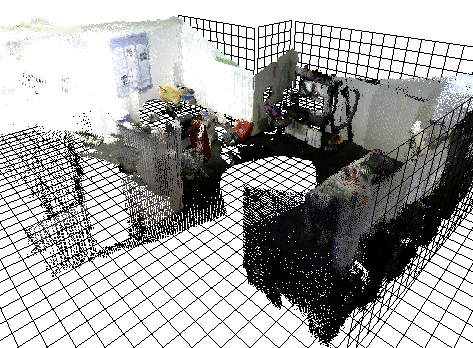
\includegraphics[width=2.0in]{images/ch2/unit21}
                \caption{Apartment}
                \label{fig:RECON_UNIT}
        \end{subfigure}%
        \begin{subfigure}[b]{2.0in}
                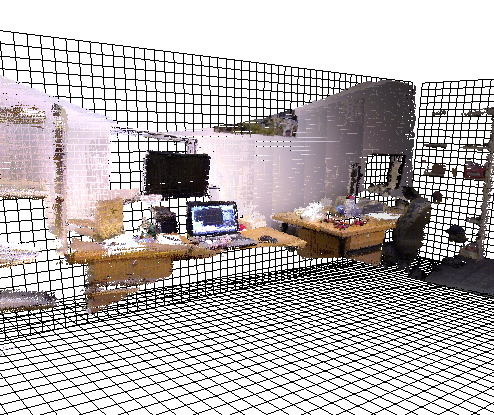
\includegraphics[width=2.0in]{images/ch2/officeA}
                \caption{Office}
                \label{fig:RECON_OFFICE}
        \end{subfigure}%
        \begin{subfigure}[b]{2.0in}
                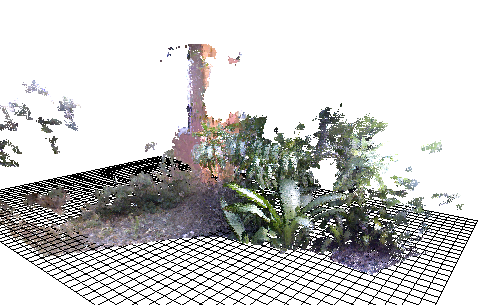
\includegraphics[width=2.0in]{images/ch2/outdoorA}
                \caption{Garden}
                \label{fig:RECON_GARDEN}
        \end{subfigure}
       \caption{Reconstructed Scenes.}
       \label{fig:RECONSTRUCTIONS}
\end{figure*}

Two indoor environments (Apartment and Office) as well as one outdoor environment (Garden) were reconstructed and are shown in figures \ref{fig:RECON_UNIT}, \ref{fig:RECON_OFFICE} and \ref{fig:RECON_GARDEN} respectively. \\

The Apartment reconstruction was recorded by moving through a room and rotating the camera. Some frames contain featureless walls whilst others had contrast shifts due to the camera's automatic contrast feature. Despite these obstacles, accurate reconstruction was achieved. \\

The office reconstruction was also generated by rotating the camera about the y-axis while moving backwards. FVR is a closed form solution yet its accuracy is still comparable to existing feature based SLAM methods. Typical feature based methods work well with indoor environments where local features are readily distinguishable and easy to match. They do not tend to work as well with complex outdoor scenes where feature confusion is likely. To assess performance in such outdoor scenes, a garden scene containing bushes, plants and a ground covering of bark and rocks was used. In the case of a feature matching approach this scene would likely result in feature confusion, making camera tracking difficult. The proposed method was able to produce a good quality reconstruction. Hence, the FVR approach readily overcomes difficulties common to feature matching methods.             


\section{Quantitative Results}



%pose estimation experiments

\subsection{Pose Estimation Results}

These experiments measured registration error for the data sets mentioned in the test data section. As mentioned, different camera movements and scene types are used. Different camera movements such as translation, rotation and zoom were used. The different scenes used include: in-door, out-door, low-textured areas, large object frames areas and areas which include texture confusion. \\


\begin{figure*}[t]
\centering
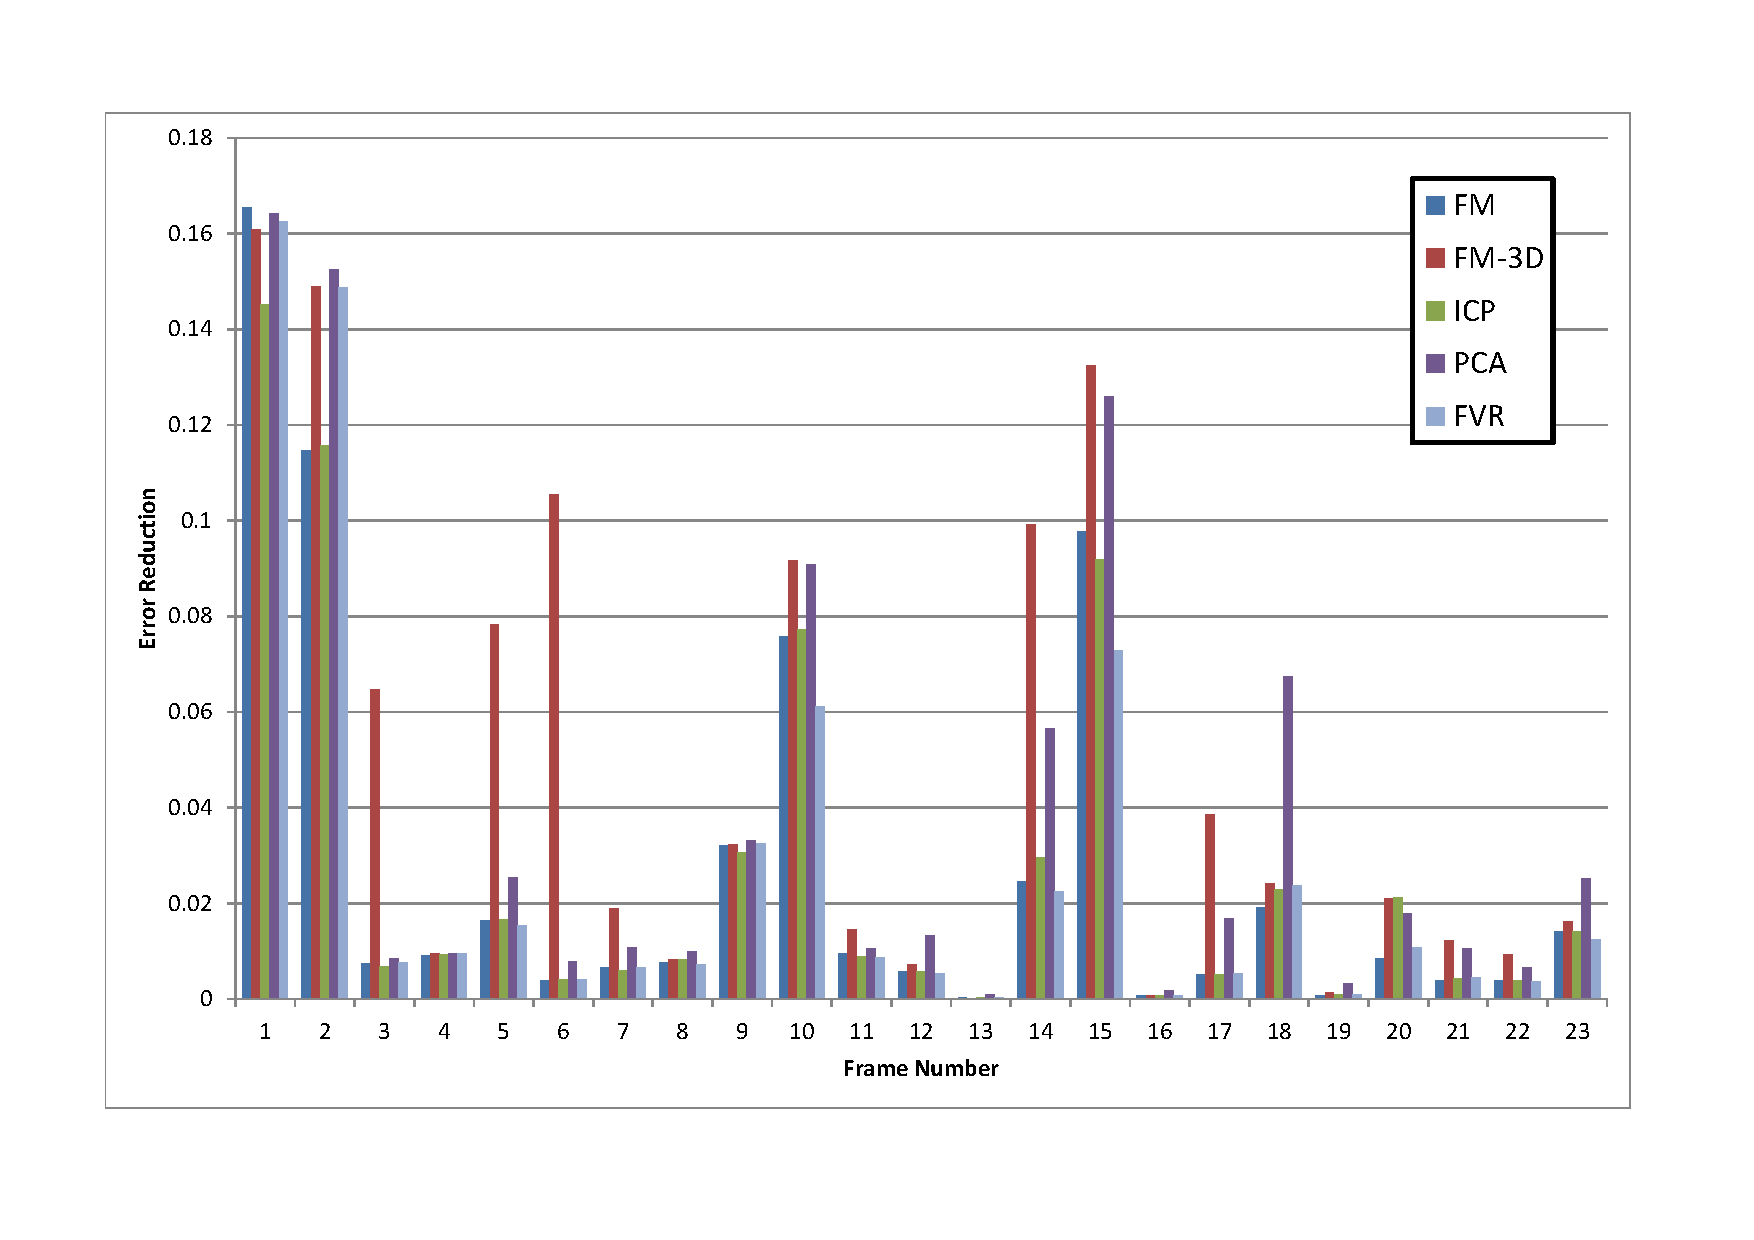
\includegraphics[width=6.0in]{images/results/Apartment_Texture_Rotate}
\caption{Registration Error for the Apartment Y-Axis Rotation Data Set}
\label{fig:PET0}
\end{figure*}

The first experiment was performed with the textured apartment data-set \ref{fig:PET0}. In each of these graphs, the x-axis represents the frame number (in which the previous frame was matched to) and the y-axis represents the registration error in Hausdorff distance relative to performing zero registration. For identical point-clouds, a Hausdorff error above 1 would mean a failure to register in any way, whilst a 0 would mean a complete registration. Since frames do not overlap, it would be improbably to get 0, and a registration error of 1 or above may still be considered good, especially if there was not much overlap in the first place. \\


\begin{figure*}[t]
\centering
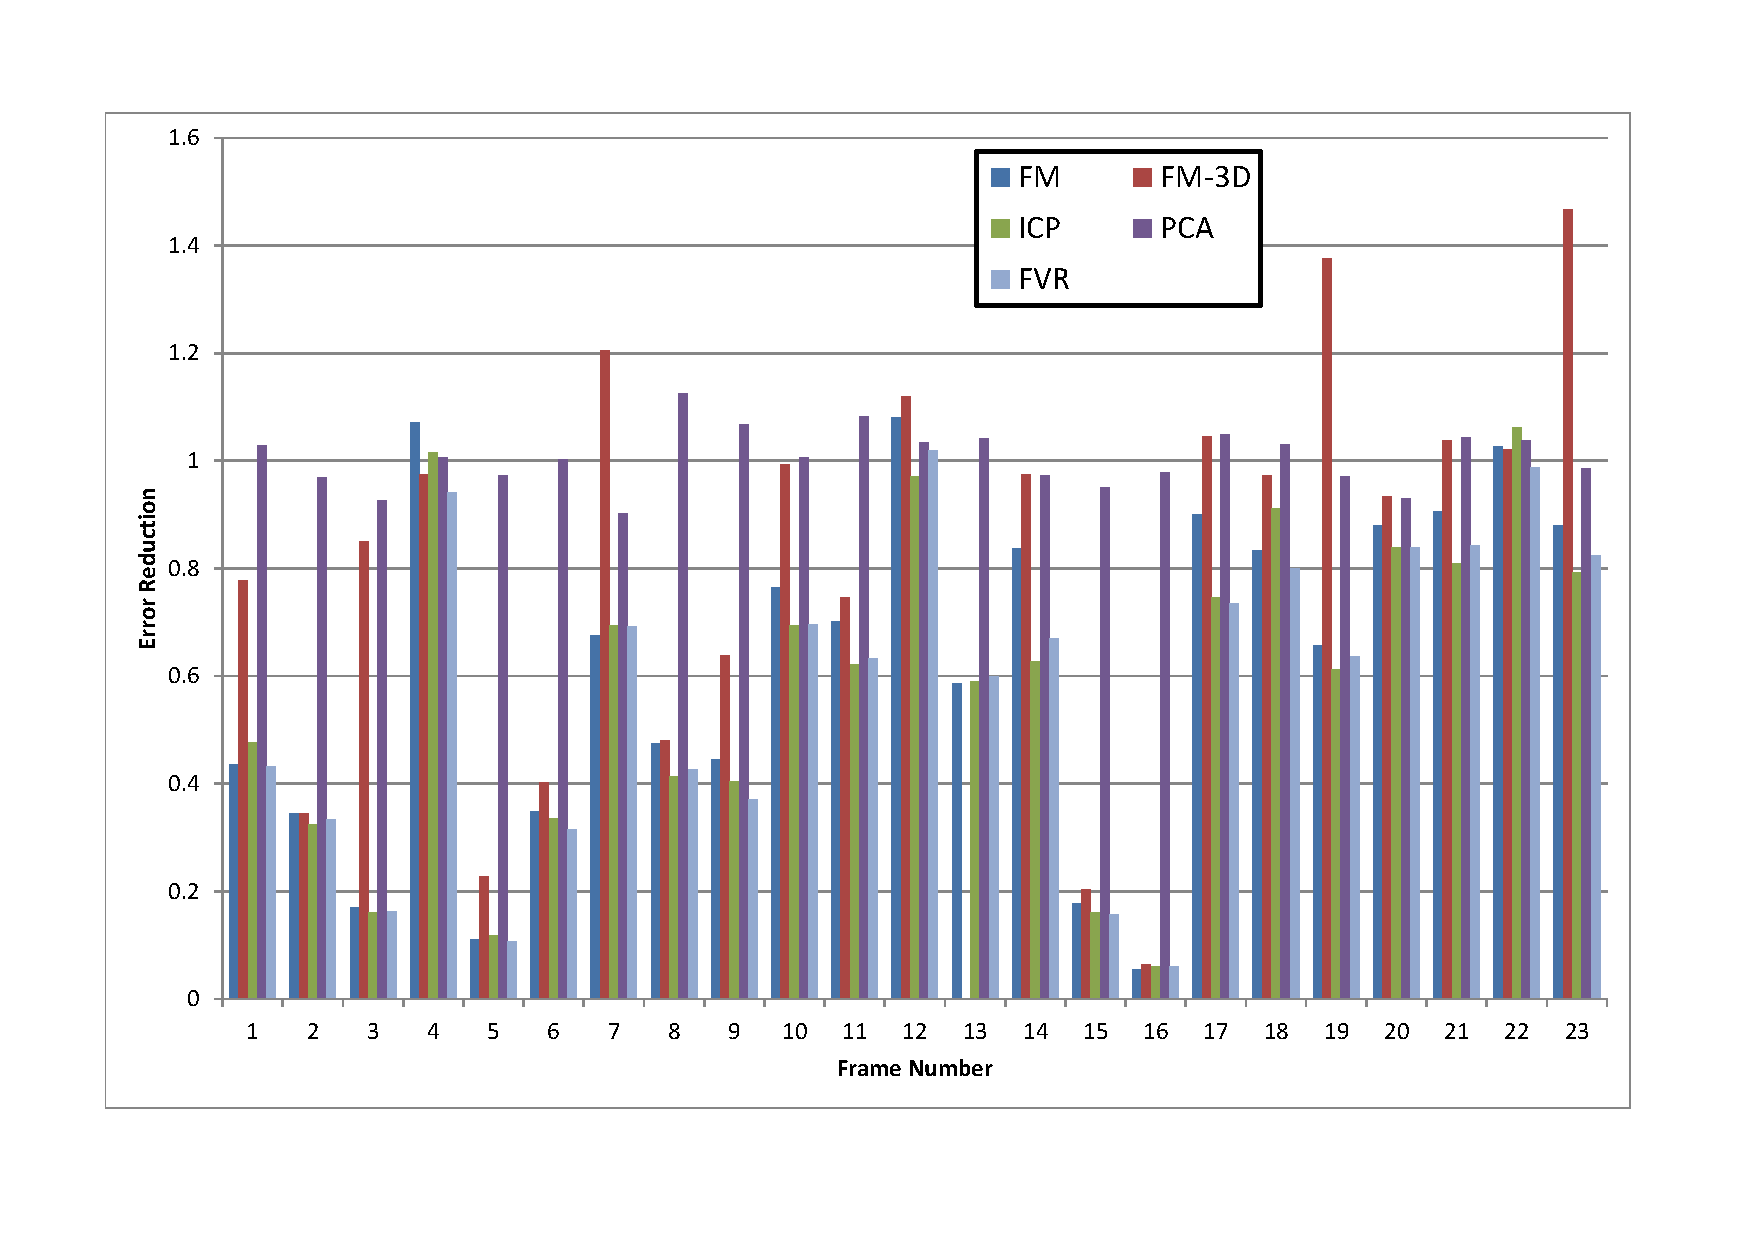
\includegraphics[width=6.0in]{images/results/Apartment_Texture_Rotate_XAxis}
\caption{Registration Error for the Apartment X/Y-Axis Rotation Data Set}
\label{fig:PET1}
\end{figure*}

In figure \ref{fig:PET0}, feature-matching, 3D-feature-matching, ICP, PCA and Fourier Volume Registration (FVR) were tested. In the first frame, FVR only outperformed feature-matching and PCA. In a few of the frames, the 3D feature matching and the PCA methods performed poorly relative to the reset, on other frames they were on par with others. In some frames FVR outperformed the others, this occurred on 13 out of the 23 frames tested (about 60\%). This was not completely expected as for this scene, where much texture is present, feature matching should have dominated. The frames were not highly separated so ICP should have gotten a better result too. Although ICP could be said to be very consistent.

\begin{figure*}[t]
\centering
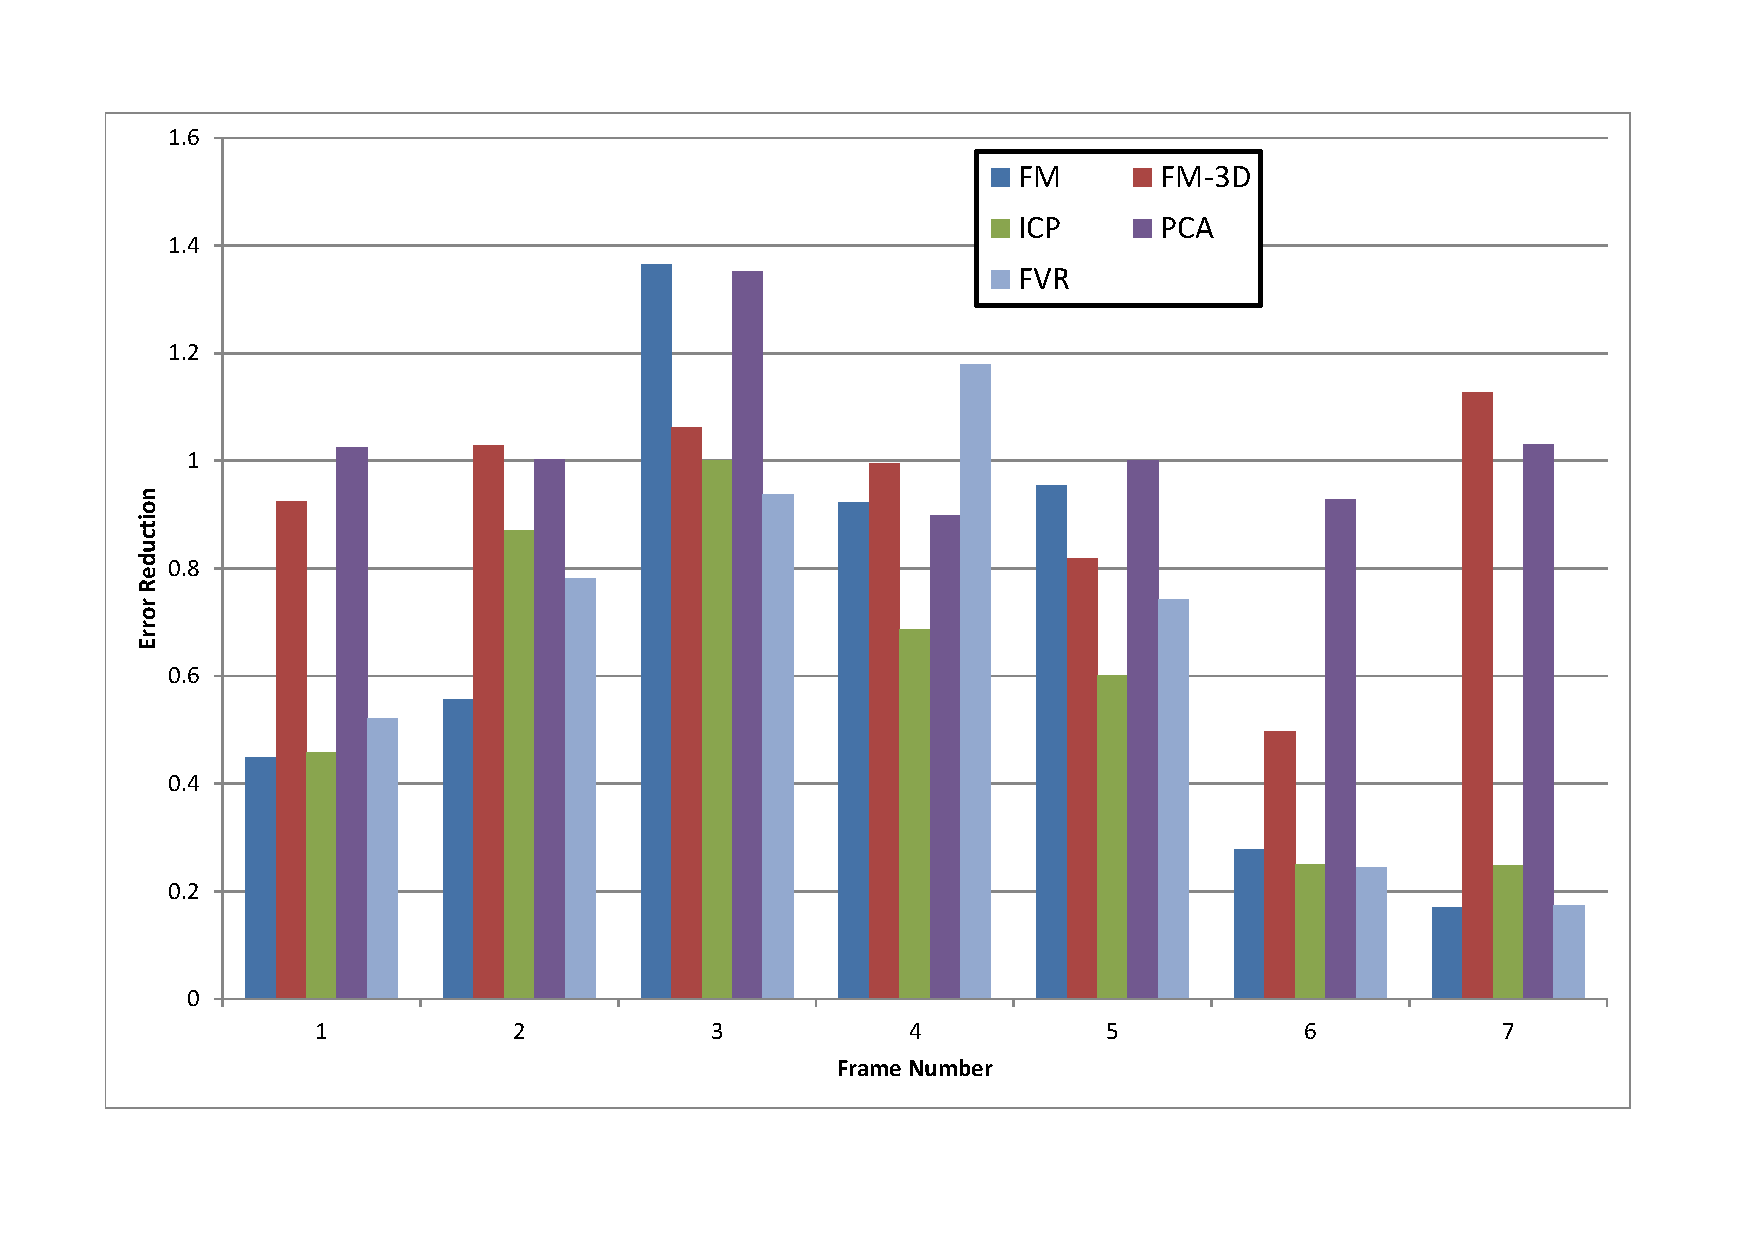
\includegraphics[width=6.0in]{images/results/Boxes_Texture_Rotate}
\caption{Registration Error for the Boxes Y-Axis Rotation Data Set}
\label{fig:PET2}
\end{figure*}

Figure \ref{fig:PET1} shows registration errors for the same scene, the apartment, this time the camera is moved about the x-axis predominantly, again it contains lots of texture. In a about 60\% of the frames, FVR either outperforms or matches the best performing algorithm. Here, ICP and 2D-feature matching are also very competitive, with 3D-feature-matching and PCA failing. In the case of PCA, when there is not enough overlap PCA fails to compute the principal components well. When FVR uses PCA, it only uses the primary axis, and can iteratively refine the alignment in a second stage.

\begin{figure*}[t]
\centering
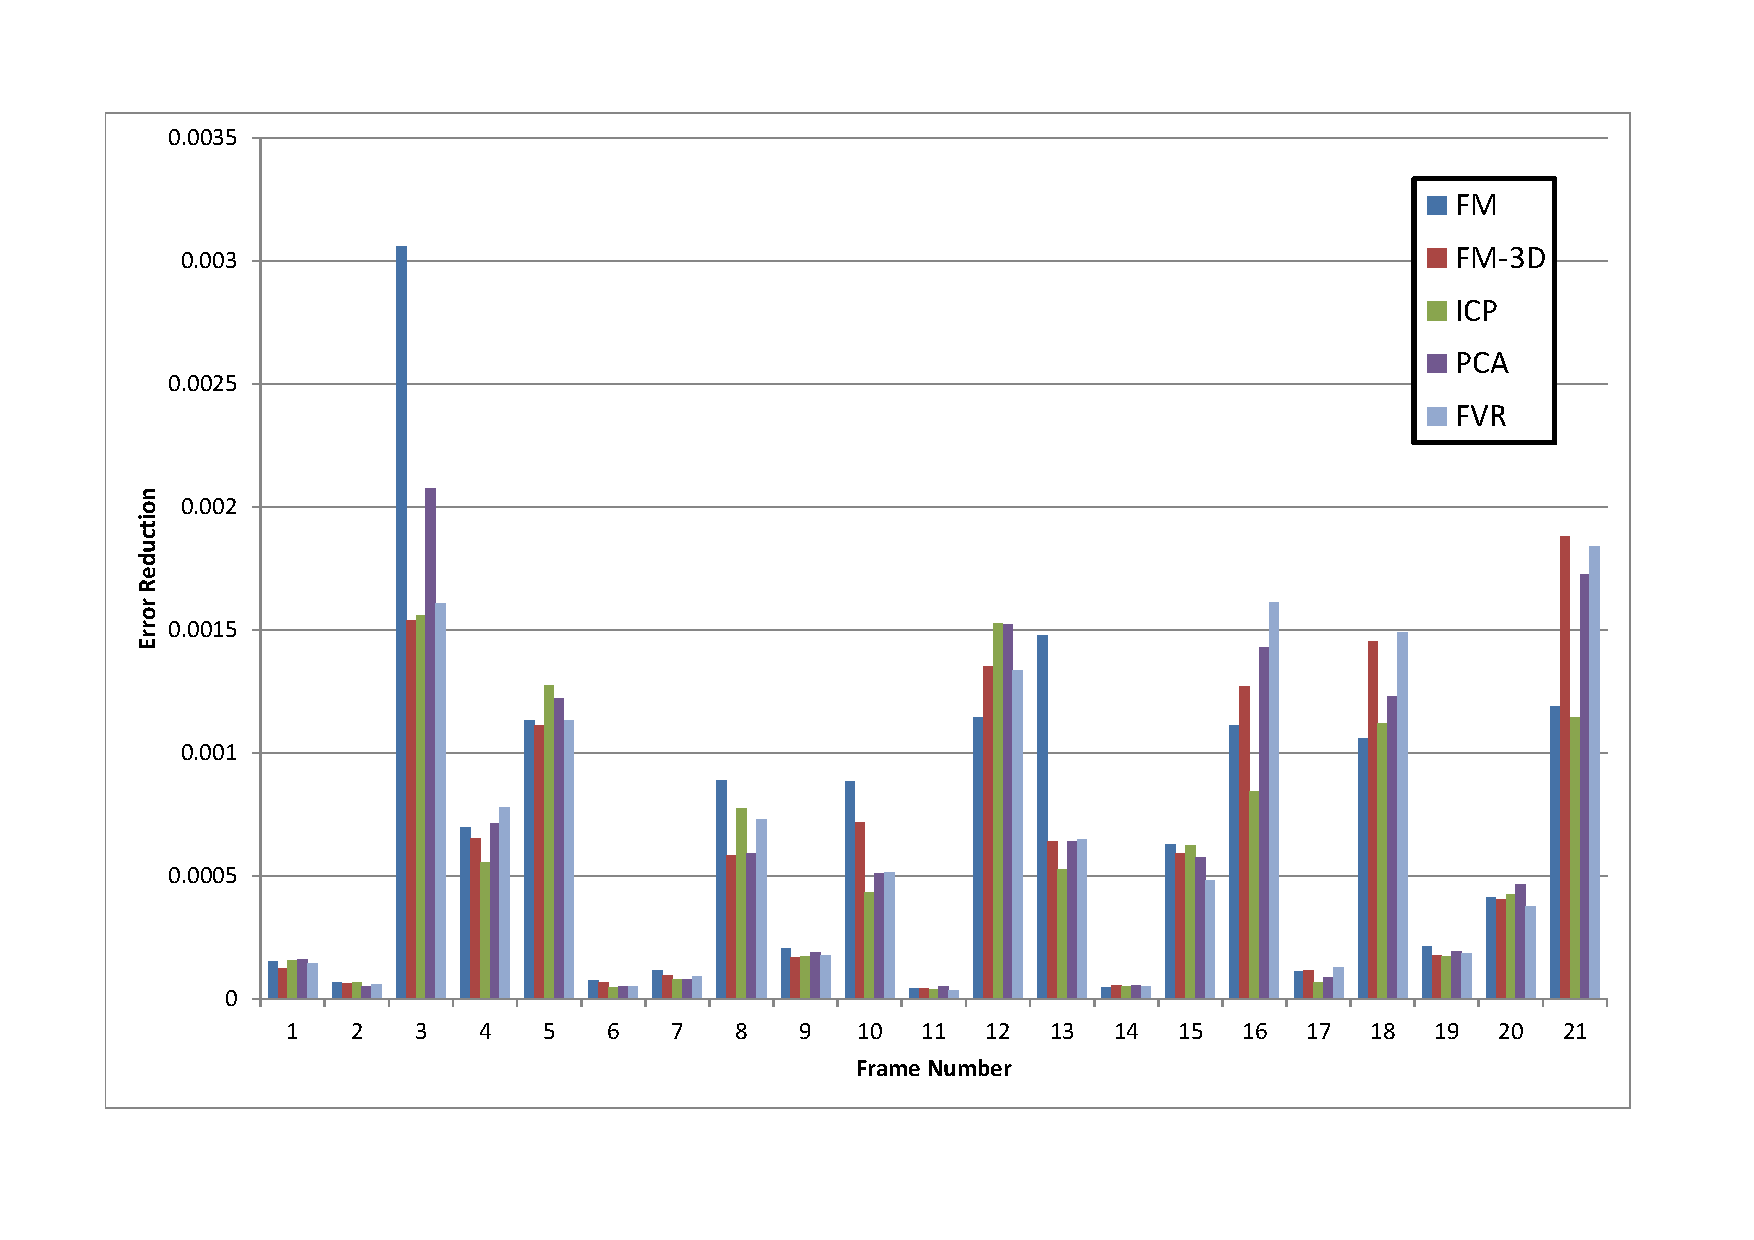
\includegraphics[width=6.0in]{images/results/Boxes_Texture_ZoomOut}
\caption{Registration Error for the Boxes Zoom Data Set}
\label{fig:PET3}
\end{figure*}

In figure \ref{fig:PET2} 7 registration errors are shown in a graph. In 4 out of the 7 frames, FVR outperformed the other algorithms. Note in frame 3, both PCA and feature-matching failed, despite texture being present in the scene. In frames 4 and 5, ICP outperformed the others by a successful margin. 

\begin{figure*}[t]
\centering
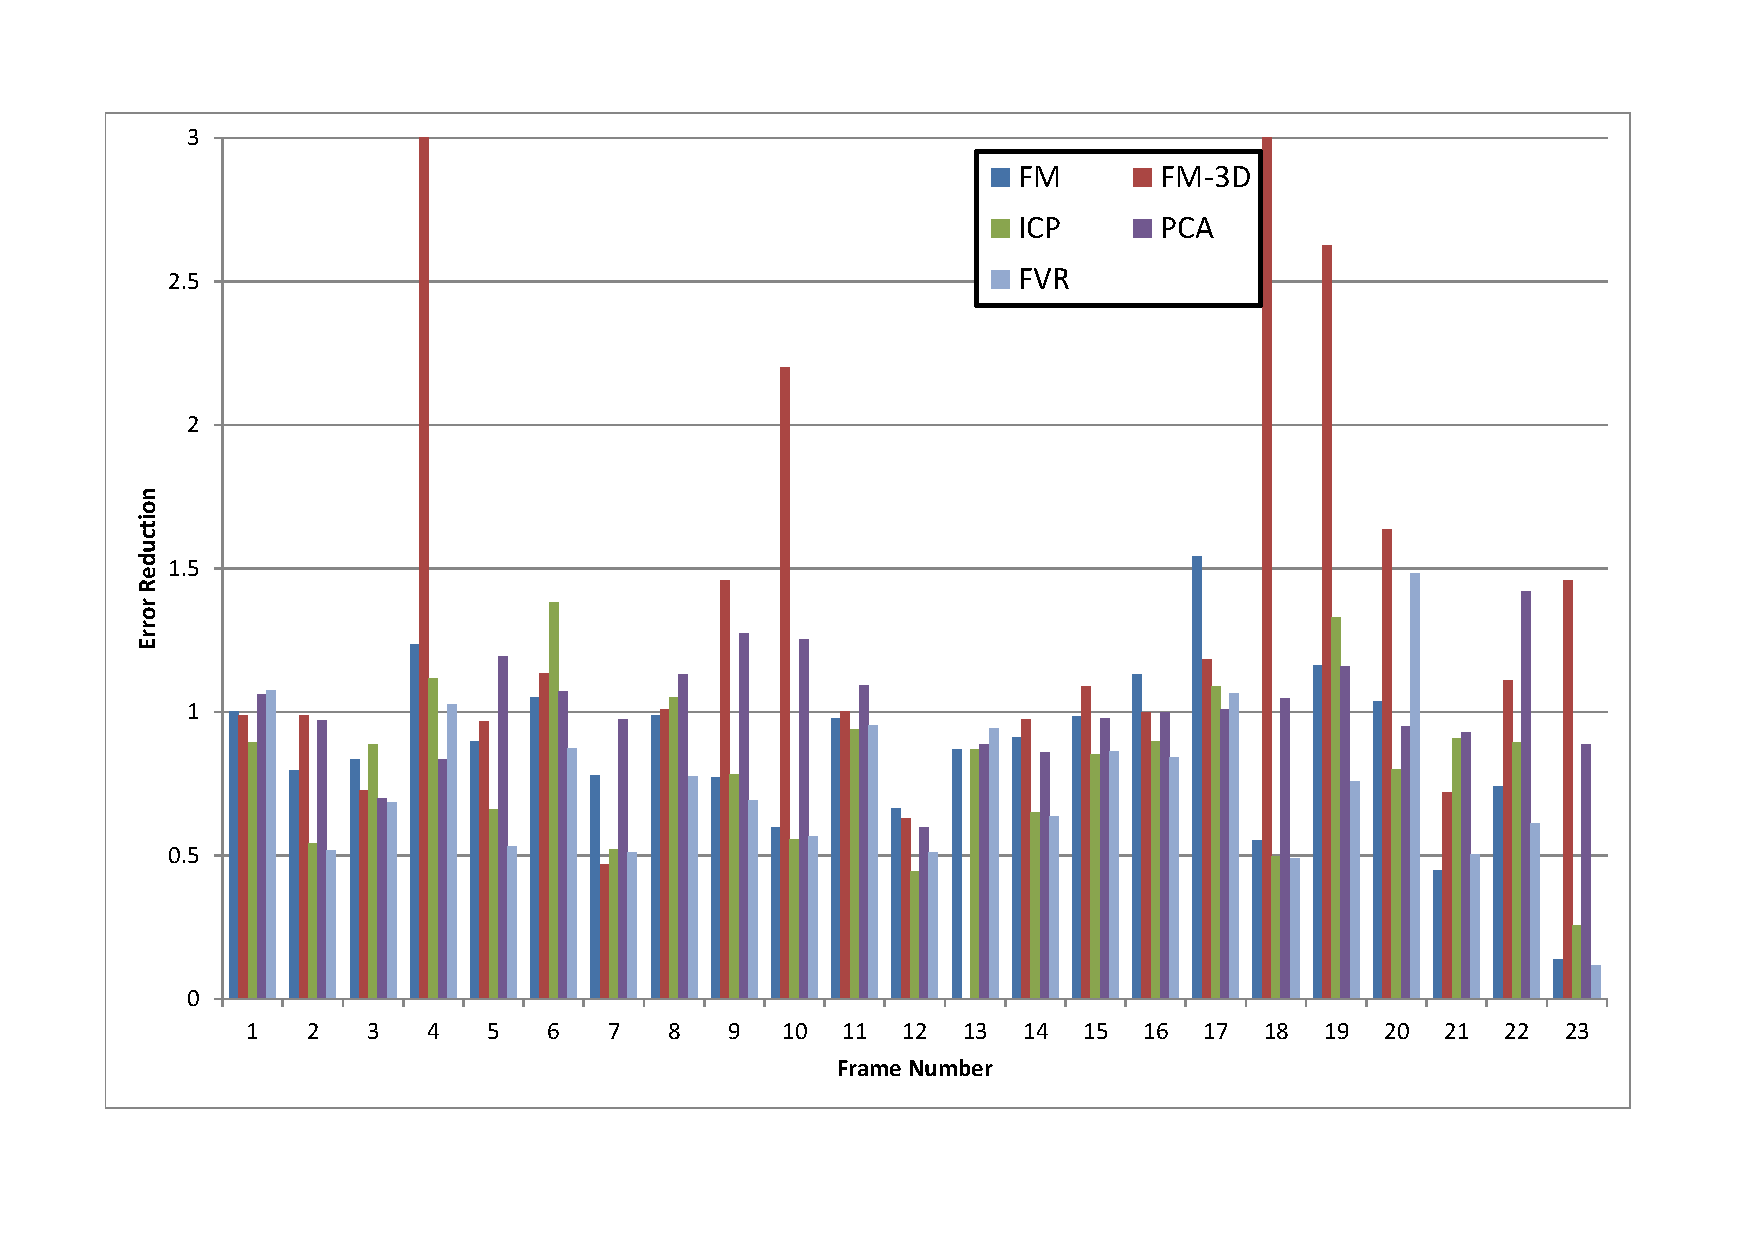
\includegraphics[width=6.0in]{images/results/Desk_Texture_Translation}
\caption{Registration Error for the Desk Translation Data Set}
\label{fig:PET4}
\end{figure*}

Experiment results for the boxes scene where the camera was moved forward, effectively zooming in on the boxes, are shown in figure \ref{fig:PET3}. Here, only 10 out of the 21 (~47\%) of the frames had a registration error lowest or equal for FVR. In a rare case, frame 16 observed a worst performance by FVR. In frame 3, 2D-feature-matching performed the worst, and towards the last few frames PCA and 3D-feature-matching performed worst.

\begin{figure*}[t]
\centering
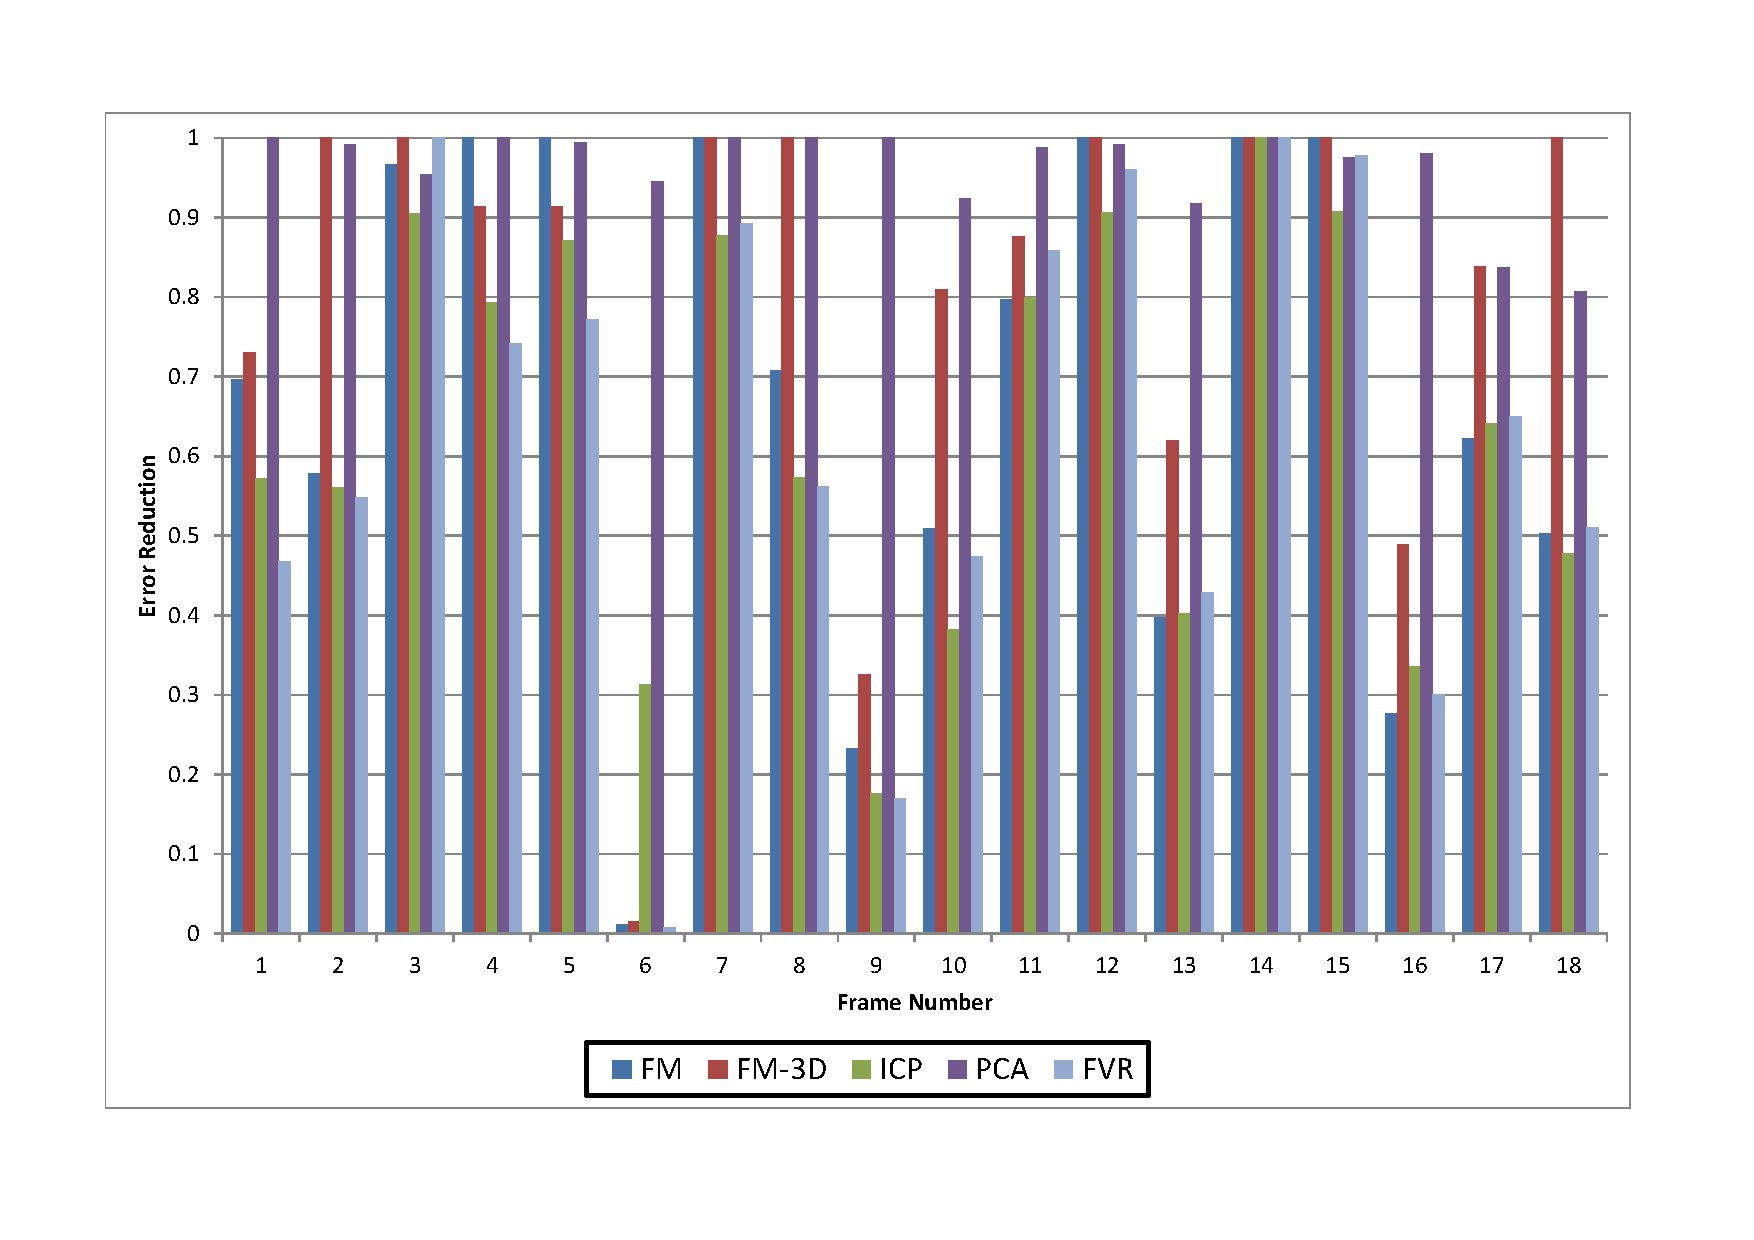
\includegraphics[width=6.0in]{images/results/IndoorSpace_texture_confusion_translation}
\caption{Registration Error for the Texture Confusion Indoor-Space Translation Data Set}
\label{fig:PET5}
\end{figure*}

In ~52\% of the frames of the desk translation data-set in figure \ref{fig:PET4}, the FVR method outperformed others relative to just ~26\% for ICP, ~9\% for 2D-feature-matching and PCA and ~4\% for 3D-feature-matching. This data-set tested for the pose-estimation procedure's ability to align a moving camera along a path. 3D feature matching was a notable poor performer here, ICP and FVR seemed to be strongest. 


\begin{figure*}[t]
\centering
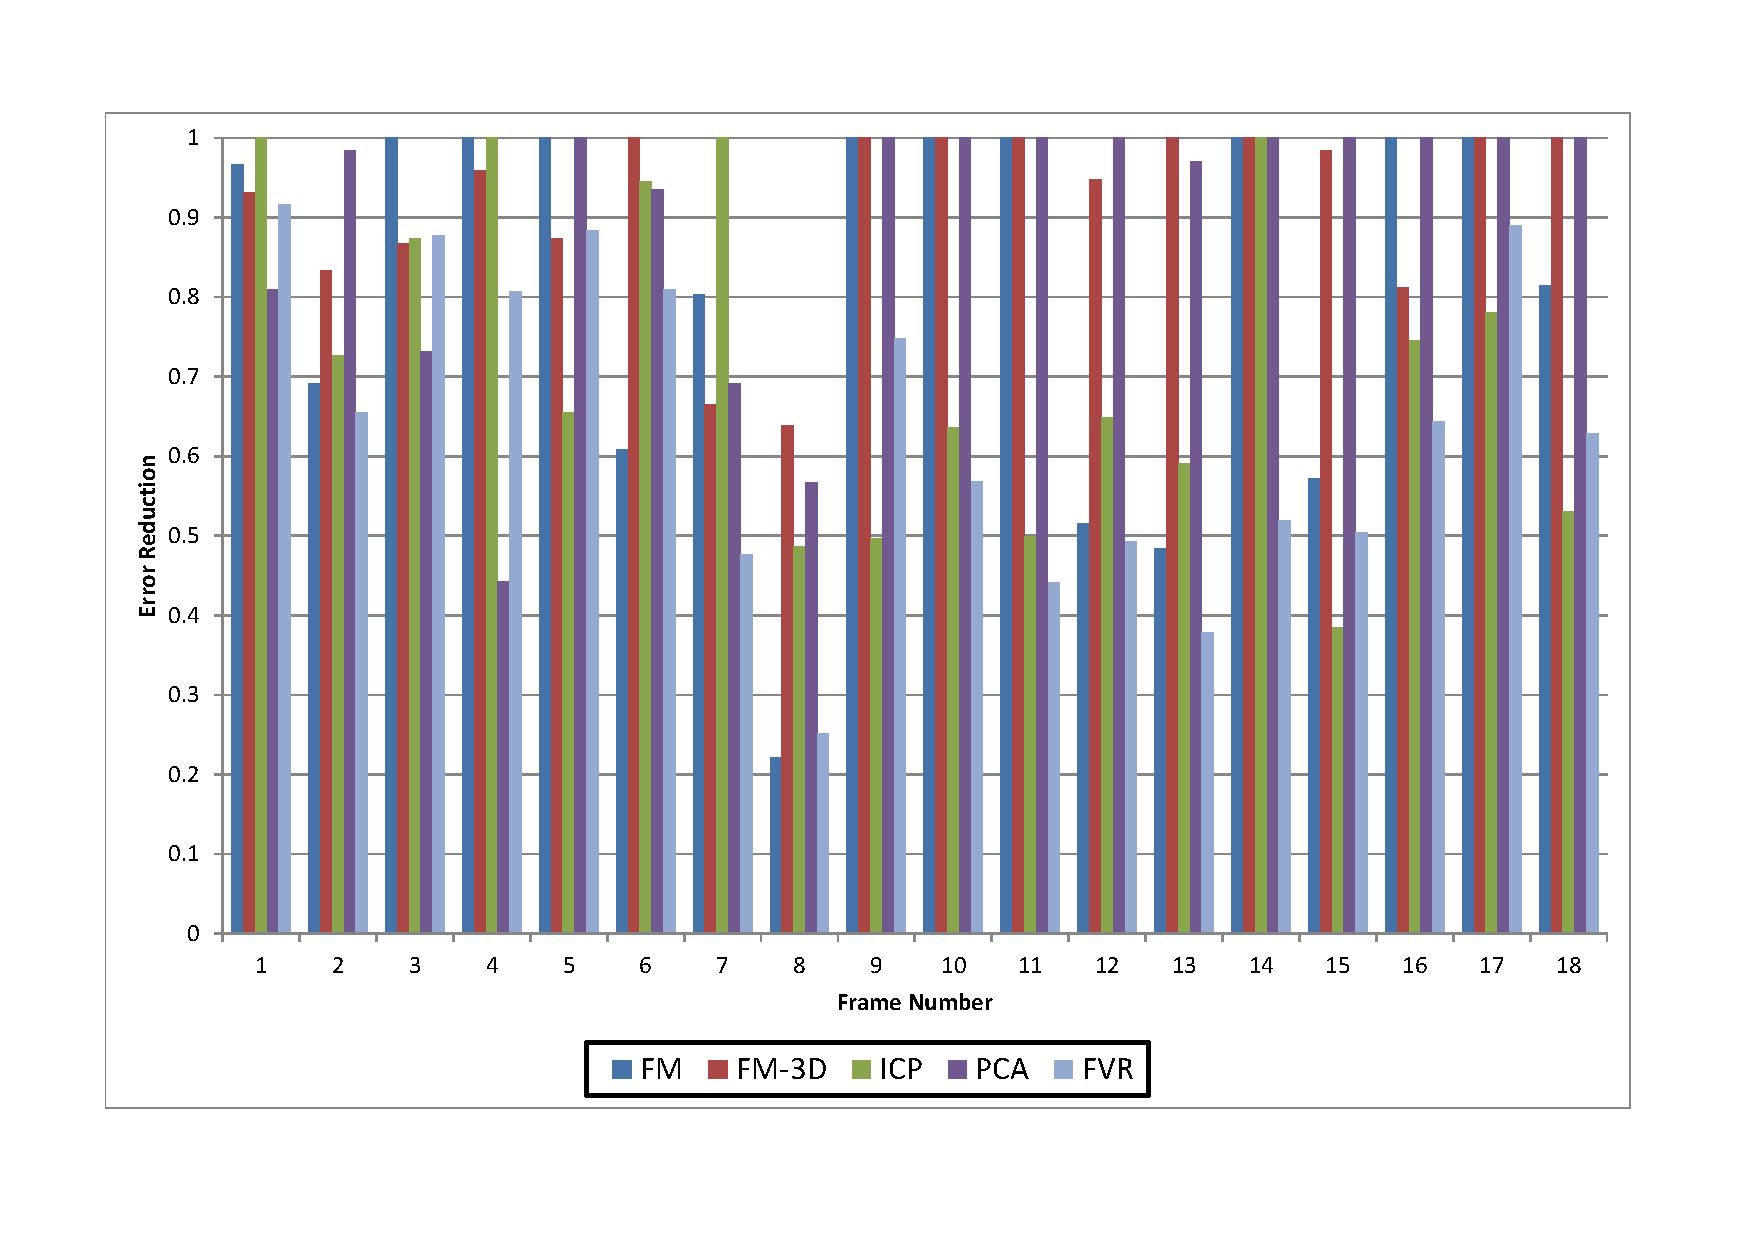
\includegraphics[width=6.0in]{images/results/Kitchen_LittleTexture_Pan}
\caption{Registration Error for the Low-Texture Kitchen Translation Data Set}
\label{fig:PET6}
\end{figure*}

An important data-set tested is the Indoor-Space with texture confusion (figure \ref{fig:PET5}). Here, a small scene was observed, where texture-confusion was present, this makes registration more difficult for all algorithms most notably the feature matching methods. We suspected that ICP, PCA, and FVR would perform best here. Here, around 39\% of the time, FVR performed best. Compared to the best feature-matching method (2D) with ~22\% of performances being the best. Interestingly PCA performed much worse compared with 2D-feature-matching. ICP outperformed others around 33\% of the time, similar to FVR's position but not quite as good. 

Results for the low-textured Kitchen data-set were collected and shown in figure \ref{fig:PET6}. Again around 44\% of the frames had best results given by FVR. Compared with the next best algorithm ICP at ~27\%. In this case, this is expected as the feature-matching methods should perform worse in a low-textured scene. PCA was next best having the best registration ~22\% of the time.

\begin{figure*}[t]
\centering
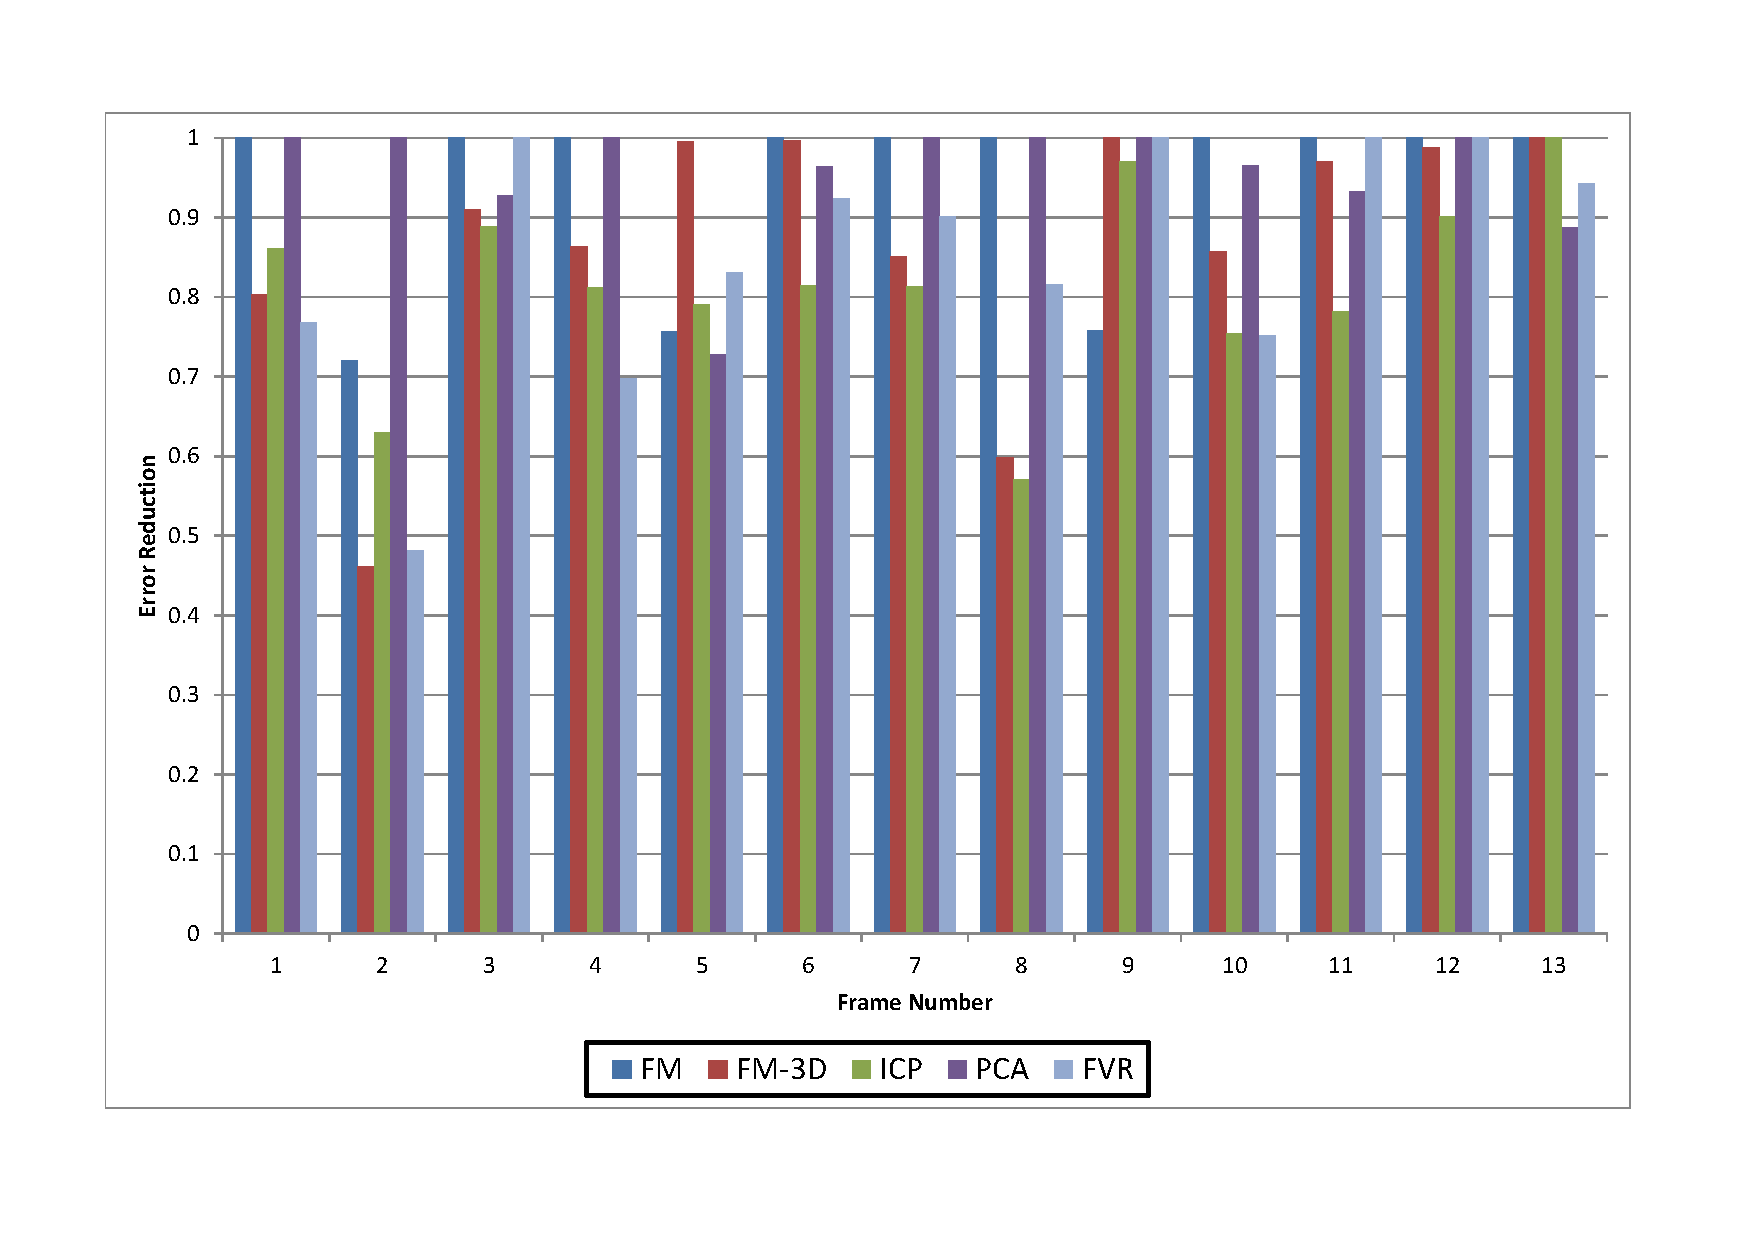
\includegraphics[width=6.0in]{images/results/Kitchen_Little_Texture_Zoom}
\caption{Registration Error for the Low-Texture Kitchen Zoom Data Set}
\label{fig:PET7}
\end{figure*}

Another test for the low-textured Kitchen scene was also performed, this time by moving the camera forward and backwards, zooming in on the scene. In this test, FVR only outperformed the other methods in 3 out of the 13 frames. ICP outperformed FVR on this data-set, as 6 out of the 5 frames had best results given by ICP. It could also be said that ICP was a little more consistent. Interestingly 3D-feature-matching outperformed the 2D counterpart.

\begin{figure*}[t]
\centering
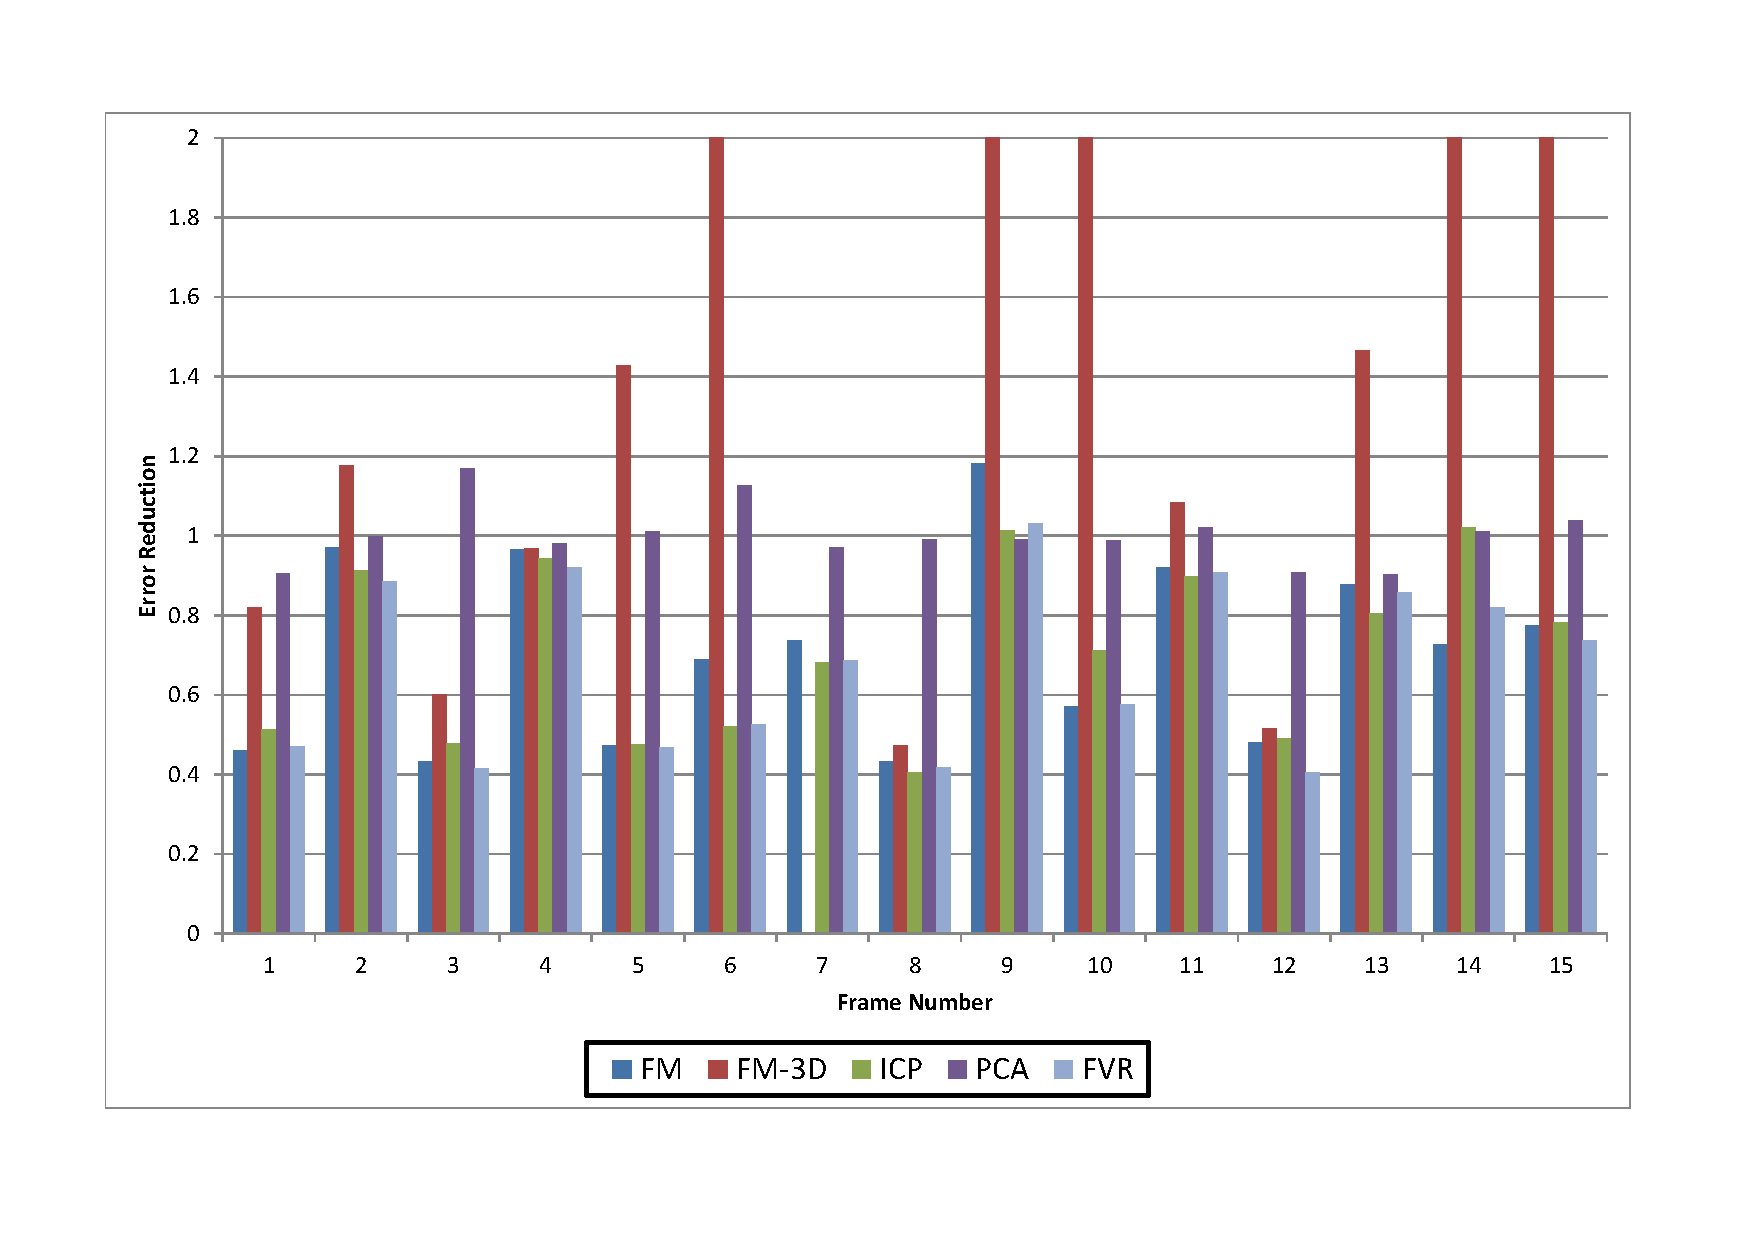
\includegraphics[width=6.0in]{images/results/Office_TexturedItems_Translation}
\caption{Registration Error for the Office Translation Data Set}
\label{fig:PET8}
\end{figure*}

In the results for the Textured Office set (figure \ref{fig:PET8}), FVR matched or beat the other algorithms 80\% of the time. 2D-feature matching also performed well but did not manage to best FVR most of the time. This results shows that, to our surprise, FVR not only works well compared to other algorithms in scenes with little or no texture or in scenes where feature confusion is high, but also in high texture scenes where feature-matching should have an advantage.


\begin{figure*}[t]
\centering
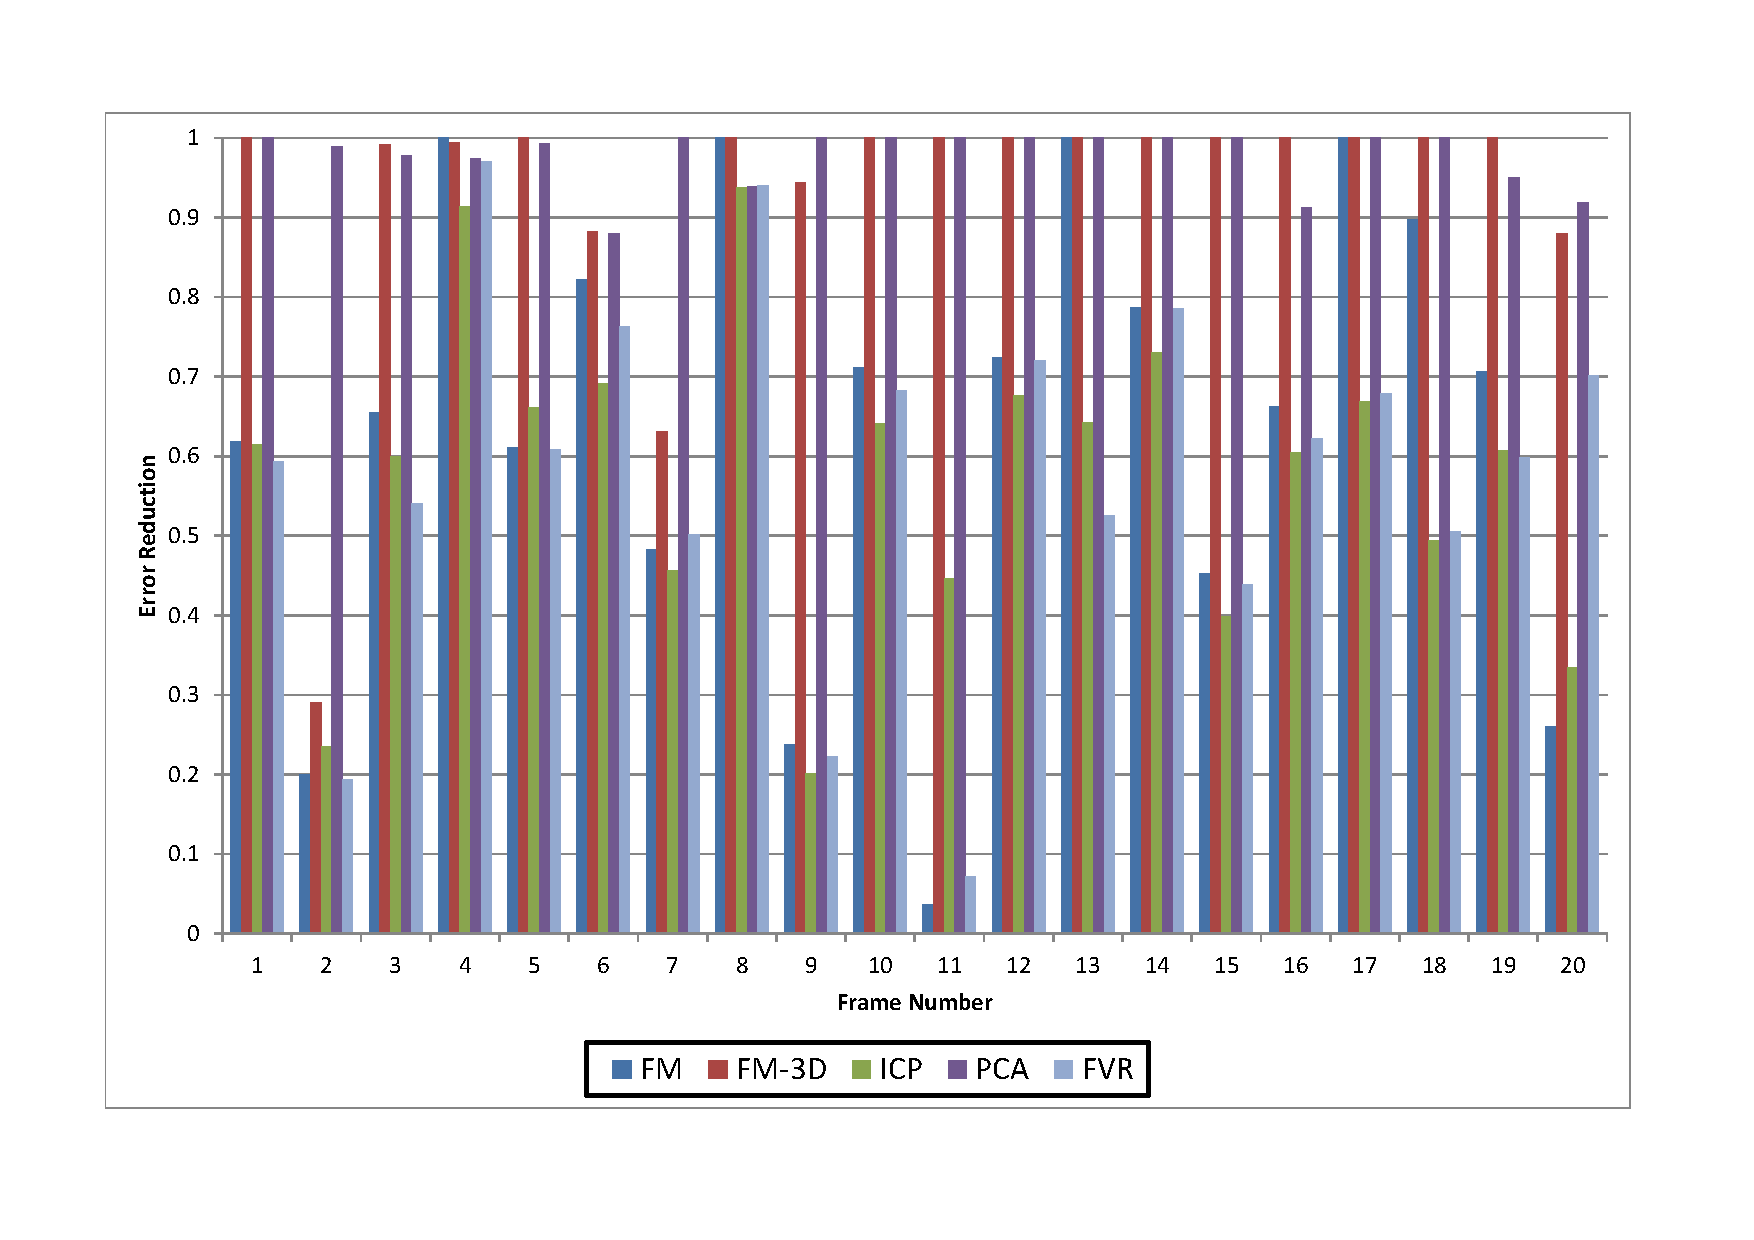
\includegraphics[width=6.0in]{images/results/Office_Texture_blind_spot_rotation}
\caption{Registration Error for the Office Centered Object Rotation Data Set}
\label{fig:PET9}
\end{figure*}

Figure \ref{fig:PET9} shows results for the centred object rotation scene. Here, a large divider was placed in the middle of two desks. The idea was to create an environment where the large divider could throw off the effects of PCA and FVR and give an advantage to the feature matching approaches and ICP. Interestingly, around 35\% of the time, FVR had the best result. 2D-feature-matching outperformed the 3D counterpart but only got the best result 10\% of the time. ICP on the other hand got the best result for around 55\% of the frames. It is suspected that ICP is able to use the large divider as an anchor which would make it more robust to non-overlapped data.

\begin{figure*}[t]
\centering
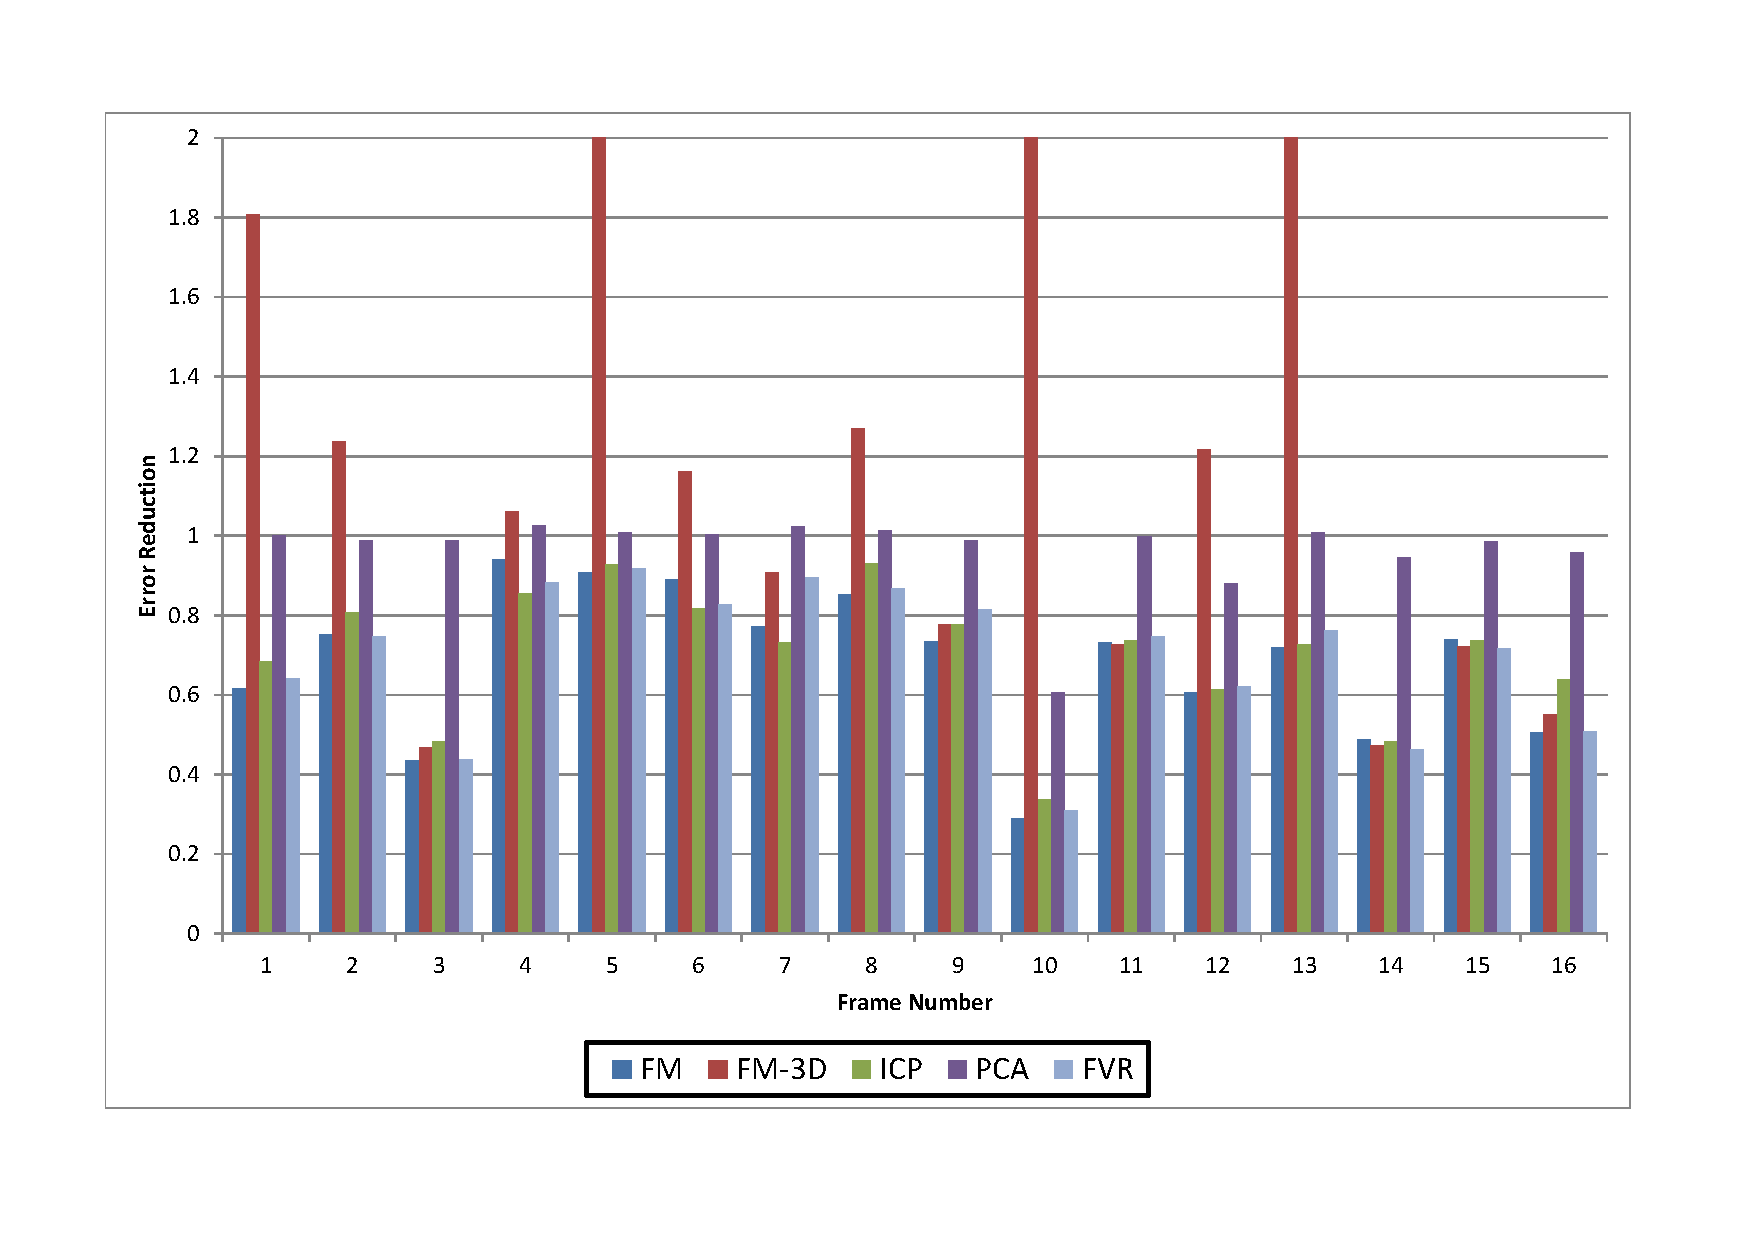
\includegraphics[width=6.0in]{images/results/Office_Texture_Rotate_XAxis}
\caption{Registration Error for the Office X/Y-Axis Rotation Data Set}
\label{fig:PET10}
\end{figure*}

Another experiment where the scene was filmed with the camera rotated predominantly about the x-axis is shown in figure \ref{fig:PET10}, this time 2D-feature-matching, ICP and FVR all performed similarly, with only PCA and 3D-feature-matching failing to get good registrations. 

\begin{figure*}[t]
\centering
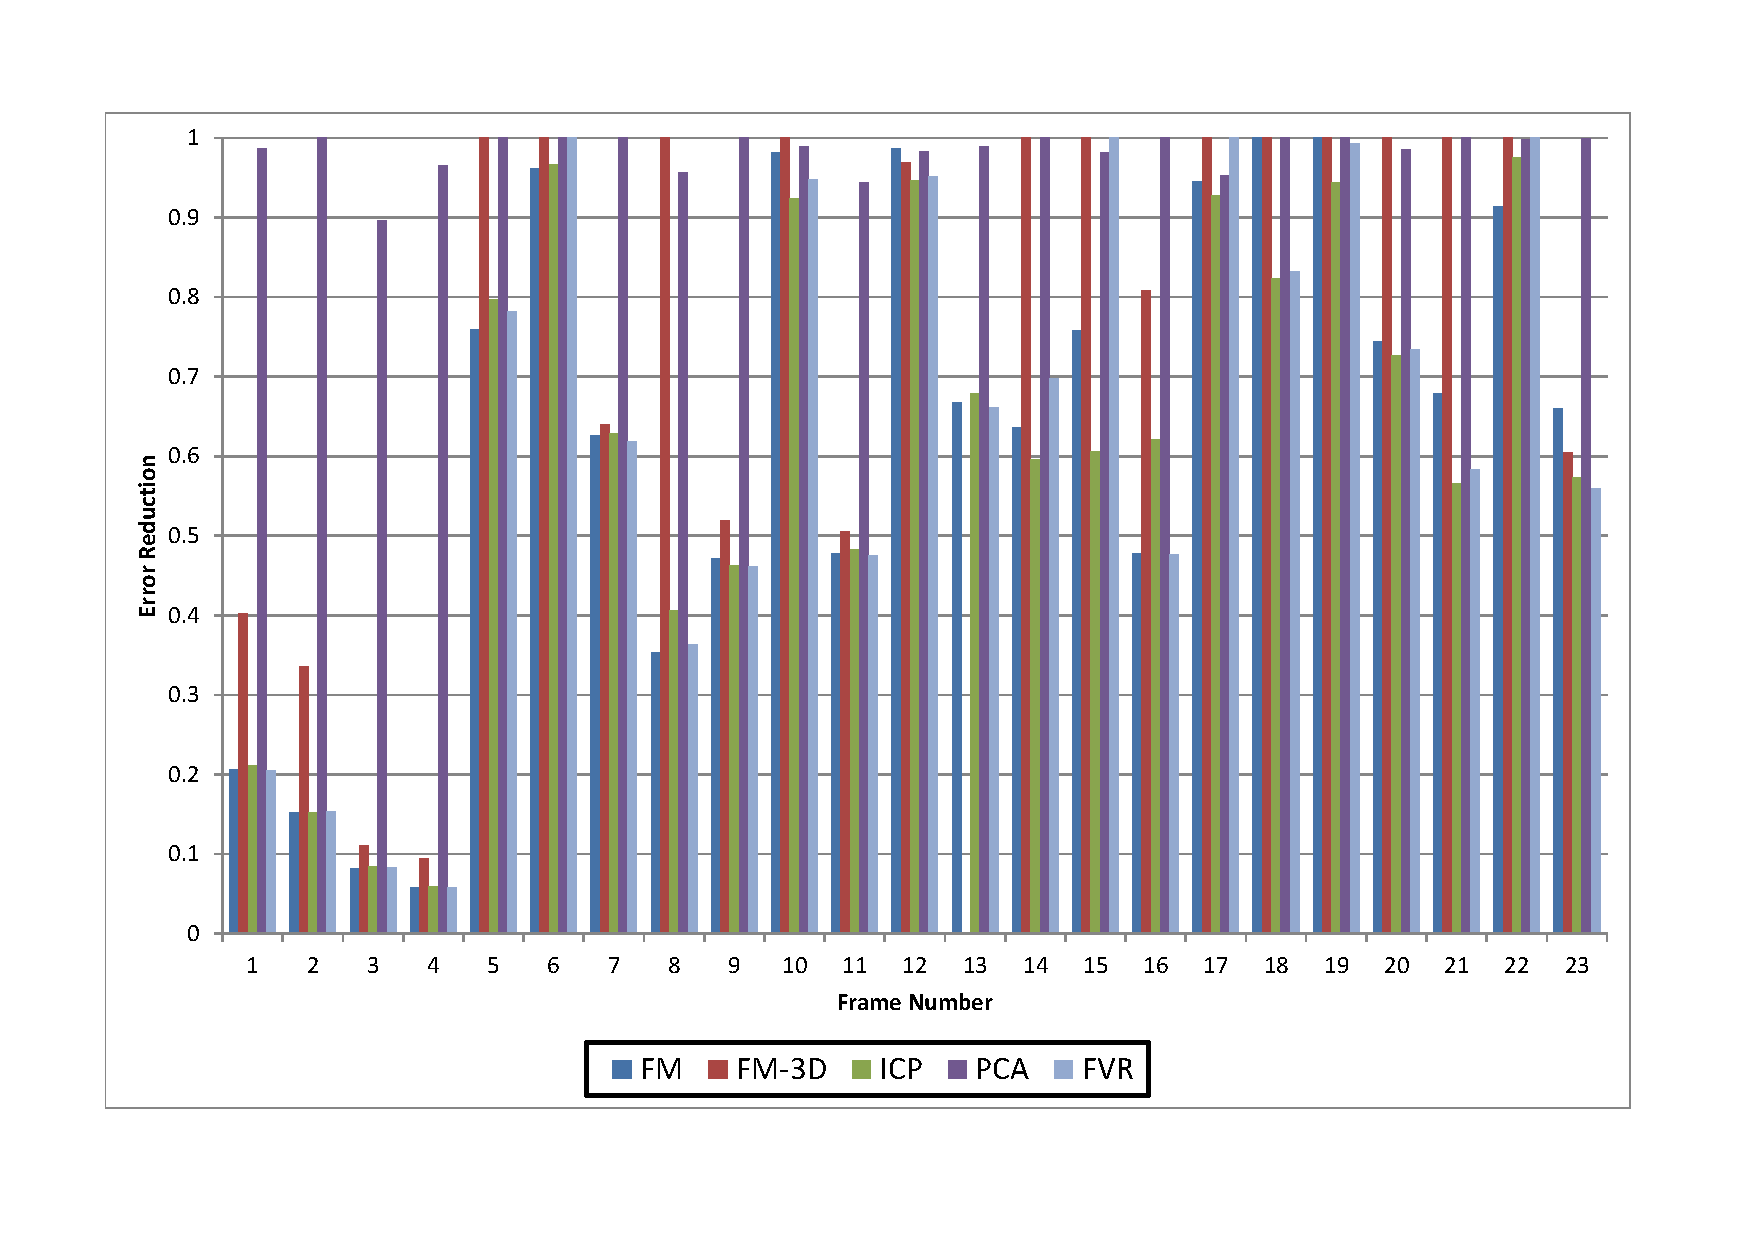
\includegraphics[width=6.0in]{images/results/Office_Texture_Rotation}
\caption{Registration Error for the Office Y-Axis Rotation Data Set}
\label{fig:PET11}
\end{figure*}

Figure \ref{fig:PET11} shows the registration errors for the Office data-set with camera rotation about the Y-axis. Here, in around 50\% of the cases, FVR outperformed or matched the best result. 2D-feature-matching was next best matching or outperforming the best result around 34\% of the time. Interestingly, PCA performed the worst with this data-set. Because rotation can incur a smaller overlap and thus a large shift in the axes and mean of the principal components, this could be expected.

\begin{figure*}[t]
\centering
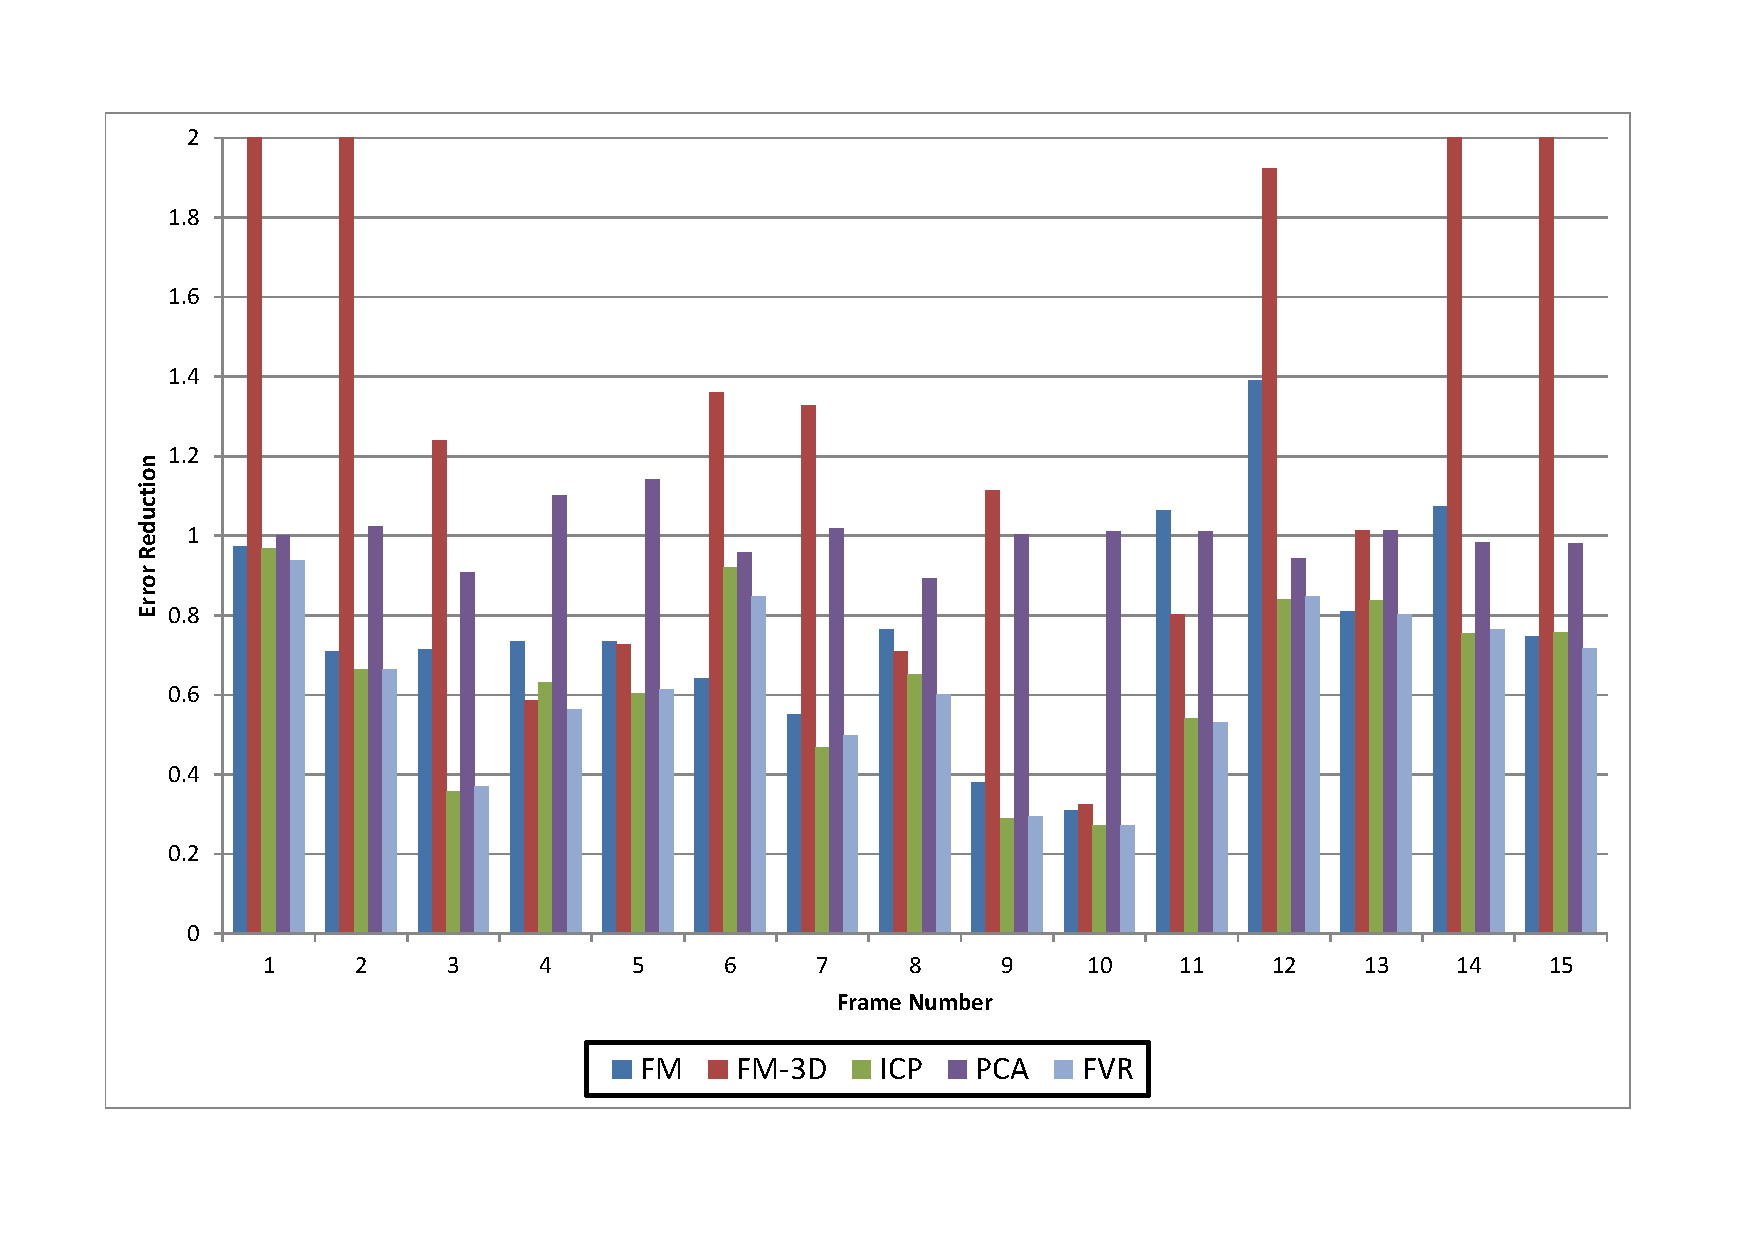
\includegraphics[width=6.0in]{images/results/Office_Texture_Translation}
\caption{Registration Error for the Office Translation Data Set}
\label{fig:PET12}
\end{figure*}

In the Office translation scene, FVR outperformed or matched the other algorithms around 85\% of the time. This shows that the FVR has high accuracy when dealing with translation detection and the registration of 3D data with only translational changes. Here, PCA and 3D-feature matching performed the worst with ICP and 2D-feature matching also being quite consistent and robust.

\begin{figure*}[t]
\centering
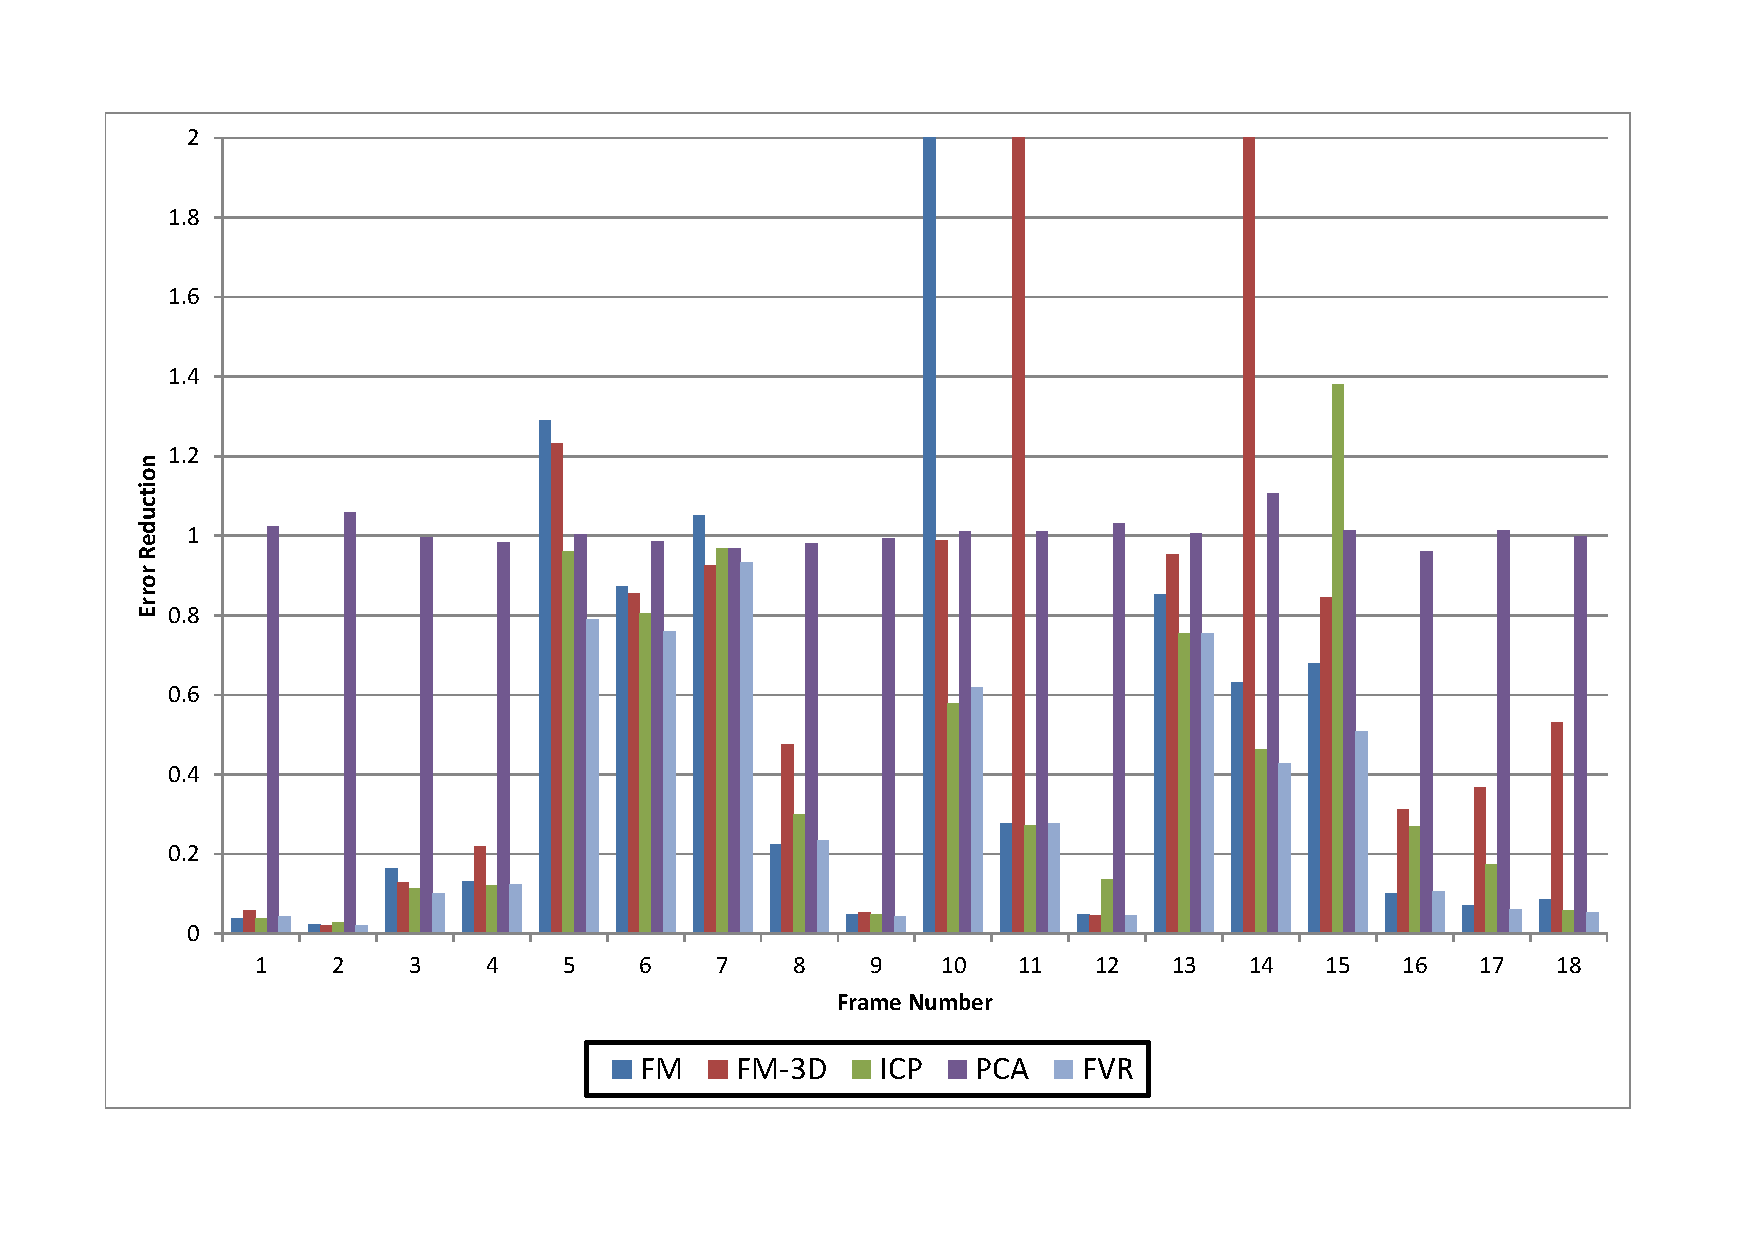
\includegraphics[width=6.0in]{images/results/Outside_No_Texture_Rotation}
\caption{Registration Error for the Little Texture Outdoors Rotation Data Set}
\label{fig:PET13}
\end{figure*}

Figure \ref{fig:PET13} shows results for an outdoors scene with little texture, here the camera was rotated about an origin. In this case, PCA performed the worst, and 3D-feature-matching also failed several times. The only algorithm which did not fail once was FVR. In this test, FVR outperformed or matched the other algorithms 88\% of the time. This can be explained by FVR's robustness to out-door scenes and scenes with little texture. 

\begin{figure*}[t]
\centering
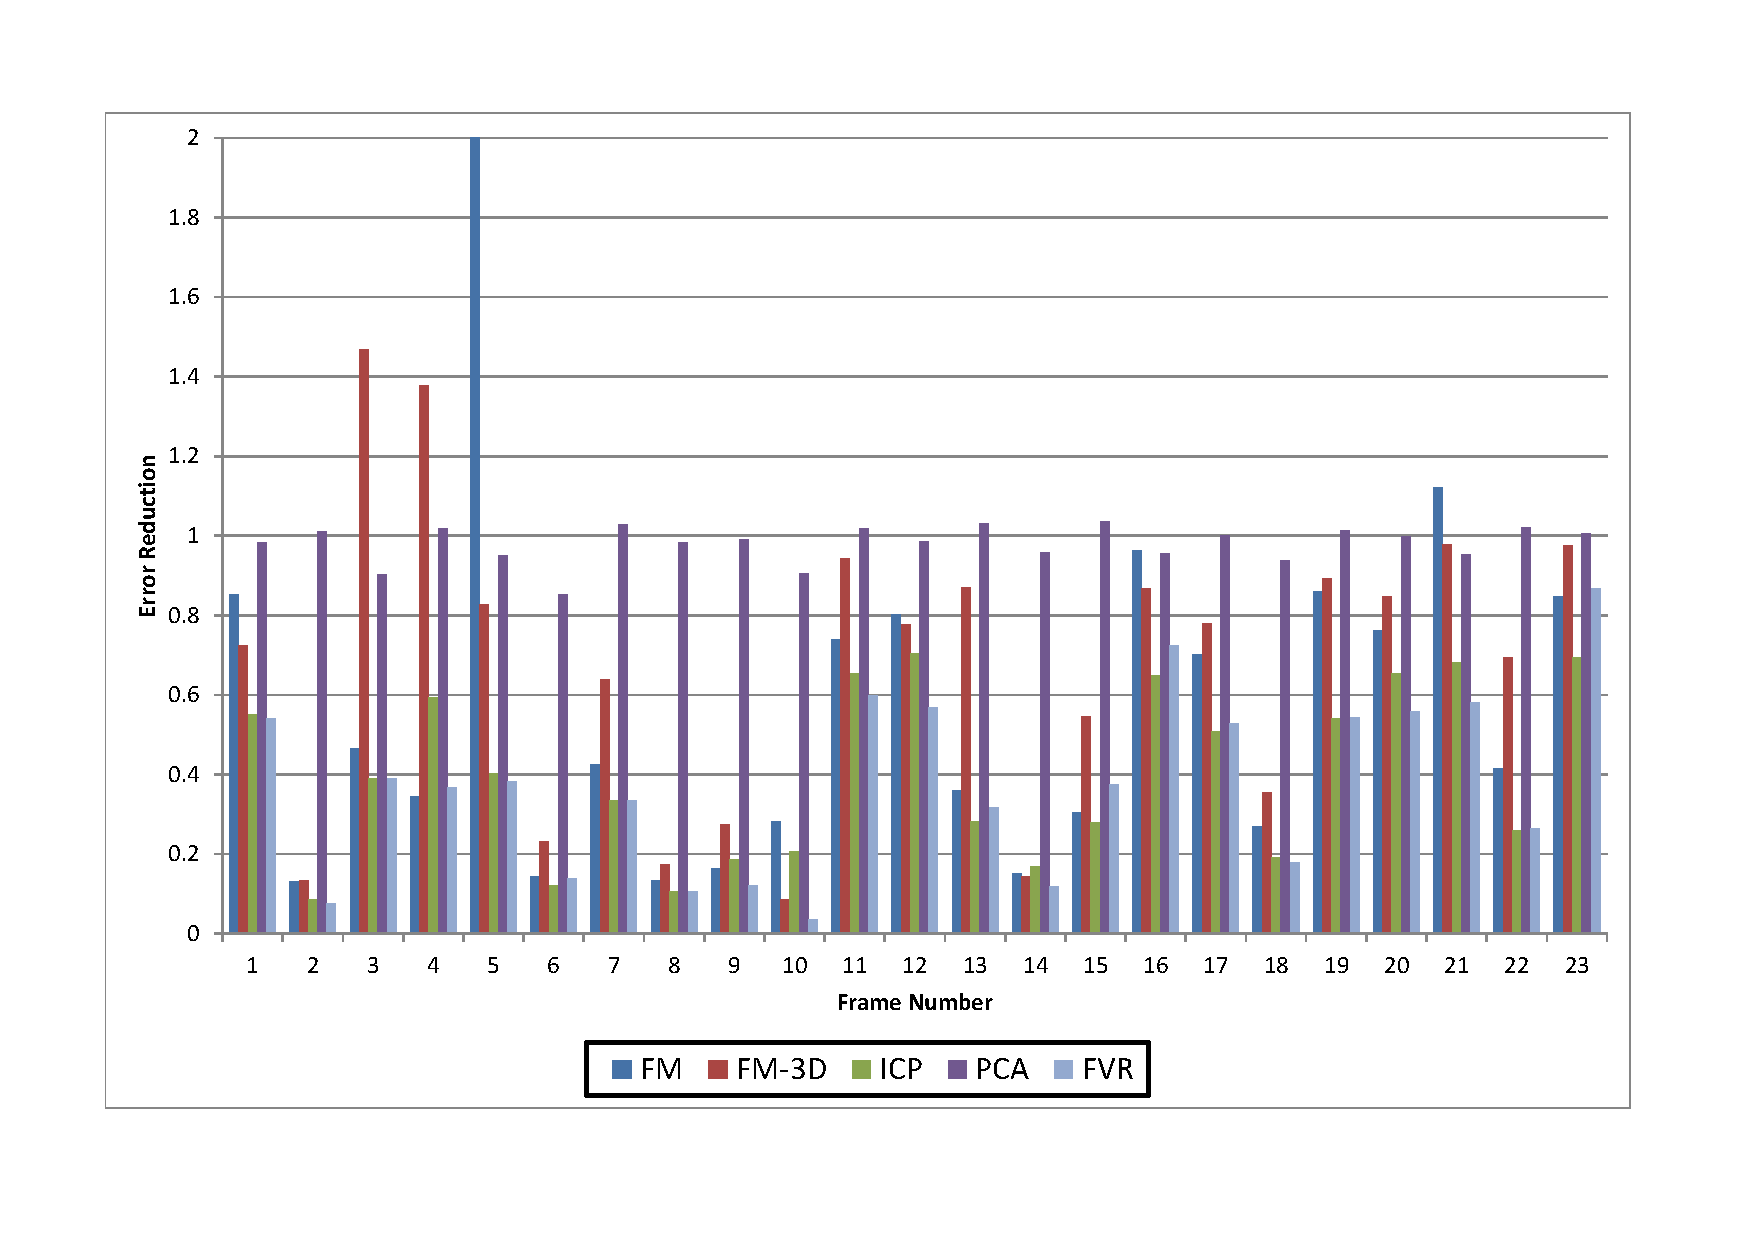
\includegraphics[width=6.0in]{images/results/Outside_No_Texture_Translation}
\caption{Registration Error for the Little Texture Outdoors Translation Data Set}
\label{fig:PET14}
\end{figure*}

Another test using a low-textured out-doors scene was tested where the camera was translated along a path. Results are shown in figure \ref{fig:PET14}. Here again the FVR method dominated recording either the best result or matching best result for around 73\% of the frames. Notably, PCA performed poorly, and both the feature-matching methods failed to register a few times. ICP was more consistent, recoding the best or equivalent result around 47\% of the time. Again, this shows the strength of the FVR method in out-door and low-texture environments. 

\begin{figure*}[t]
\centering
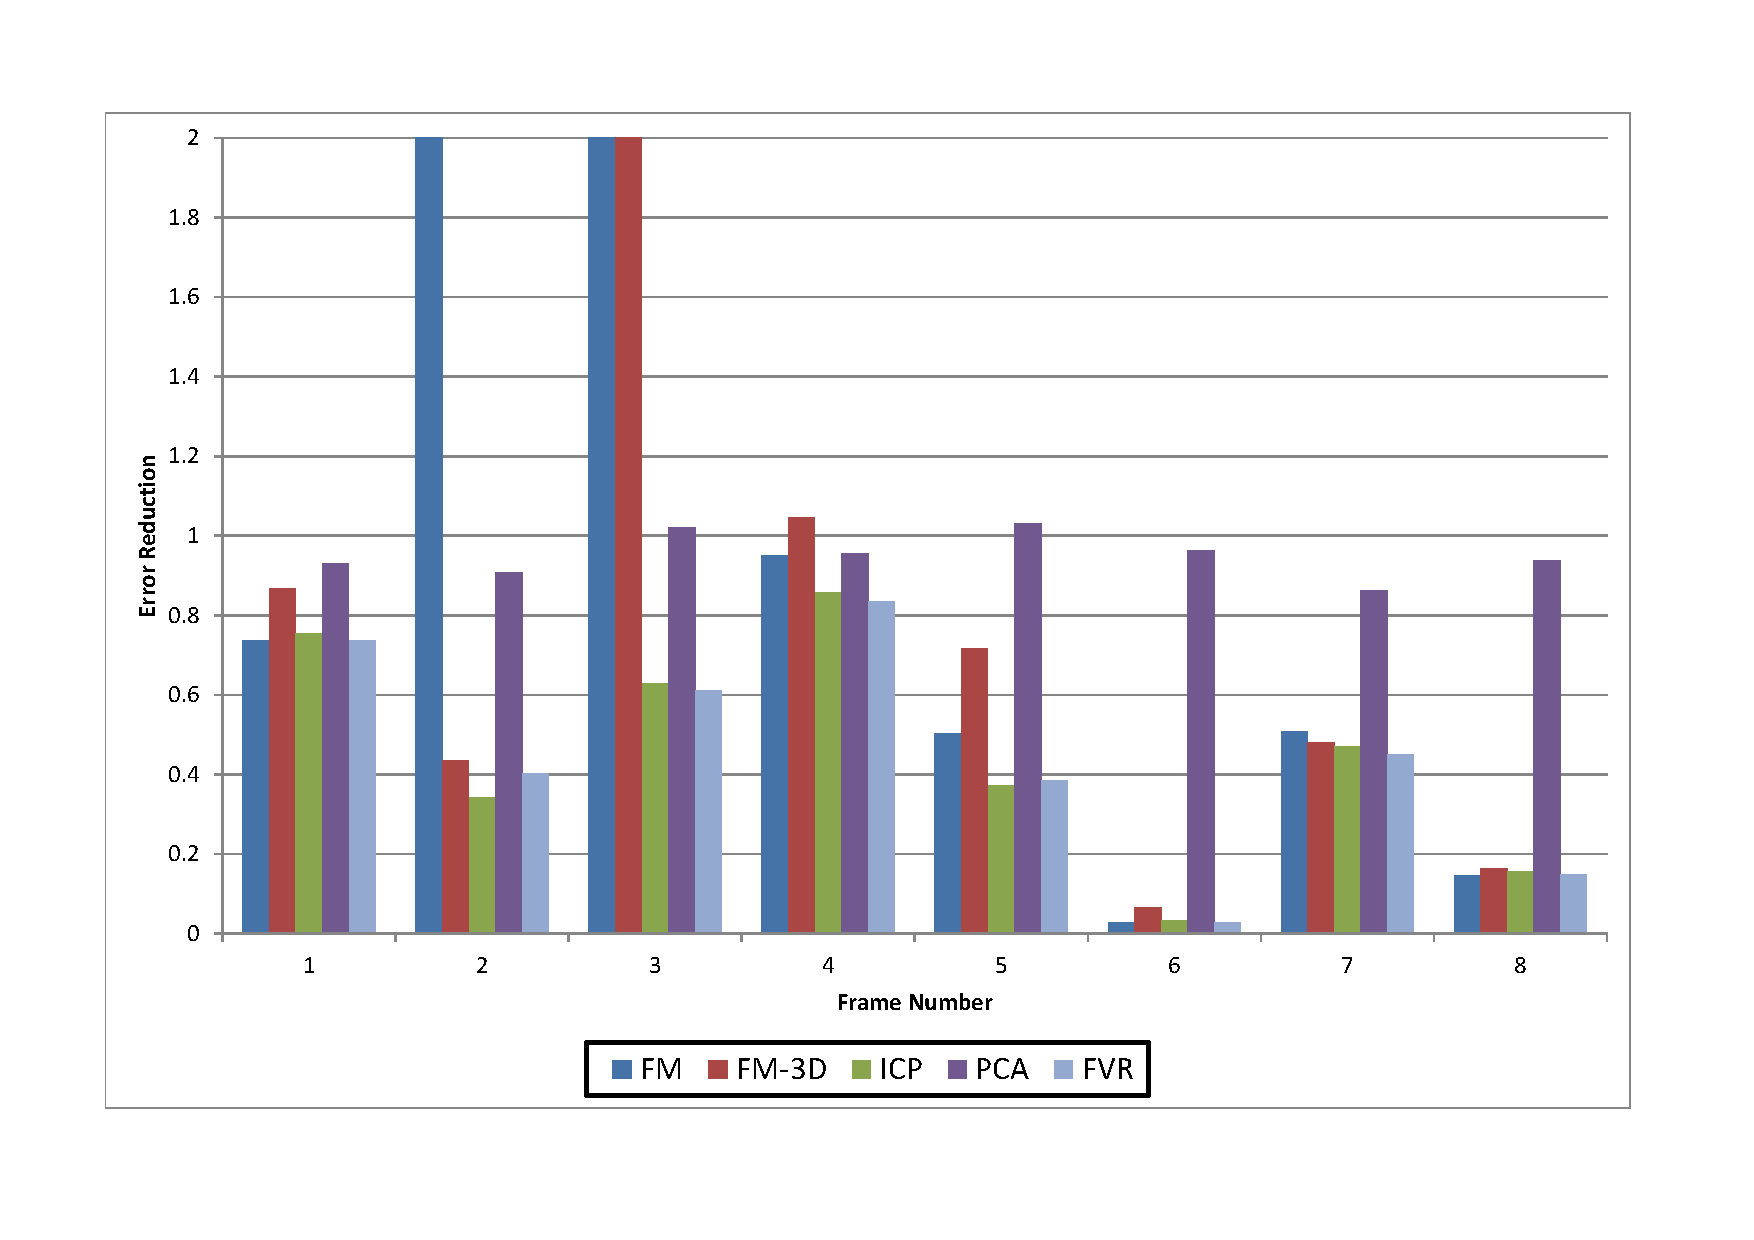
\includegraphics[width=6.0in]{images/results/Outside_TextureConfusion_Rotation}
\caption{Registration Error for the Outdoors Texture Confusion Rotation Data Set}
\label{fig:PET15}
\end{figure*}

Another test was performed with an outdoors scene. Here only 8 of the frames had any good results for all algorithms. They are shown in figure \ref{fig:PET15}. In these results, 6 out of the 8 frames had either a matching or best registration for the FVR method. 2D-feature-matching and 3D-feature-matching both failed a few times, and PCA was inconsistent. ICP had a competitive result 3 out of the 8 times, both FVR and ICP were most consistent. 

\begin{figure*}[t]
\centering
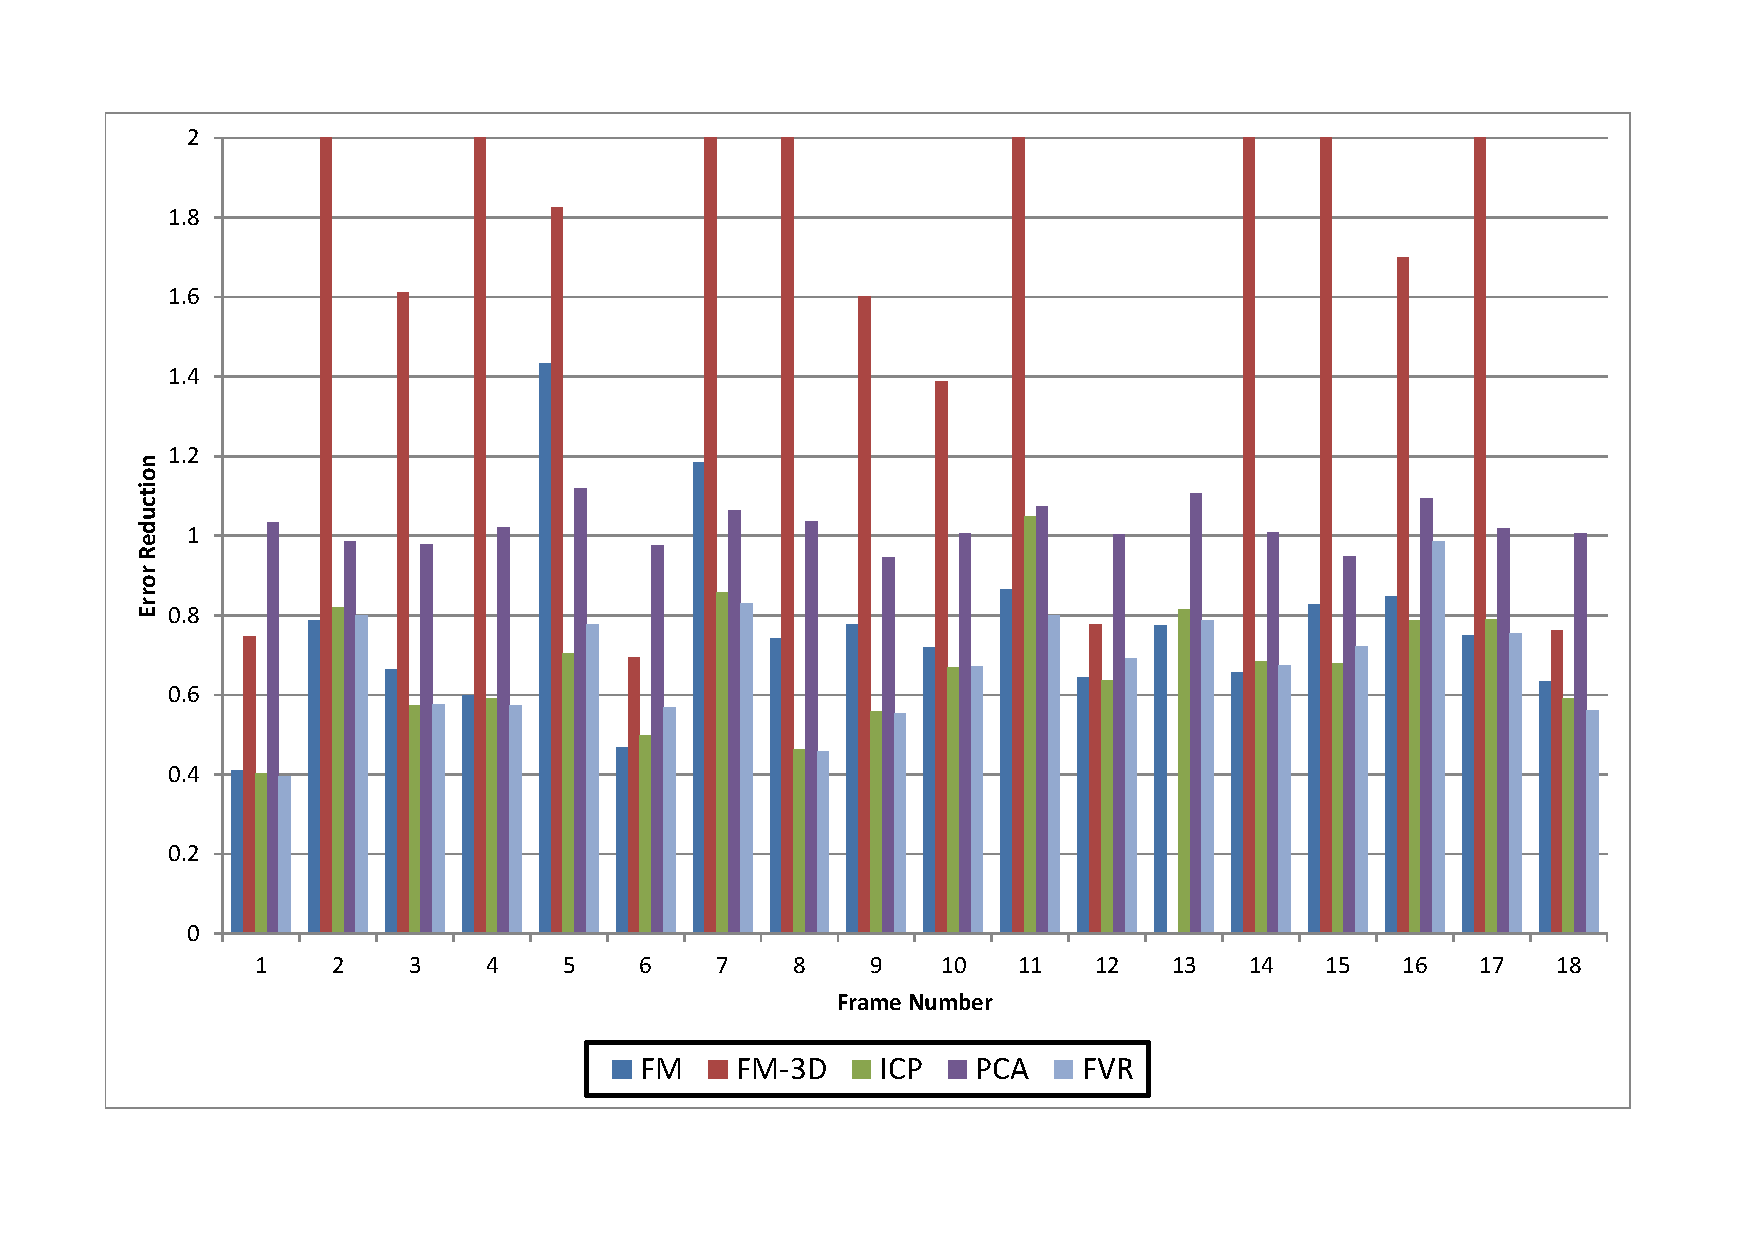
\includegraphics[width=6.0in]{images/results/Outside_TextureConfusion_Translation}
\caption{Registration Error for the Outdoors Texture Confusion Translation Data Set}
\label{fig:PET16}
\end{figure*}

Another scene with texture-confusion was taken out-doors. The interesting results are shown in figure \ref{fig:PET16}. Here, 3D-feature matching failed a majority of the time. Interestingly PCA also failed, the likely reason is because of the amount of noise in an out-doors scene. This noise can give inconsistencies in the principal axes and mean computation. Again, FVR performed best with it getting the best or equivalent result around 55\% of the time. This is another experiment where FVR is shown to be highly robust to scenes with texture confusion. 

\begin{figure*}[t]
\centering
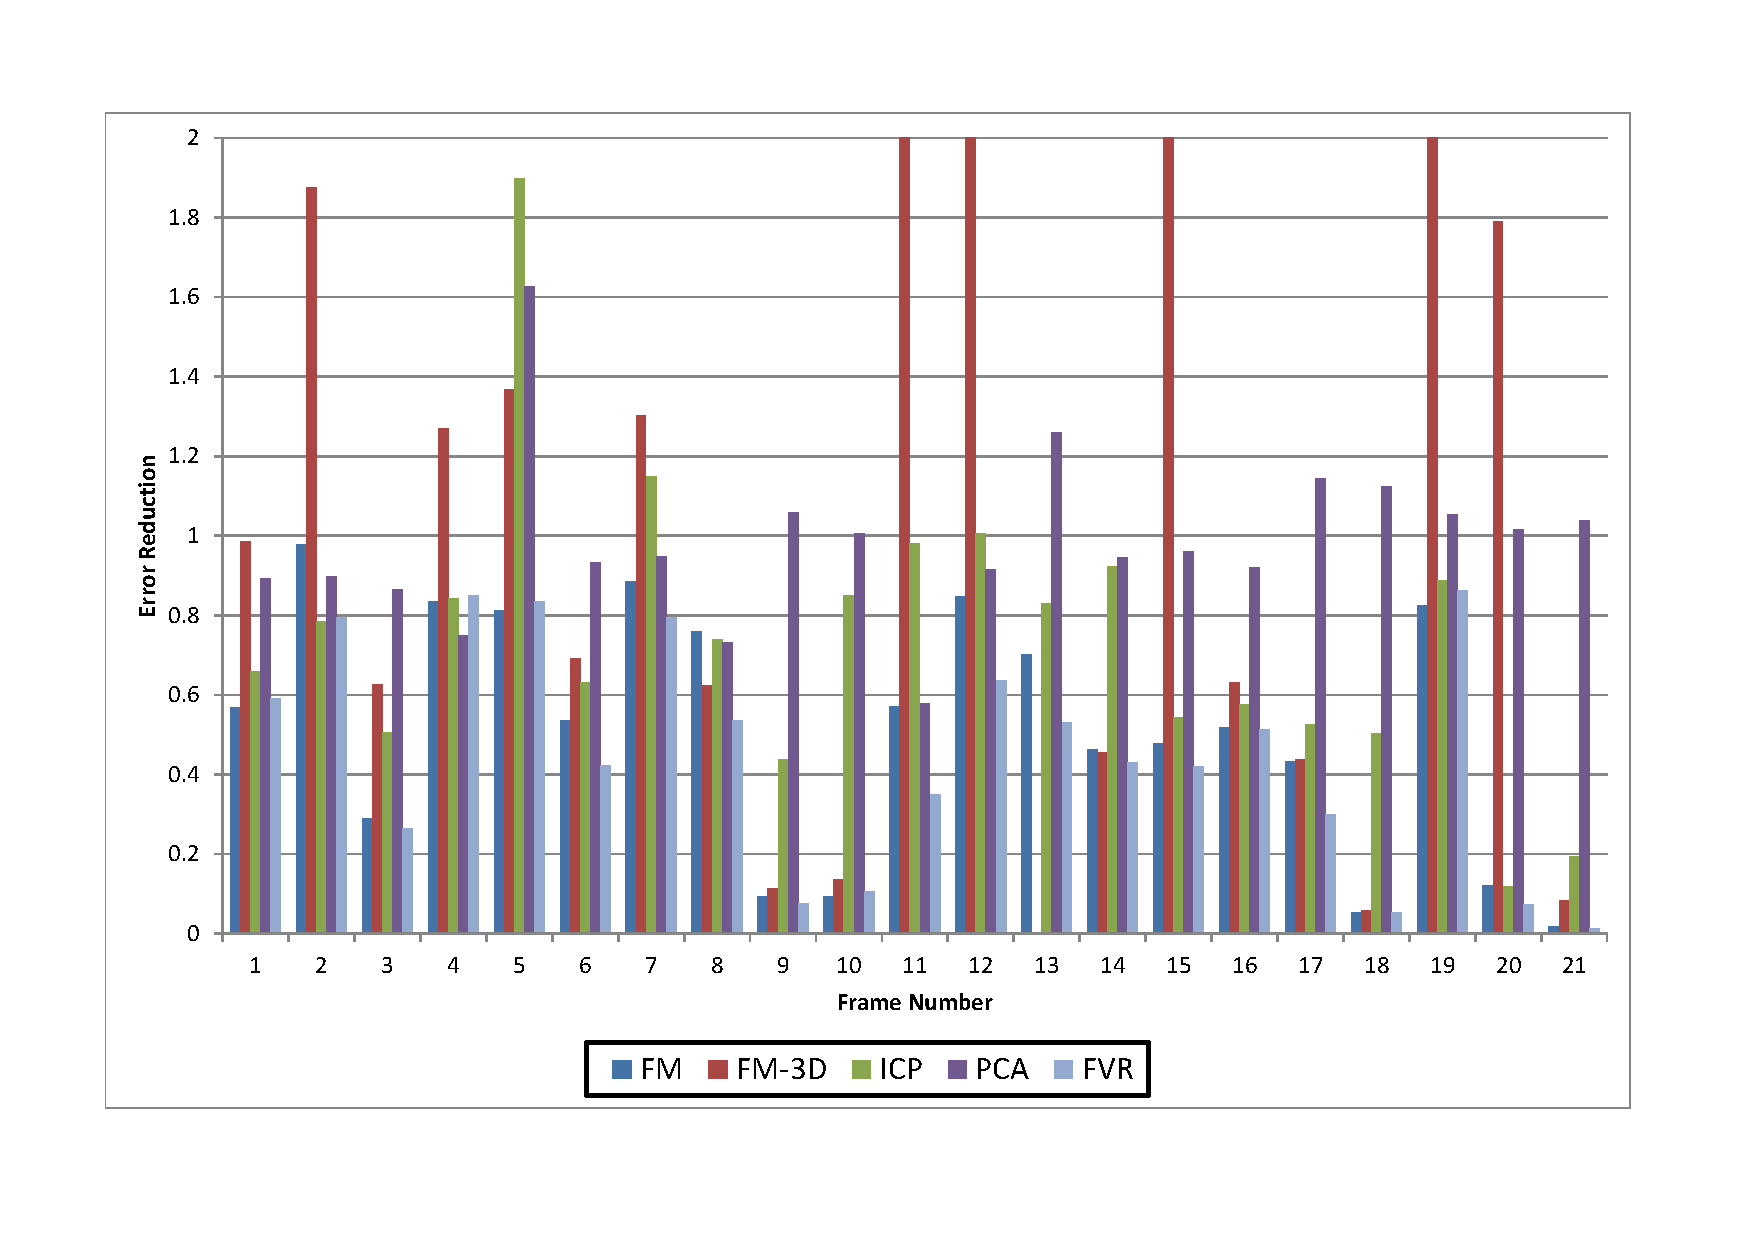
\includegraphics[width=6.0in]{images/results/Plants_Outdoors_Texture_Confusion_Rotation}
\caption{Registration Error for the Outdoor Plants Texture Confusion Rotation Data Set}
\label{fig:PET17}
\end{figure*}

The final figure in the pose estimation tests shows another scene taken out-doors. This scene also contains texture confusion, but the camera was rotated about an axis rather than translated in this data-set. Results shown in figure \ref{fig:PET17} indicate that again FVR dominates with 16 out of the 21 frames having a matching or best registration by FVR. 


\section{Noise Robustness Experiments}



\subsection{Camera Movement Tests}

In this section, camera parameters found by the FVR method are compared to ground truth data under various levels of noise. The Signal to Noise Ratio (SNR) metric is used to describe the noise added to the data prior to registration. A noise value of $x$\% means random noise was added in the range [$-0.5x$, $0.5x$]. Camera registration error is measured in centimetres and voxel error (the error in the phase correlation volume). Table \ref{table:trans} shows the FVR's robustness to noise whilst the camera was moved at different intervals. Results indicate that for camera movements of up to 15cm and SNR higher than 6.0 the FVR method is robust to noise. In video frame rates, a displacement of 10cm per frame equates to camera velocity of 3 m/s (roughly twice normal walking speed).  \\


%translation
\begin{table}[ht]
\centering
\scalebox{0.75}{
\begin{tabular}{ccccc}
\hline
\textbf{translation (cm)} & \textbf{noise range (\%)} & \textbf{SNR} & \textbf{error (cm)} & \textbf{error (voxel)}\\ \hline
5cm & 0 & $\infty$ & 0 & 0\\
5cm & 10 & 20db & 0 & 0\\
5cm & 25 & 12db & 0 & 0\\
5cm & 50 & 6db & 0 & 0\\
5cm & 75 & 2.5db & 112.28 & 89.83\\
10cm & 0 & $\infty$ & 0 & 0\\
10cm & 10 & 20db & 0 & 0\\
10cm & 25 & 12db & 0 & 0\\
10cm & 50 & 6db & 156.65 & 125.32\\
15cm & 0 & $\infty$ & 2.8 & 2.24\\
15cm & 10 & 20db & 2.8 & 2.24\\
15cm & 25 & 12db & 2.8 & 2.24\\
15cm & 50 & 6db & 198.55 & 158.84\\
\\
\end{tabular}}
\\
\caption{Translation Tracking}
\label{table:trans}
\end{table}[ht]


Table \ref{table:rote} shows results for camera rotation experiments. Degrees of separation tested include: 10, 20 and 30 degrees. Twelve degrees per frame is almost a full rotation per second in video rates. Given 10 degrees of separation, the error was below 1 degree for noise levels less than or equal to 30\%. This base line error is due to the sampling resolution of the volume, as voxel error was in fact zero. As with pure translation, the effect of noise increases with camera disparity. At 30 degrees, little matching information is available. However, for noise levels of 10\% or less, voxel distance error was as low as 4 with an angular error less than $3.8$. Rotations of this magnitude are unlikely as motion blur would occur.



\begin{table*}[ht]
\parbox{.45\linewidth}{
\centering
\scalebox{0.75}{
\begin{tabular}{ccccc}\hline
\textbf{rotation} & \textbf{noise (\%)} & \textbf{SNR} & \textbf{error ($\theta$)} & \textbf{error (voxel)}\\ \hline
$10^{\circ}$ & 0 & $\infty$ & 0.31 & 0\\
$10^{\circ}$ & 10 & 20db & 0.31 & 0\\
$10^{\circ}$ & 25 & 12db & 0.63 & 1\\
$10^{\circ}$ & 30 & 10.5db & 90.62 & 96\\
$20^{\circ}$ & 0 & $\infty$ & 0.31 & 0\\
$20^{\circ}$ & 10 & 20db & 0.63 & 1\\
$20^{\circ}$ & 15 & 16.5db & 38.13 & 40\\
$30^{\circ}$ & 0 & $\infty$ & 3.75 & 4\\
$30^{\circ}$ & 10 & 20db & 3.28 & 3\\
$30^{\circ}$ & 15 & 16.5db & 30 & 32\\
\\
\end{tabular}}
\caption{Rotation Tracking}
\label{table:rote}
}

\subsection{Object Motion Test}

\hfill
\parbox{.45\linewidth}{
\centering
\scalebox{0.75}{
\begin{tabular}{ccc}\hline
\textbf{Object Size} & \textbf{error (cm)} & \textbf{error (voxel)}\\ \hline
0.35 & 0 & 0\\
2.95 & 0 & 0\\
6.22 & 0 & 0\\
12.28 & 0 & 0\\
19.82 & 0 & 0\\
22.39 & 0 & 0\\
26.09 & 0 & 0\\
31.00 & 0 & 0\\
48.23 & 38.42 & 15\\
74.32 & 113.57 & 44\\
\\
\end{tabular}}
\caption{Object Motion Test}
\label{table:OBJECT_MOVE_EXP}
}
\end{table*}[ht]


To assess robustness to object motion, experiments were conducted by moving the camera backwards along the z-axis by 5cm per frame whilst moving objects were placed in and out of the scene so that they only appear in one of the volumes being registered. Various sized objects including stacks of CDs, large boxes, people and several pieces of furniture were used and are measured by the percentage of the frame they occupy. Results from Table \ref{table:OBJECT_MOVE_EXP} show the proposed method was accurate upto an object size of 31\%, but failed for objects taking up over 48.23\%.

\subsection{Noise Robustness Comparisons}

Here we present results for noise robustness experiments. Tests were performed by transforming data by various transforms, and adding different amounts of noise. Noise here is measured in both SNR and noise range. A noise range of 1.0 means random noise within the range [$-0.5$, $0.5$] was added. SNR is measured in decibels. 

\begin{figure*}[t]
\centering
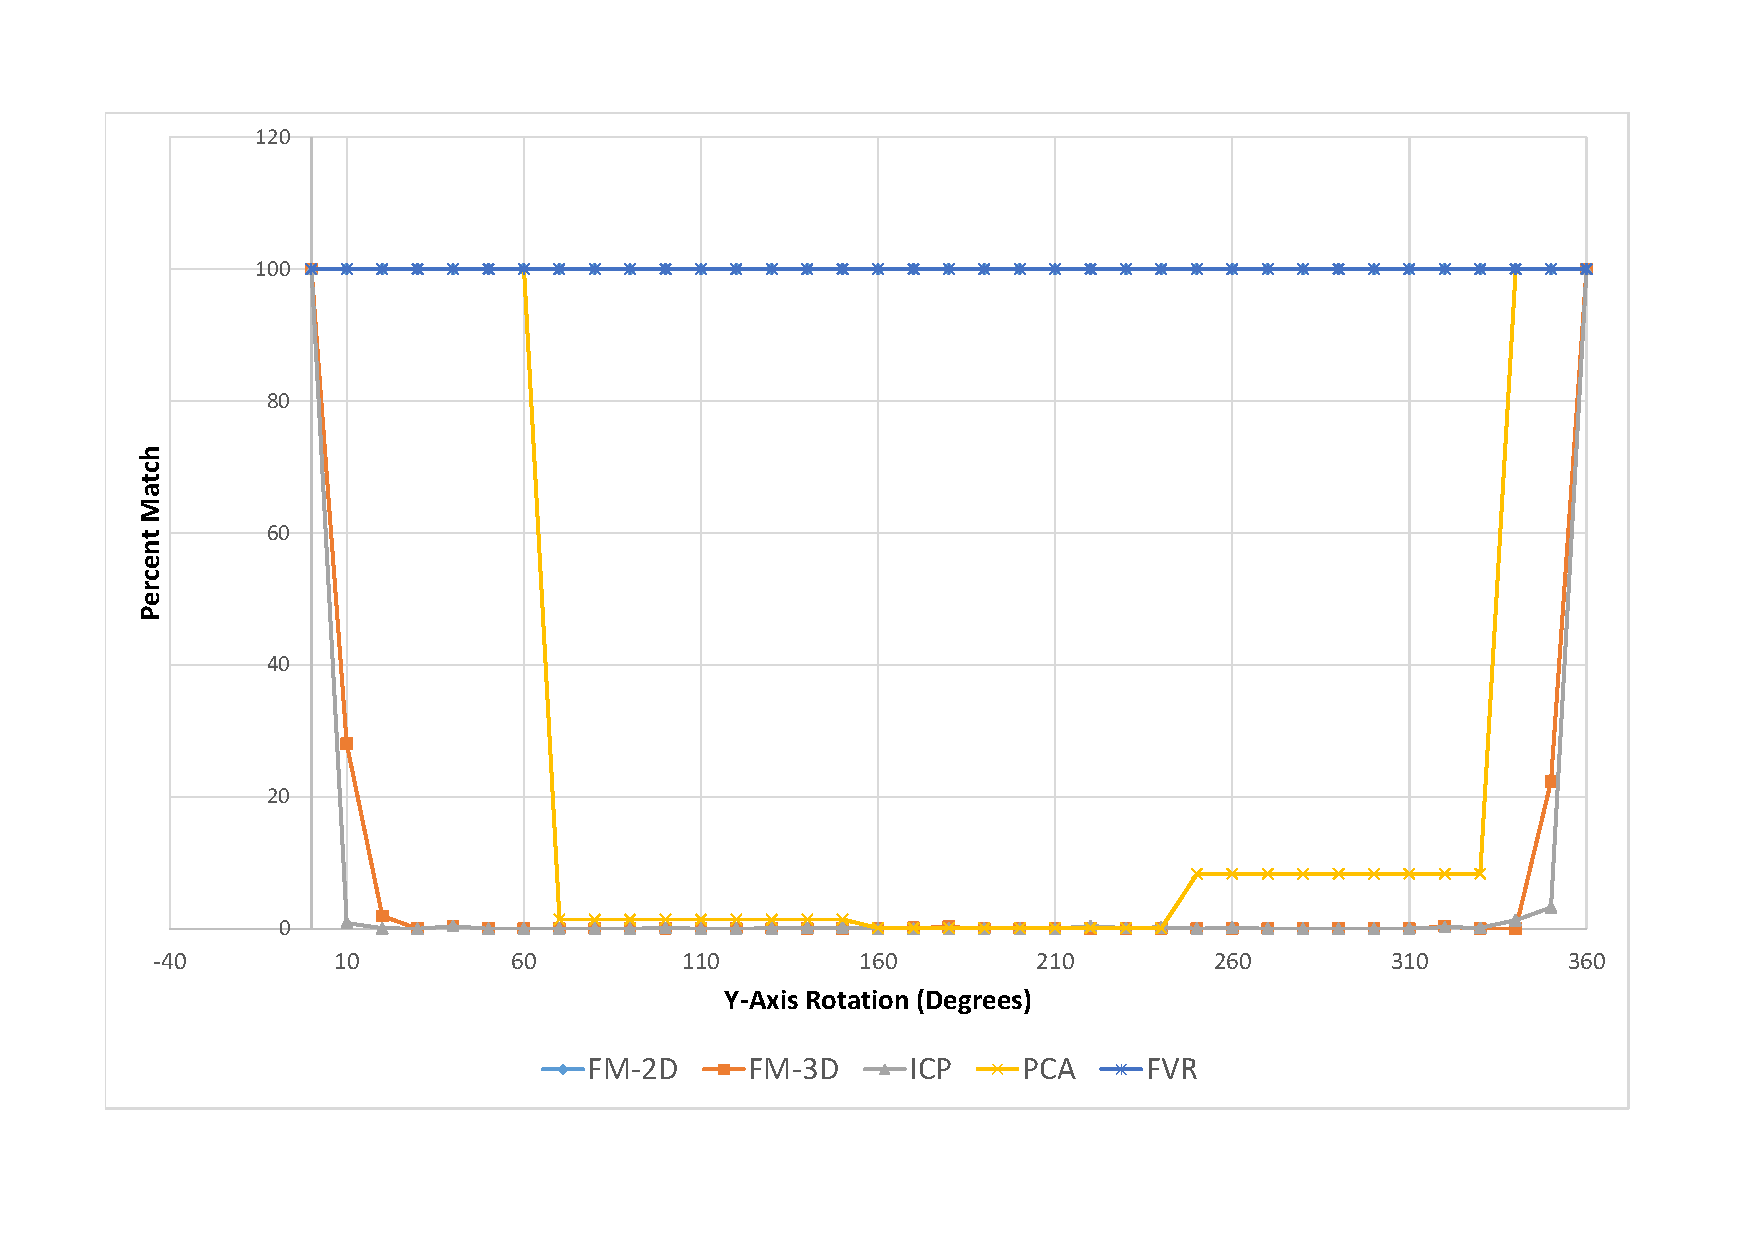
\includegraphics[width=6.0in]{images/results/noise/YRNoise0}
\caption{Percent Match for Y-Axis Registration with an Infinite SNR and noise range of $0$.}
\label{fig:YRNoise0}
\end{figure*}

In the first set of experiments, scanned 3D data was rotated about the Y-axis. Figure \ref{fig:YRNoise0} shows results with an infinite SNR. The 2D-FM method and FVR achieved perfect results. PCA performed next best, but failed to register degrees above 70. Since no noise was present, PCA was truly accurate, however some axes were flipped. This may be fixed by testing the data for flipped axes. FM-3D and ICP fell away much earlier. ICP is not good at registering significant transforms and FM-3D also does not perform well as quantization errors are higher since we use volume sizes of $128^3$.

\begin{figure*}[t]
\centering
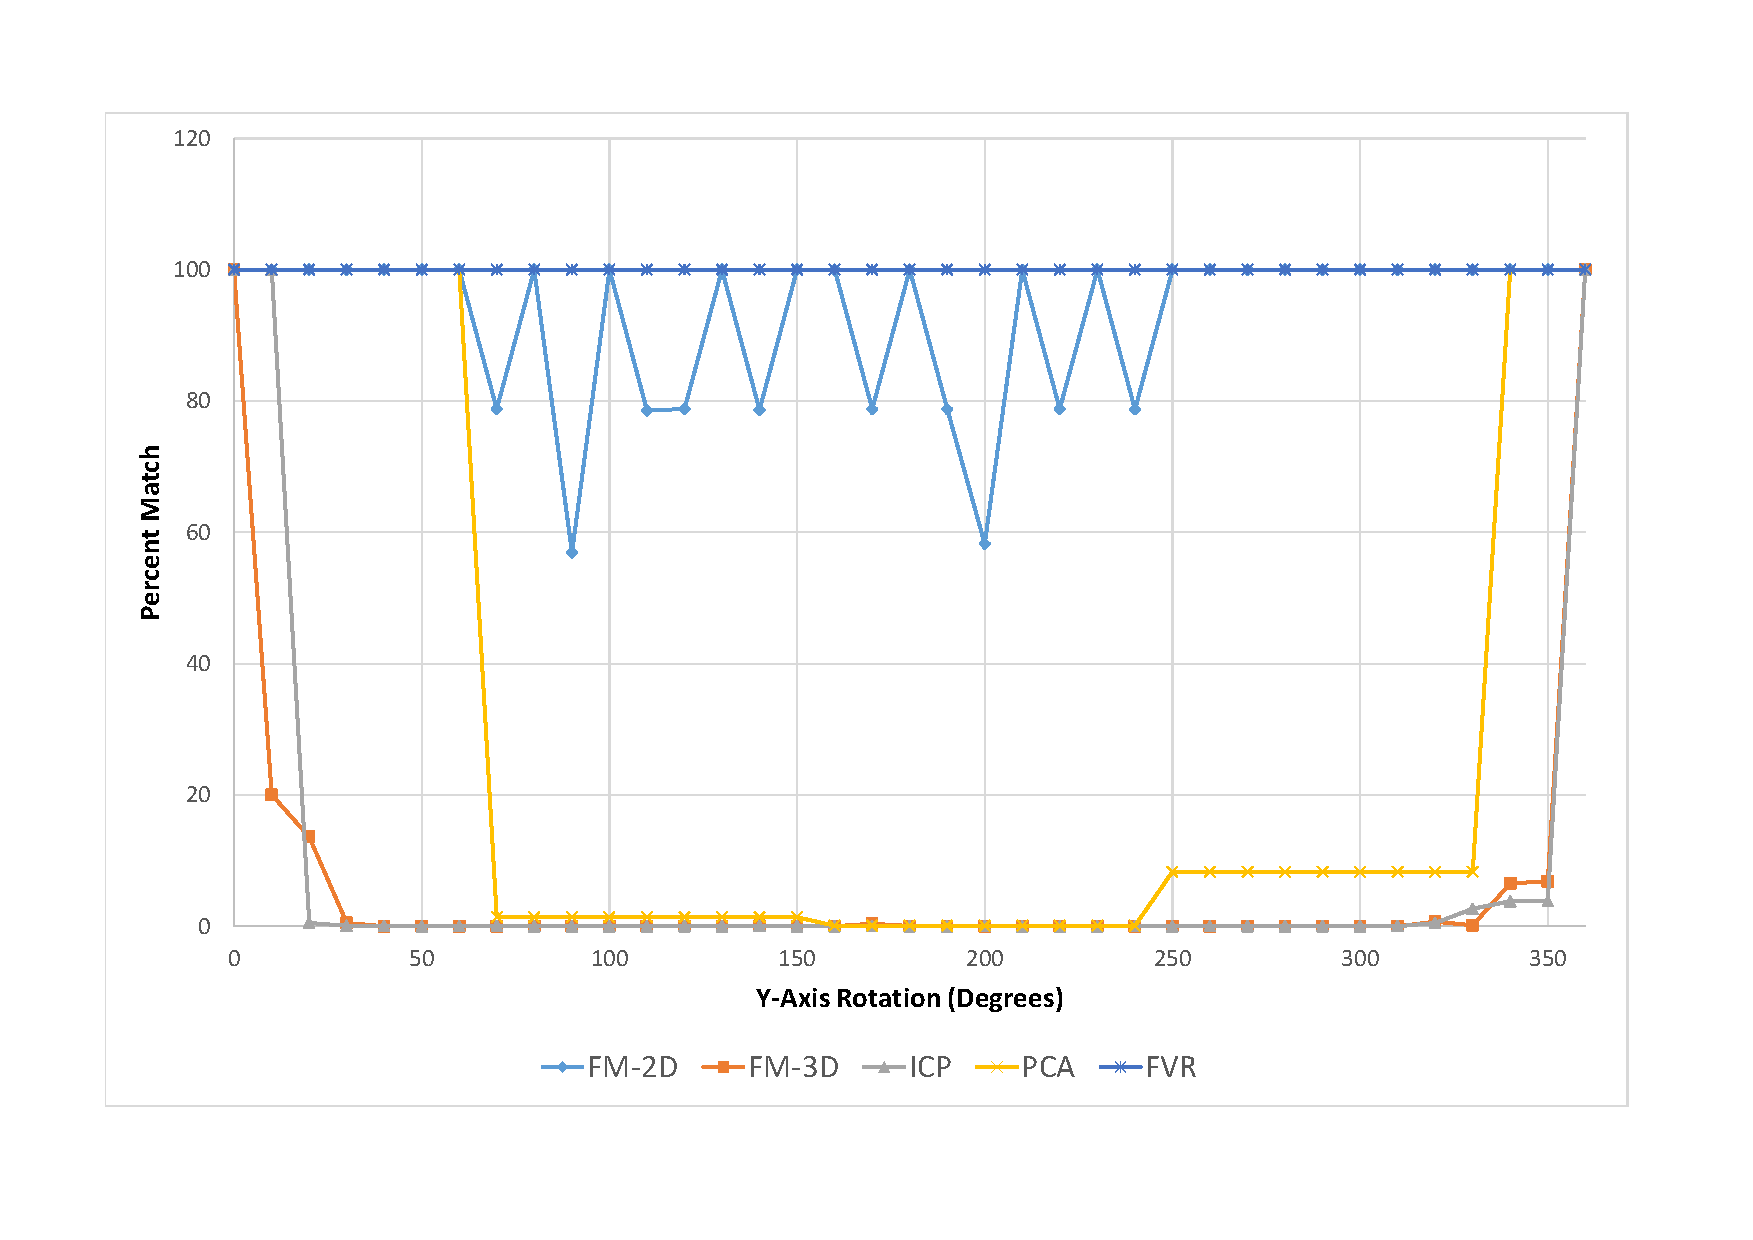
\includegraphics[width=6.0in]{images/results/noise/YRNoise1}
\caption{Percent Match for Y-Axis Registration with an SNR of and noise range of $10300$ and noise range of $1.0$.}
\label{fig:YRNoise1}
\end{figure*}

For the results in figure \ref{fig:YRNoise1} we dropped the SNR to $10300$. Here we see similar results but FM-2D has begun to show some errors with larger rotations (remember rotations above 180 can be considered smaller but negative rotations). In figure \ref{fig:YRNoise2} we reduced the SNR to $2580$ which caused more error in FM-2D. These results suggest that for simple Y-axis rotation, FVR is superior in terms of noise robustness. 

\begin{figure*}[t]
\centering
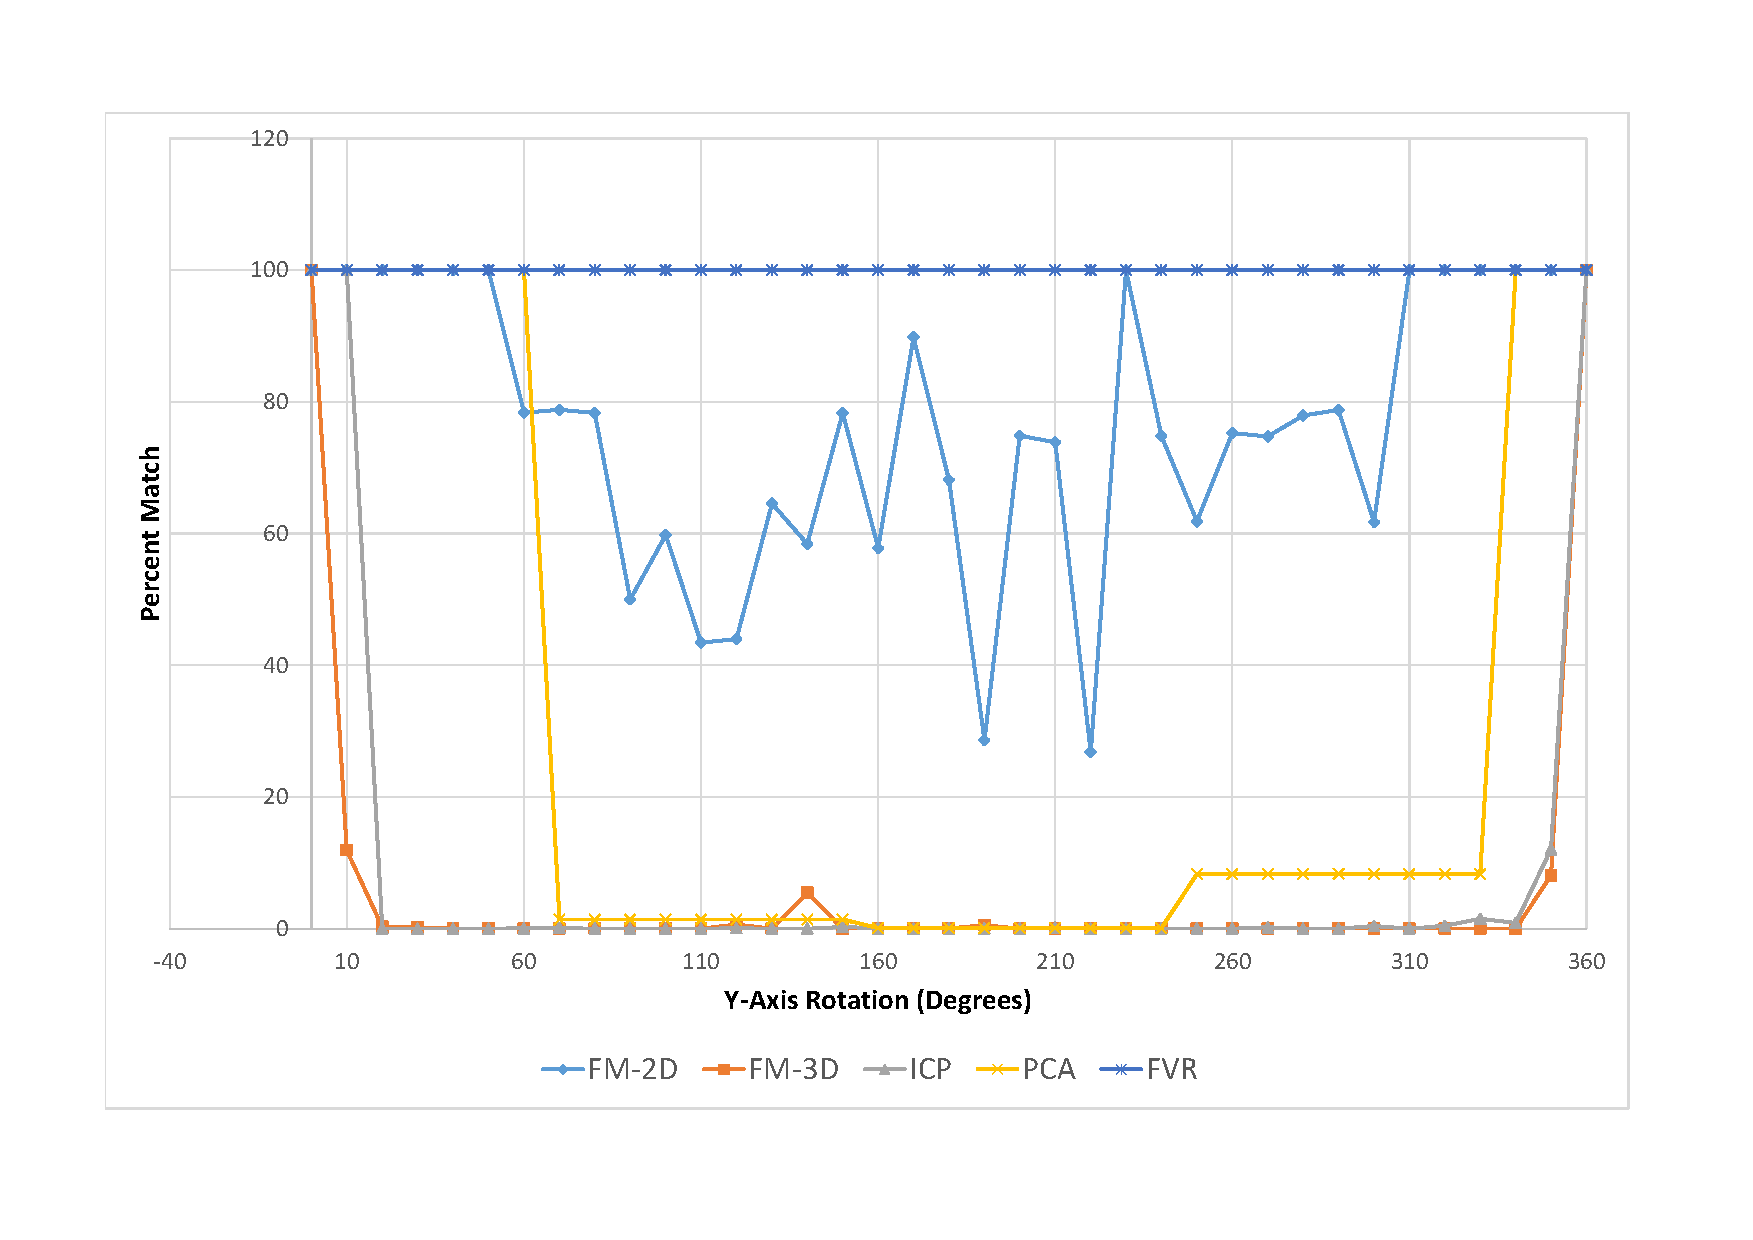
\includegraphics[width=6.0in]{images/results/noise/YRNoise2}
\caption{Percent Match for Y-Axis Registration with an SNR of 2580 and noise range of $2.0$.}
\label{fig:YRNoise2}
\end{figure*}


\begin{figure*}[t]
\centering
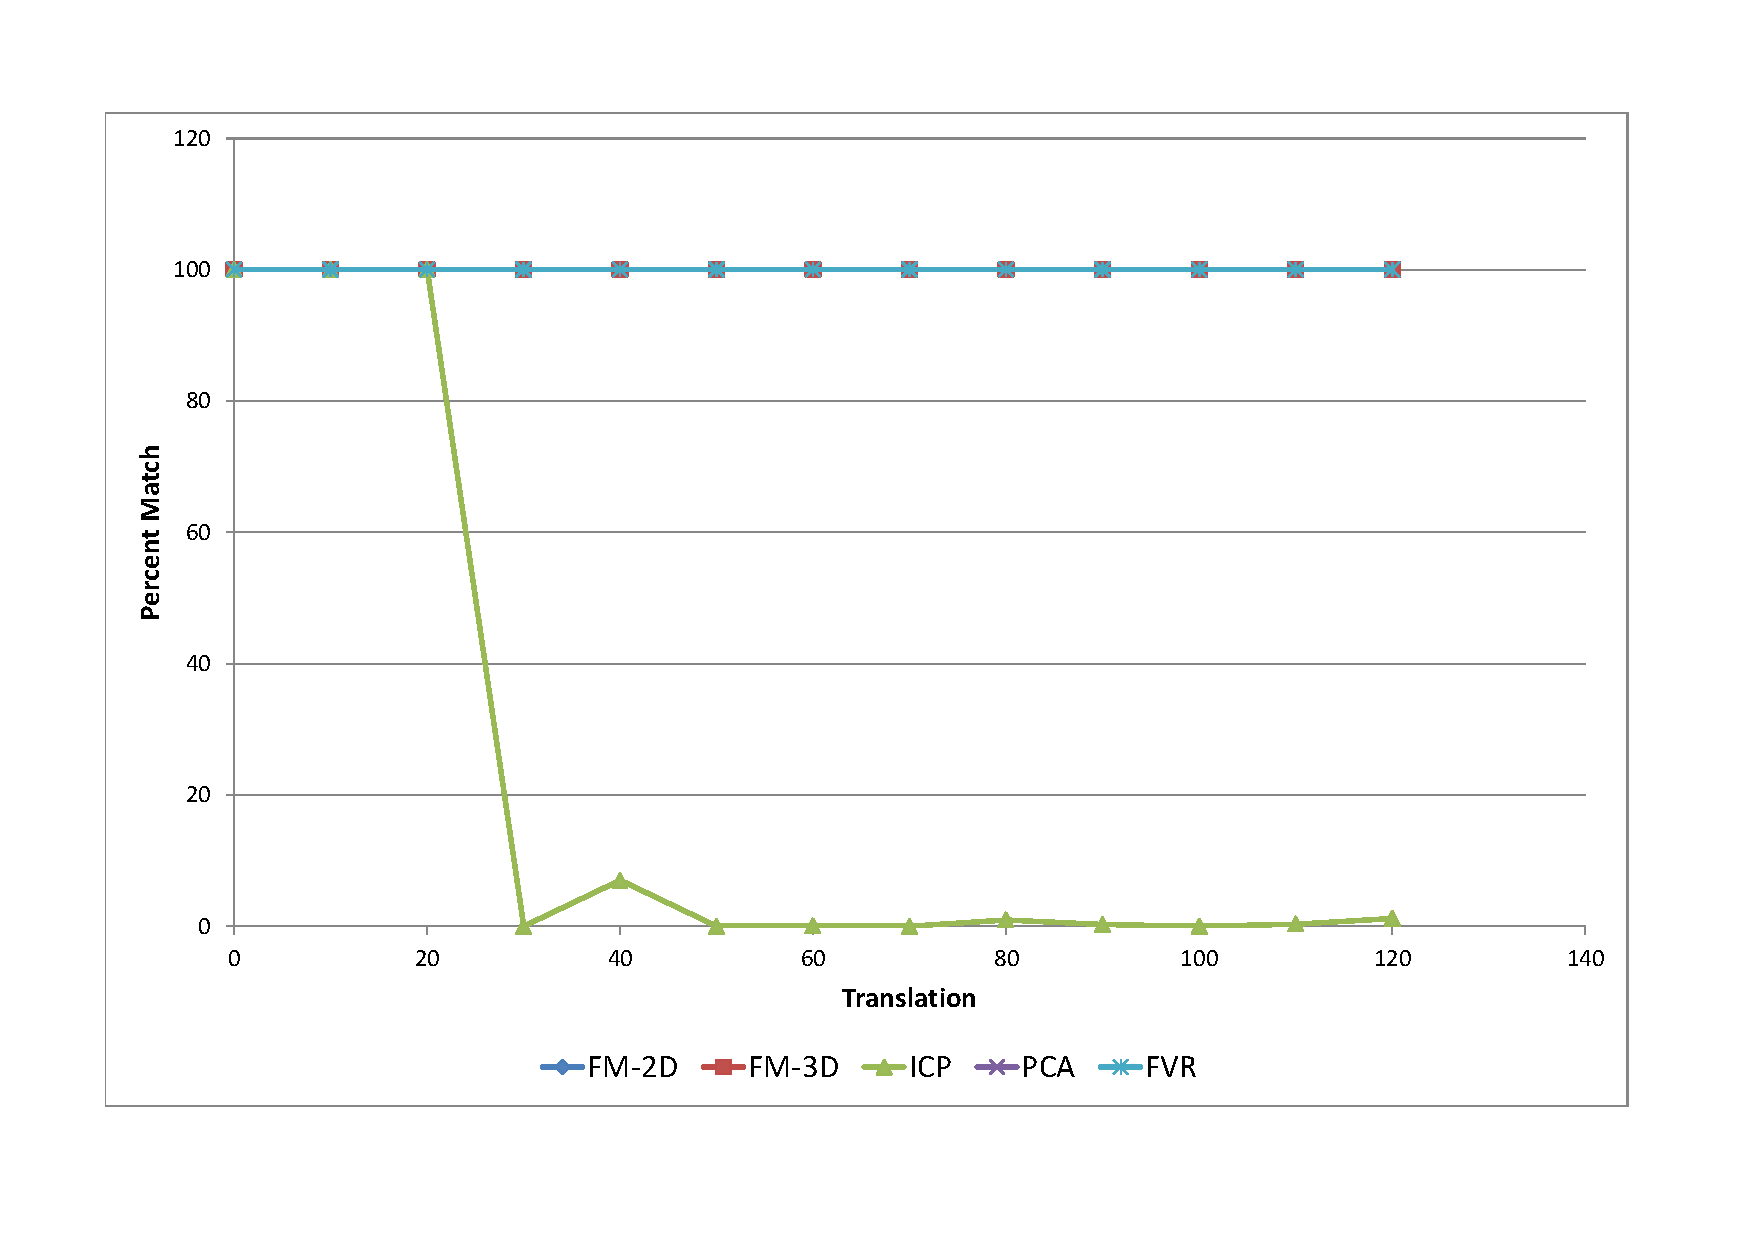
\includegraphics[width=6.0in]{images/results/noise/TransNoise0}
\caption{Percent Match for Translation Registration with an infinite SNR and noise range of $0$.}
\label{fig:TNoise0}
\end{figure*}


\begin{figure*}[t]
\centering
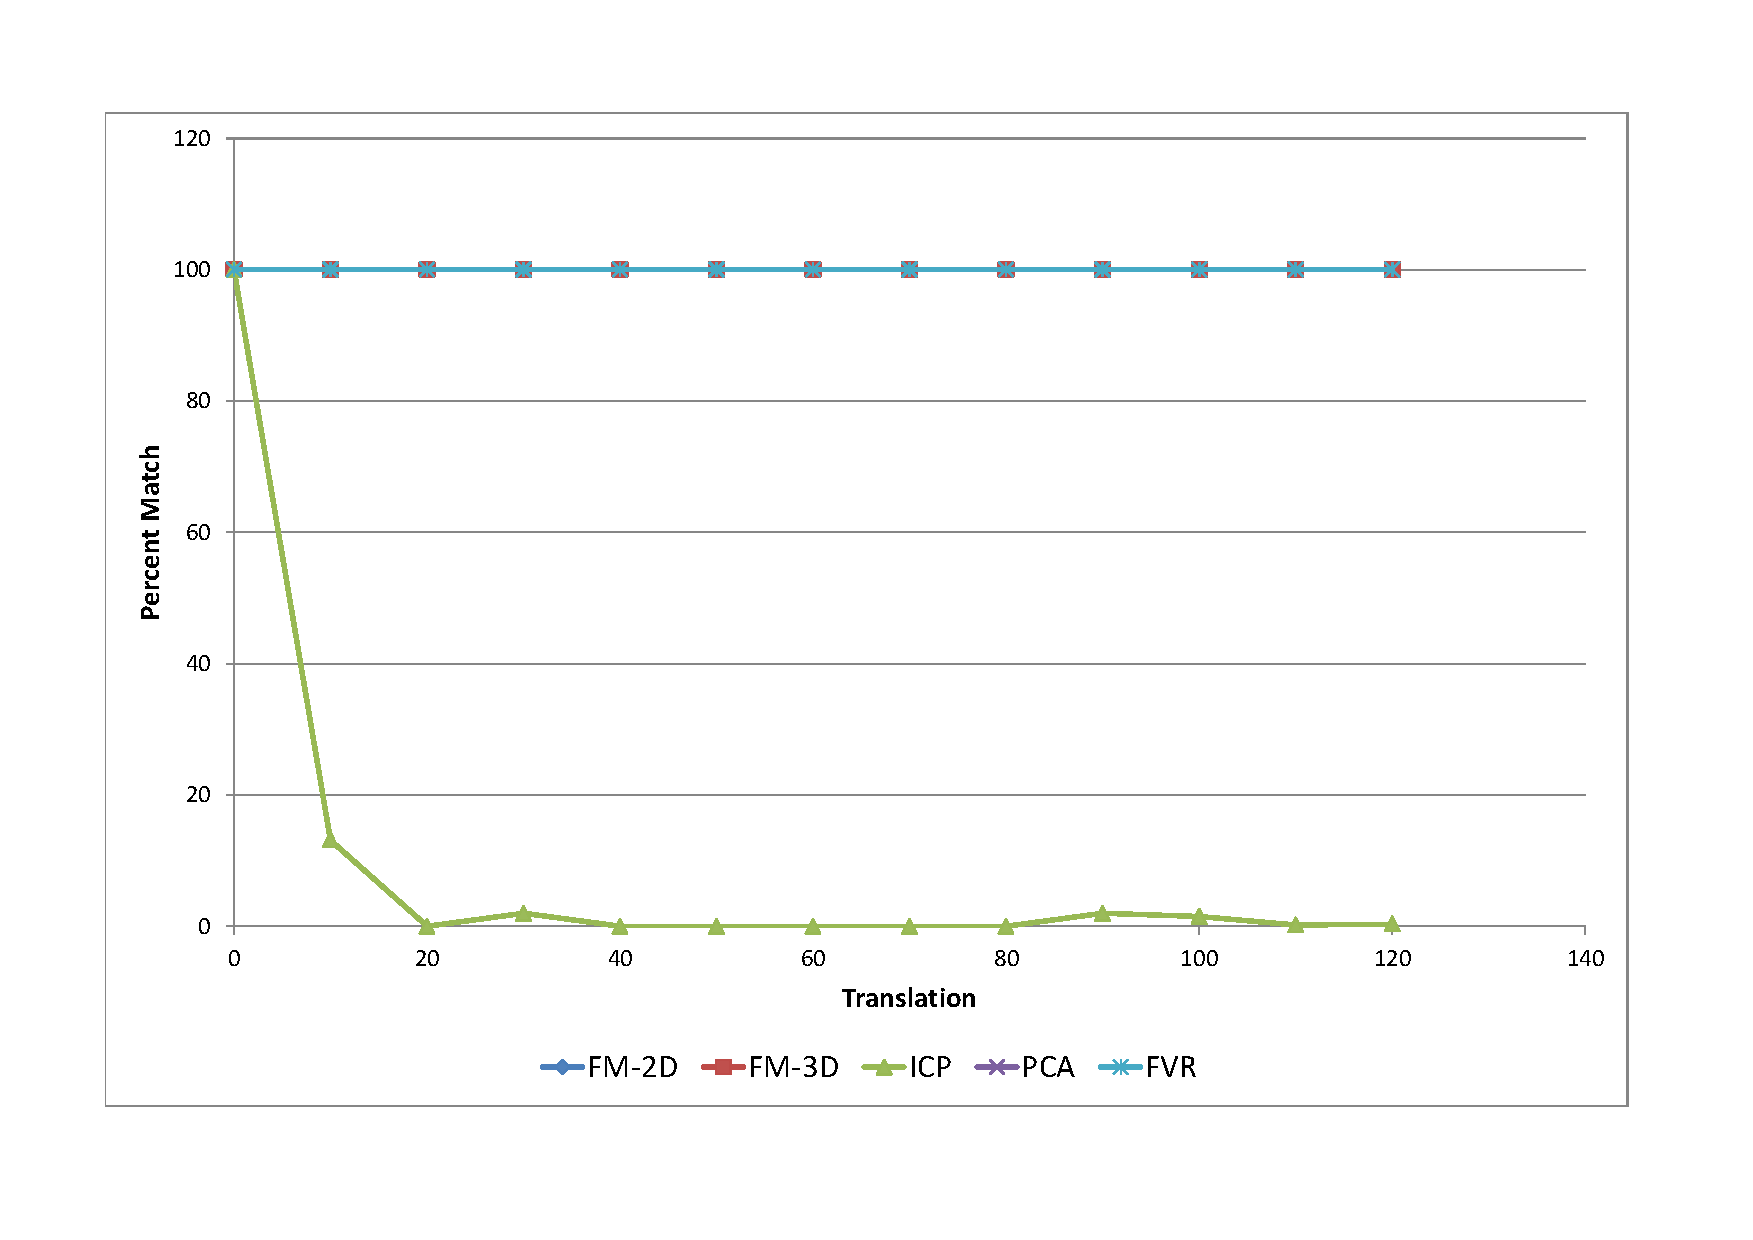
\includegraphics[width=6.0in]{images/results/noise/TransNoise1}
\caption{Percent Match for Translation Registration with an SNR of and noise range of $10300$ and noise range of $1.0$.}
\label{fig:TNoise1}
\end{figure*}


\begin{figure*}[t]
\centering
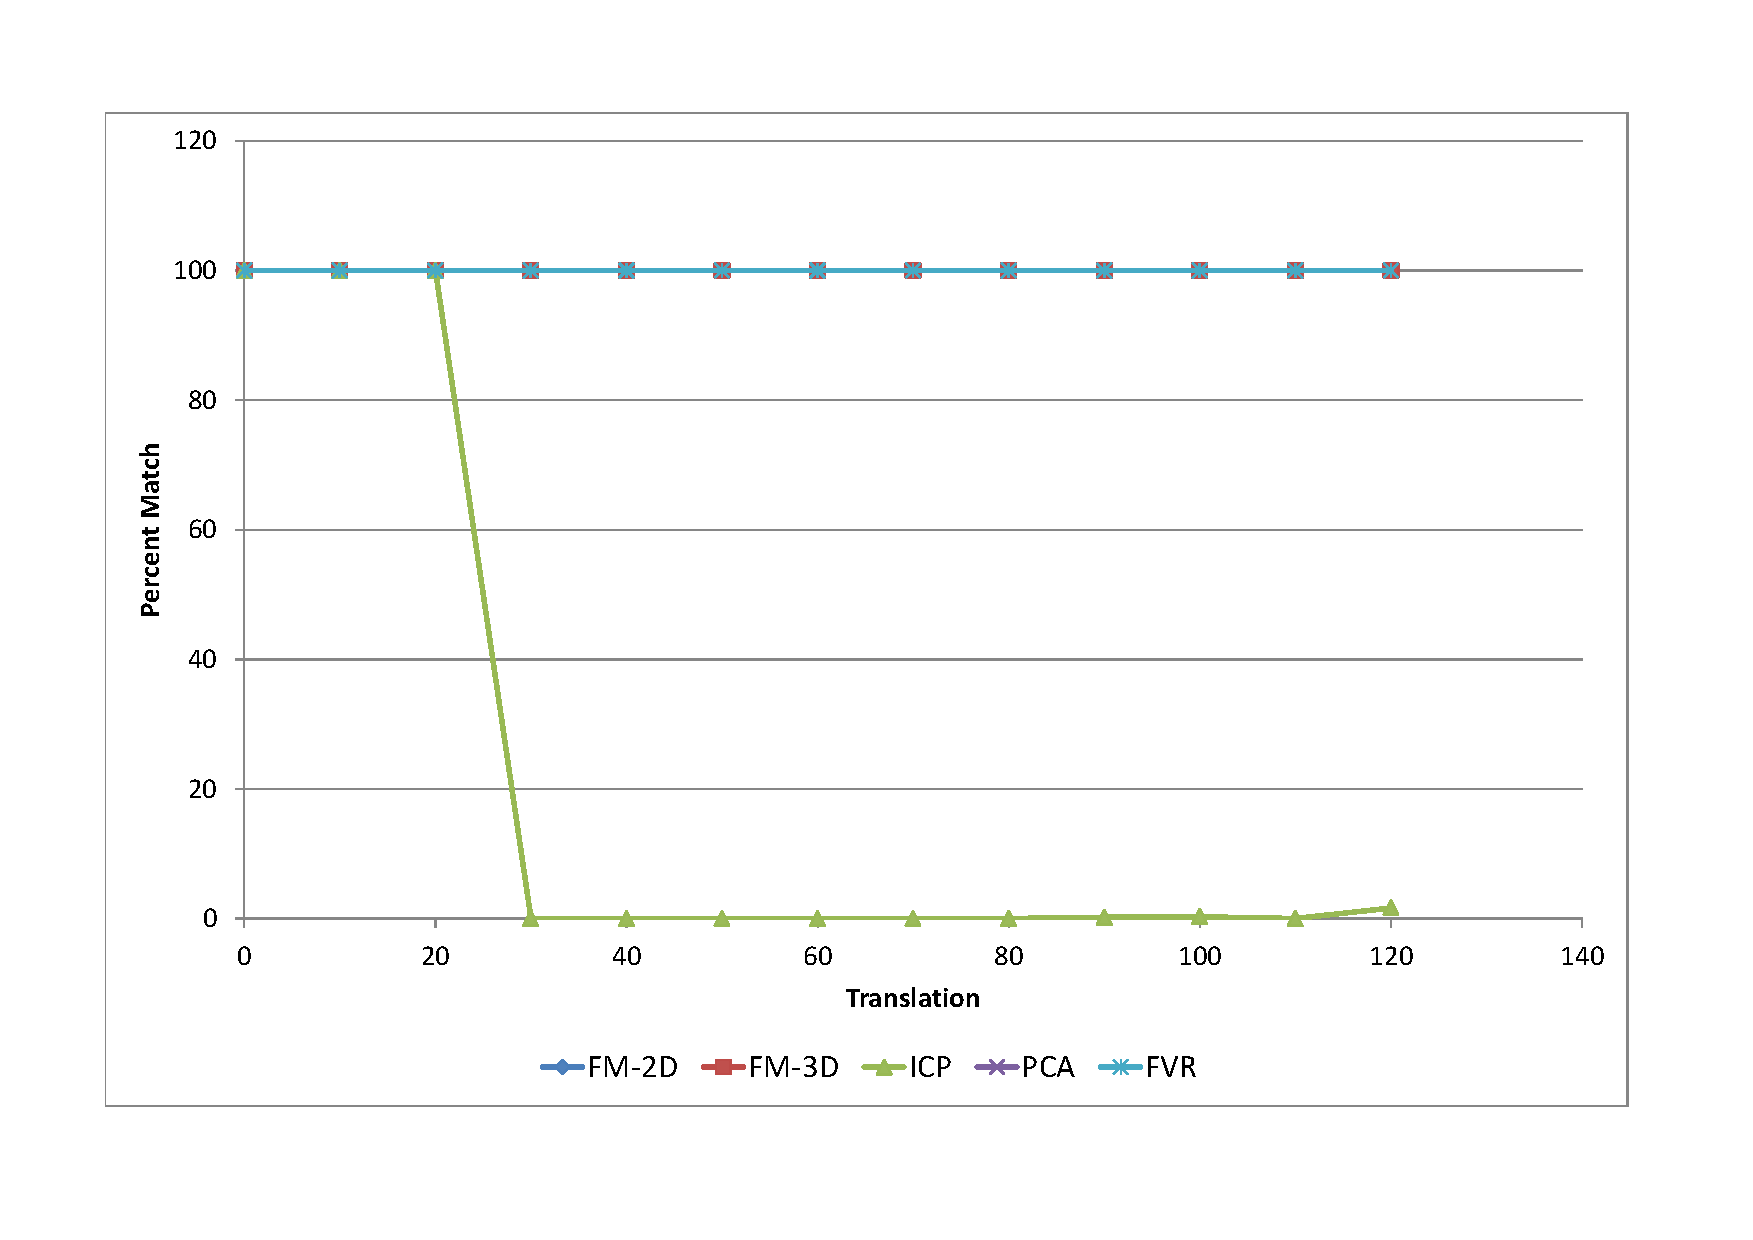
\includegraphics[width=6.0in]{images/results/noise/TransNoise2}
\caption{Percent Match for Translation Registration with an SNR of and noise range of $2580$ and noise range of $2.0$.}
\label{fig:TNoise2}
\end{figure*}







\section{3D Phase Correlation Performance}

The performance of the FVR method is shown theoretically in this section. The size of the volumes being registered is defined as $N^3$ and each frame is sampled at a resolution of $W$ $\times$ $H$. The projection process requires $12WH$ operations whilst re-sampling the point cloud requires $2WH$ operations. The Volume Registration process, $VolumeRegister{\theta \varphi t_x t_y t_z}(V_1, V_2)$ consists of 2 $\times$ Hanning windowing processes, 2 $\times$ 3D FFTs, 2 $\times$ volume-logs, 2 $\times$ log-spherical transforms, 2 $\times$ phase correlation processes and 1 $\times$ linear transformation and peak finding. 

The Hanning windowing function requires 26 operations. The 3D FFT has complexity of $3N^3\log{N}$, the log and log-spherical transform functions require 3 and 58 operations per voxel respectively. Multiplying two frequency spectra together and transforming a volume requires 15 and 30 operations per voxel respectively. Finding the peak value requires $2N^3$ operations. The complexity in terms of number of operations for the phase correlation process is given in Eq. \ref{eqn:PCFULLPERFORMANCE} This process requires 2 $\times$ 3D FFTs, 1 $\times$ frequency spectra multiplication, and 1 $\times$ peak finding operation. 
\begin{equation} \label{eqn:PCFULLPERFORMANCE}
6N^3\log{N} + 2N^3 + 15
\end{equation}
The total complexity can then be found by taking into account the projection and re-sampling totals as well as the total for $VolumeRegister{\theta \varphi t_x t_y t_z}(V_1, V_2)$. Tallying the number of operations for each process and multiplying them by number of times the process is performed gives us the number of operations as a function of $W$, $H$ and $N$ in Eq. \ref{eqn:FULLPERFORMANCE}.
\begin{equation} \label{eqn:FULLPERFORMANCE}
6N^3 + 28WH + 18(N^3\log{N}) + 230
\end{equation}

\subsection{Analysis of Speed Improvement}

To compare performance of the generic volume registration method with the speed up, we use the complexity defined in equation \ref{eqn:FULLPERFORMANCE}. Here, we ignore the cost of projecting the depth map. The 3D DFT has complexity $3N^3log(N)$. This is the first step (see figure \ref{fig:PIPELINE3}), the next is the spherical-map transform which is complexity $45N^3$. If processed on the GPU the performance becomes 45 operations per voxel assuming that one voxel is assigned to one unit of processing. A 3D transform is 30 operations per voxel, 2D phase correlation requires 15 operations to multiply the frequency spectra and $2N^2log(N)$ operations to do the 2D FFT. Finally a projection map transform requires 1 operation per voxel. \\

In total, the proposed method requires $2 \times$ 3D FFTs, $2 \times$ spherical-map transforms, $1 \times$ 3D geometrical transformation, $3 \times$ 2D phase correlations and $4 \times$ projection map transforms. The total complexity is added up for all of these functions and given in equation \ref{eqn:FULLPERF2}. \\

\begin{equation} \label{eqn:FULLPERF2}
6log(N)\times (N^3 + N^2) + 169
\end{equation}

Figure \ref{fig:perfComp} provides a visualization of the performance improvement which the proposed method achieves over the original Fourier volume registration approach. It is clear that the proposed method is around 3 times faster
than the original Fourier based volume registration approach. This is due to the reduction in the amount of data to process afforded by the novel spherical-map transform and orthogonal projection methods.

\begin{figure}[t]
\centering
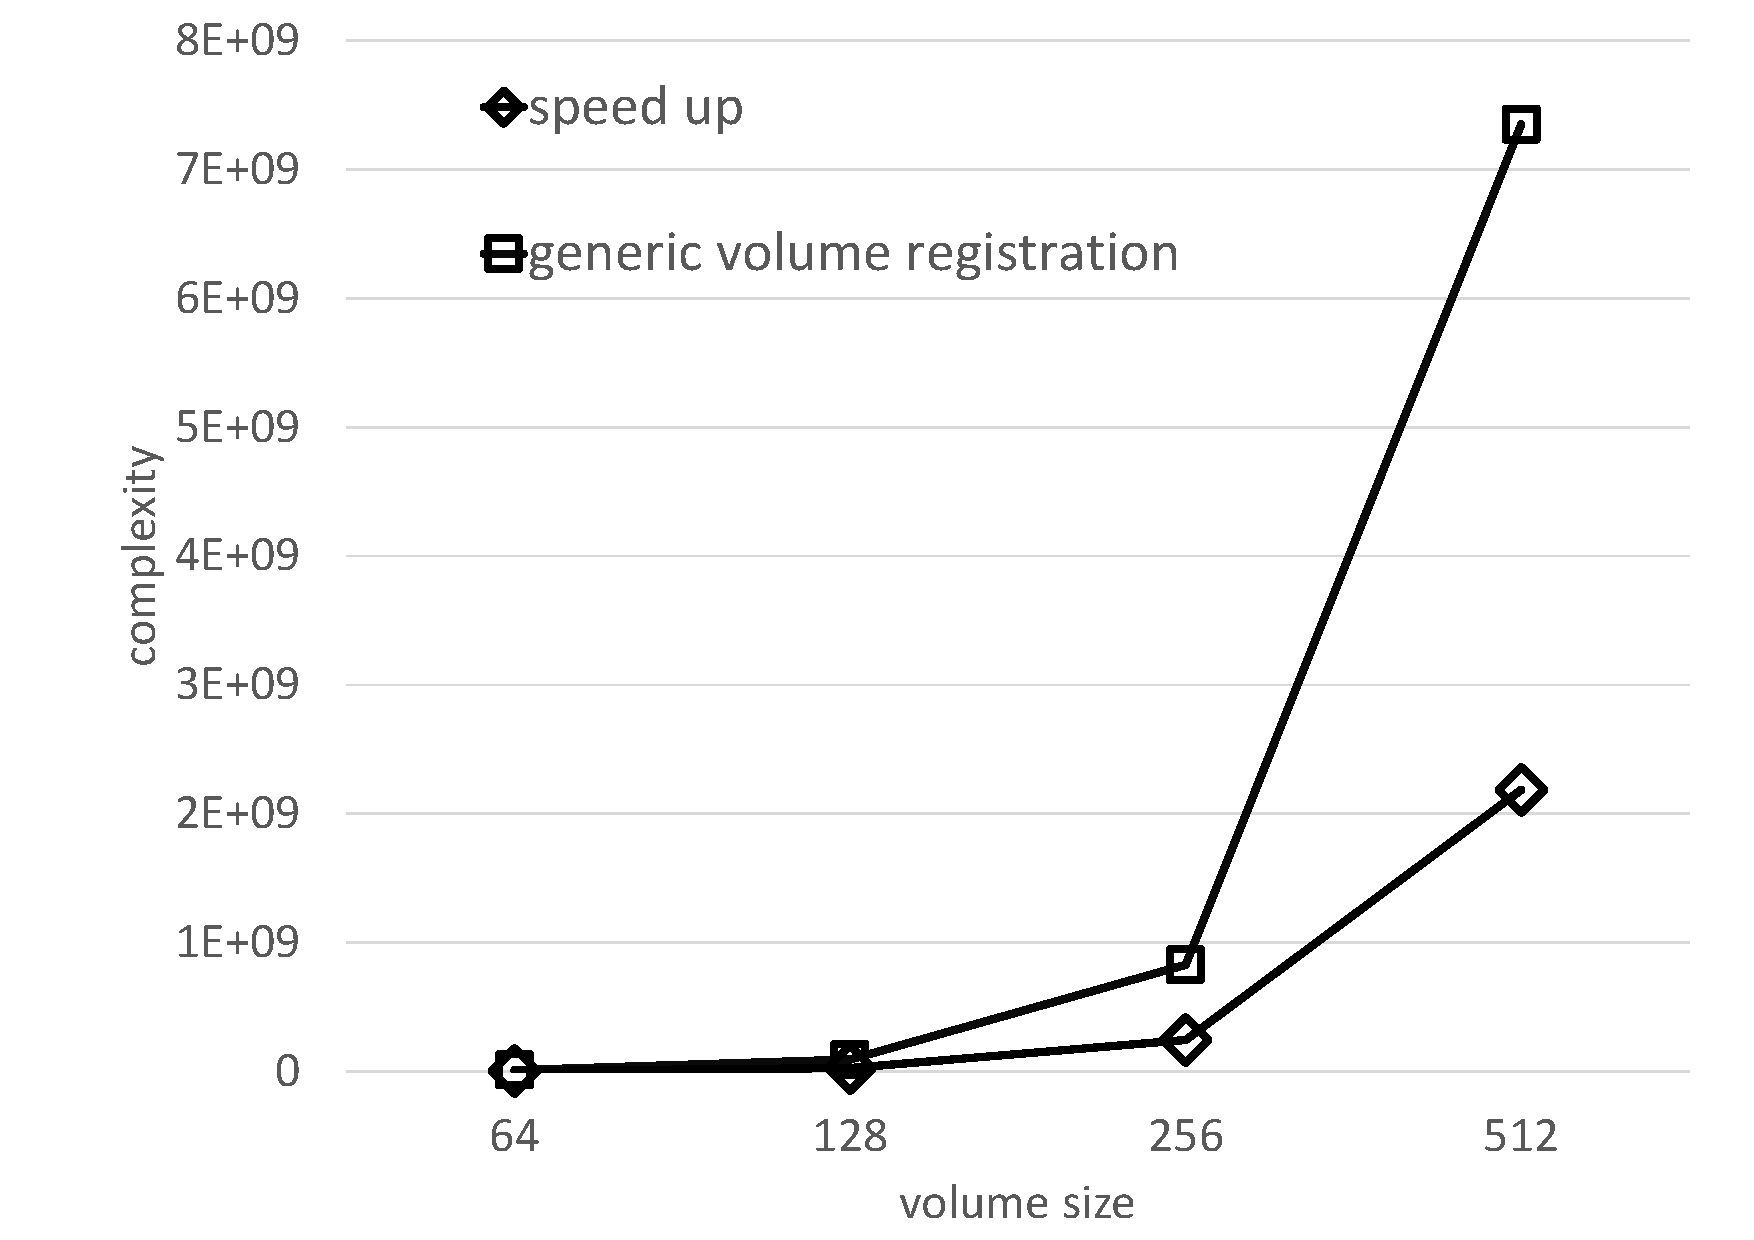
\includegraphics[width=3.0in]{images/results/performance/comparison}
\caption{Comparison of performance between volume registration and the proposed speed up for different volume sizes.}
\label{fig:perfComp}
\end{figure}

\section{Data Representation Experiments}


plane tree is compared with sota mesh compression - proven by my paper published and in terms of compressing 3d reconstructions we compare it to the common OT representation \\

Experiments reveal the Plane-Tree outperforms the original octree and outperforms some state of the art transform methods at low-bitrates. We compare our method with several state of the art algorithms which correspond to transform based methods \cite{Khodakovsky00Progressive,Bayazit103DMesh} and low-bitrate codecs \cite{Peng10Feature}. To compare algorithms quantitatively, we employ rate distortion graphs. Since our algorithm is lossy, this indicates the amount of distortion (in the decoded model compared with the original) given a particular bitrate. To measure distortion, we employ the mean error and root mean squared error, to measure bitrate we use the number of bits per vertex. All measurements are scaled by the main diagonal of the input model. We also provide qualitative results showing the effectiveness of our method. \\

In experiments we use 4 models which are popular amongst researchers in the area. These models are chosen both because they are readily available and because there are available results for these models generated by other state of the art methods. Figure \ref{fig:MODSUSED} shows each model along with its reference name and number of vertices. \\


\begin{figure}[t!] 
        \centering
        \begin{subfigure}[b]{2.8in}
                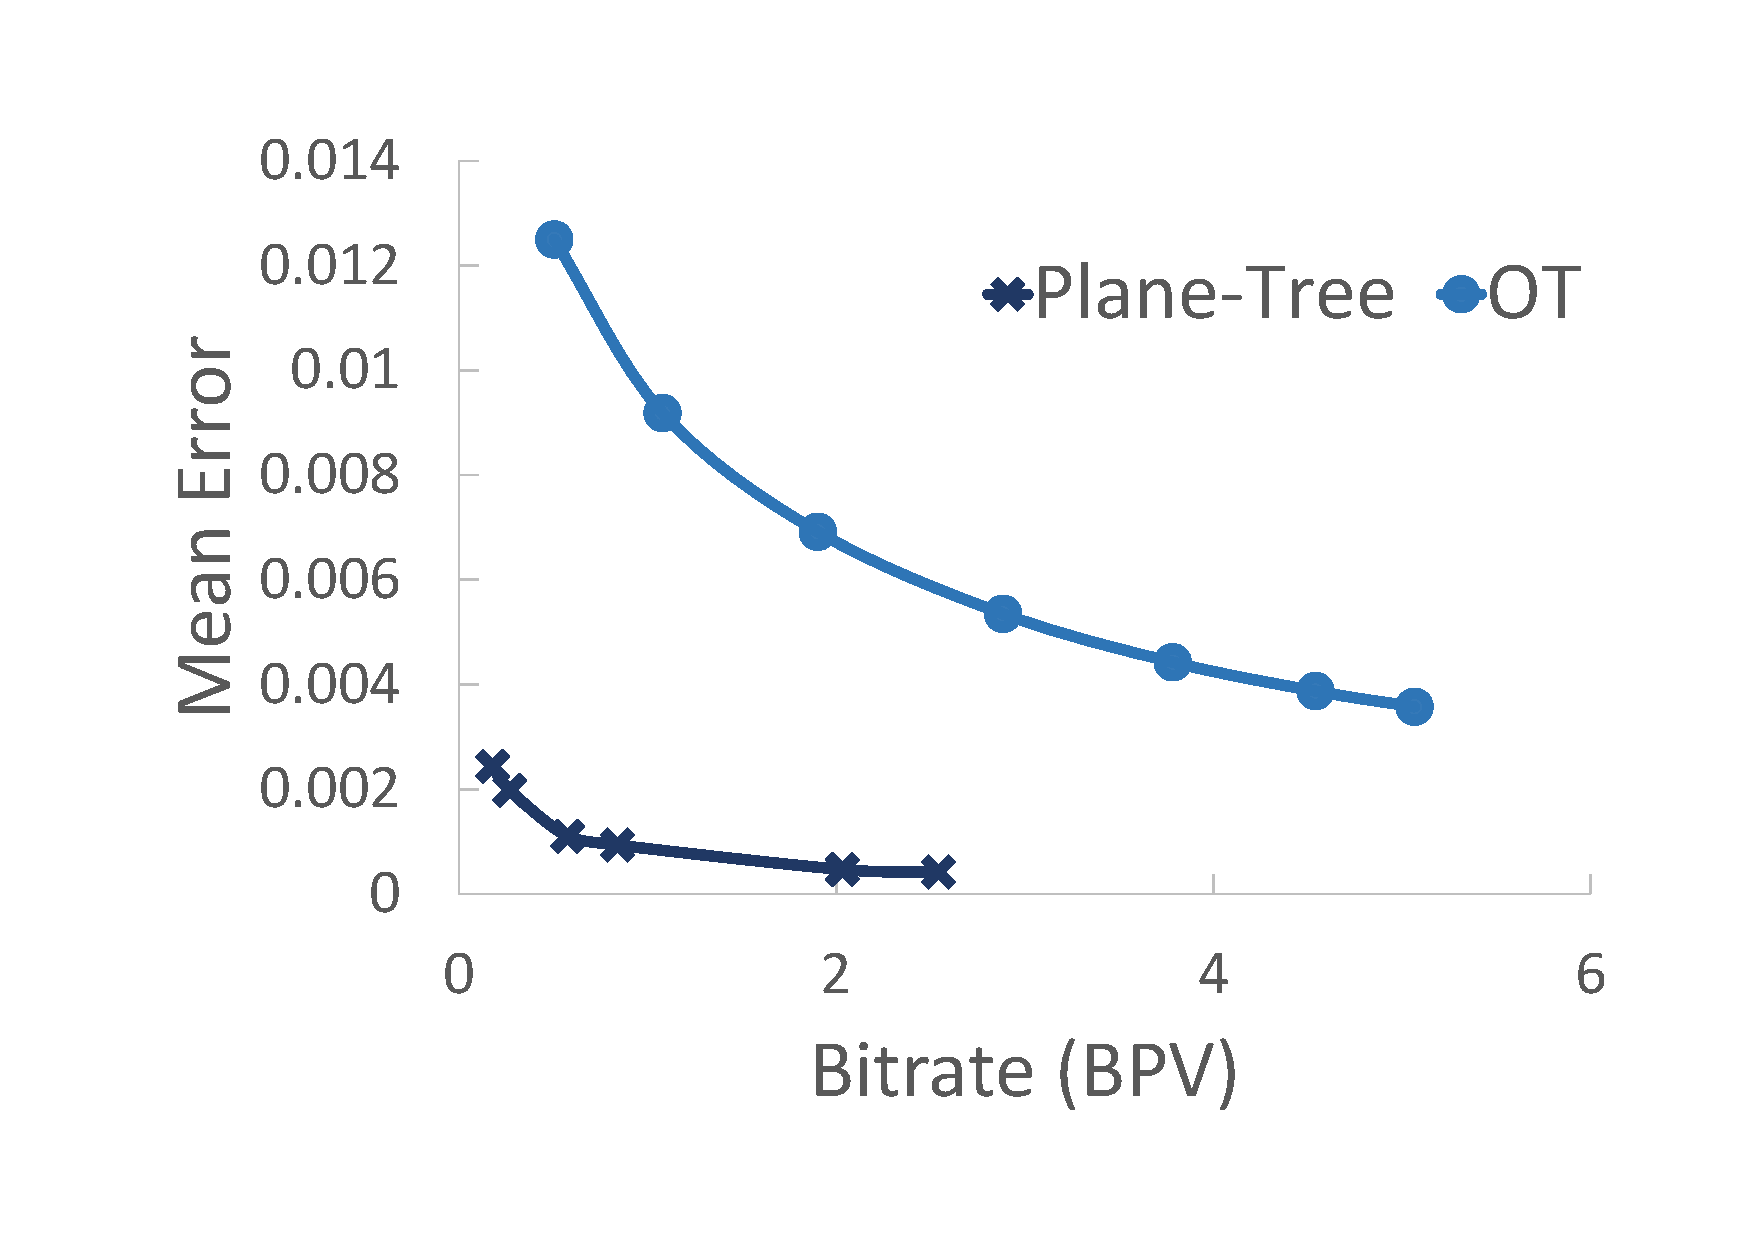
\includegraphics[width=2.5in]{images/results/compression/OTbunny}
                \caption{Bunny Model}
                \label{fig:OG_BUNNY}
        \end{subfigure}
        
        \begin{subfigure}[b]{2.8in}
                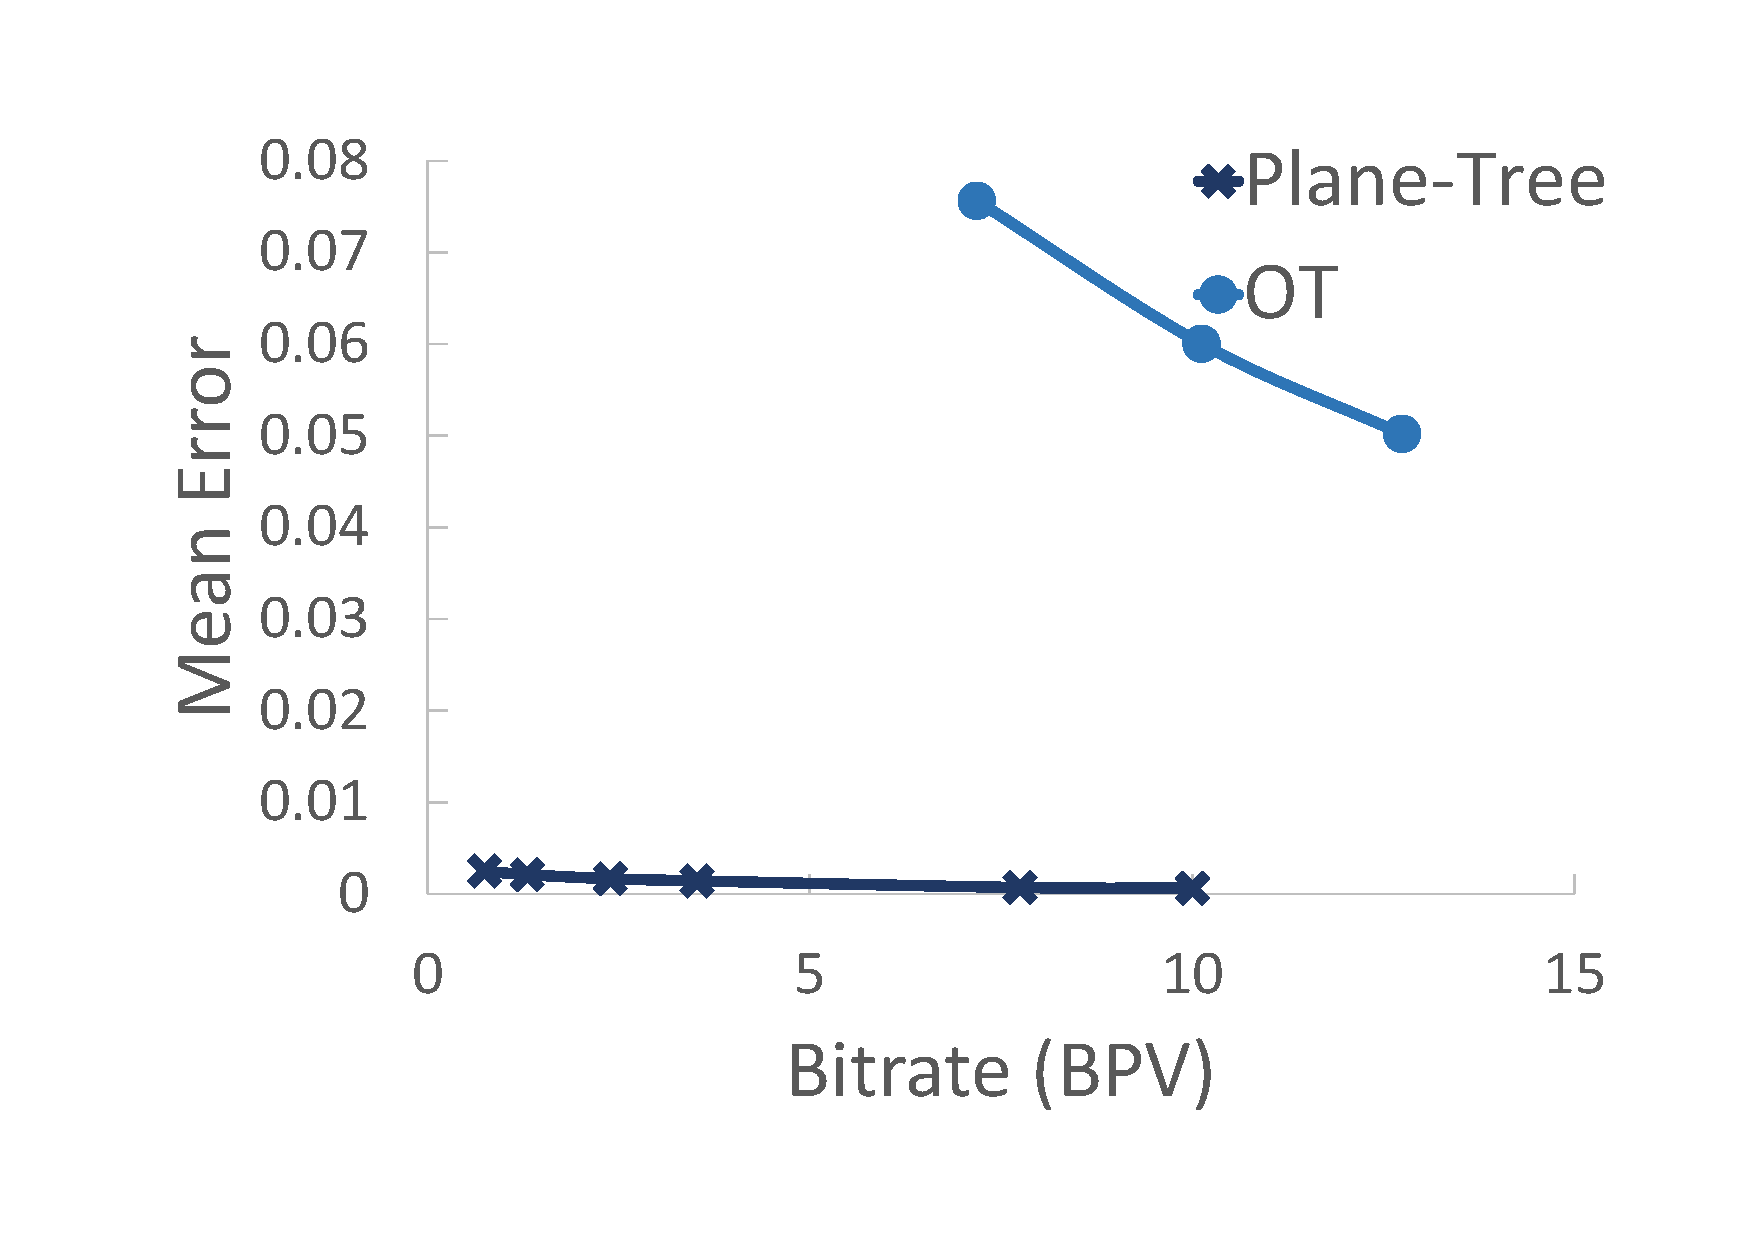
\includegraphics[width=2.5in]{images/results/compression/OTFandisk}
                \caption{Fandisk Model}
                \label{fig:OG_FANDISK}
        \end{subfigure}
        
        \begin{subfigure}[b]{2.8in}
                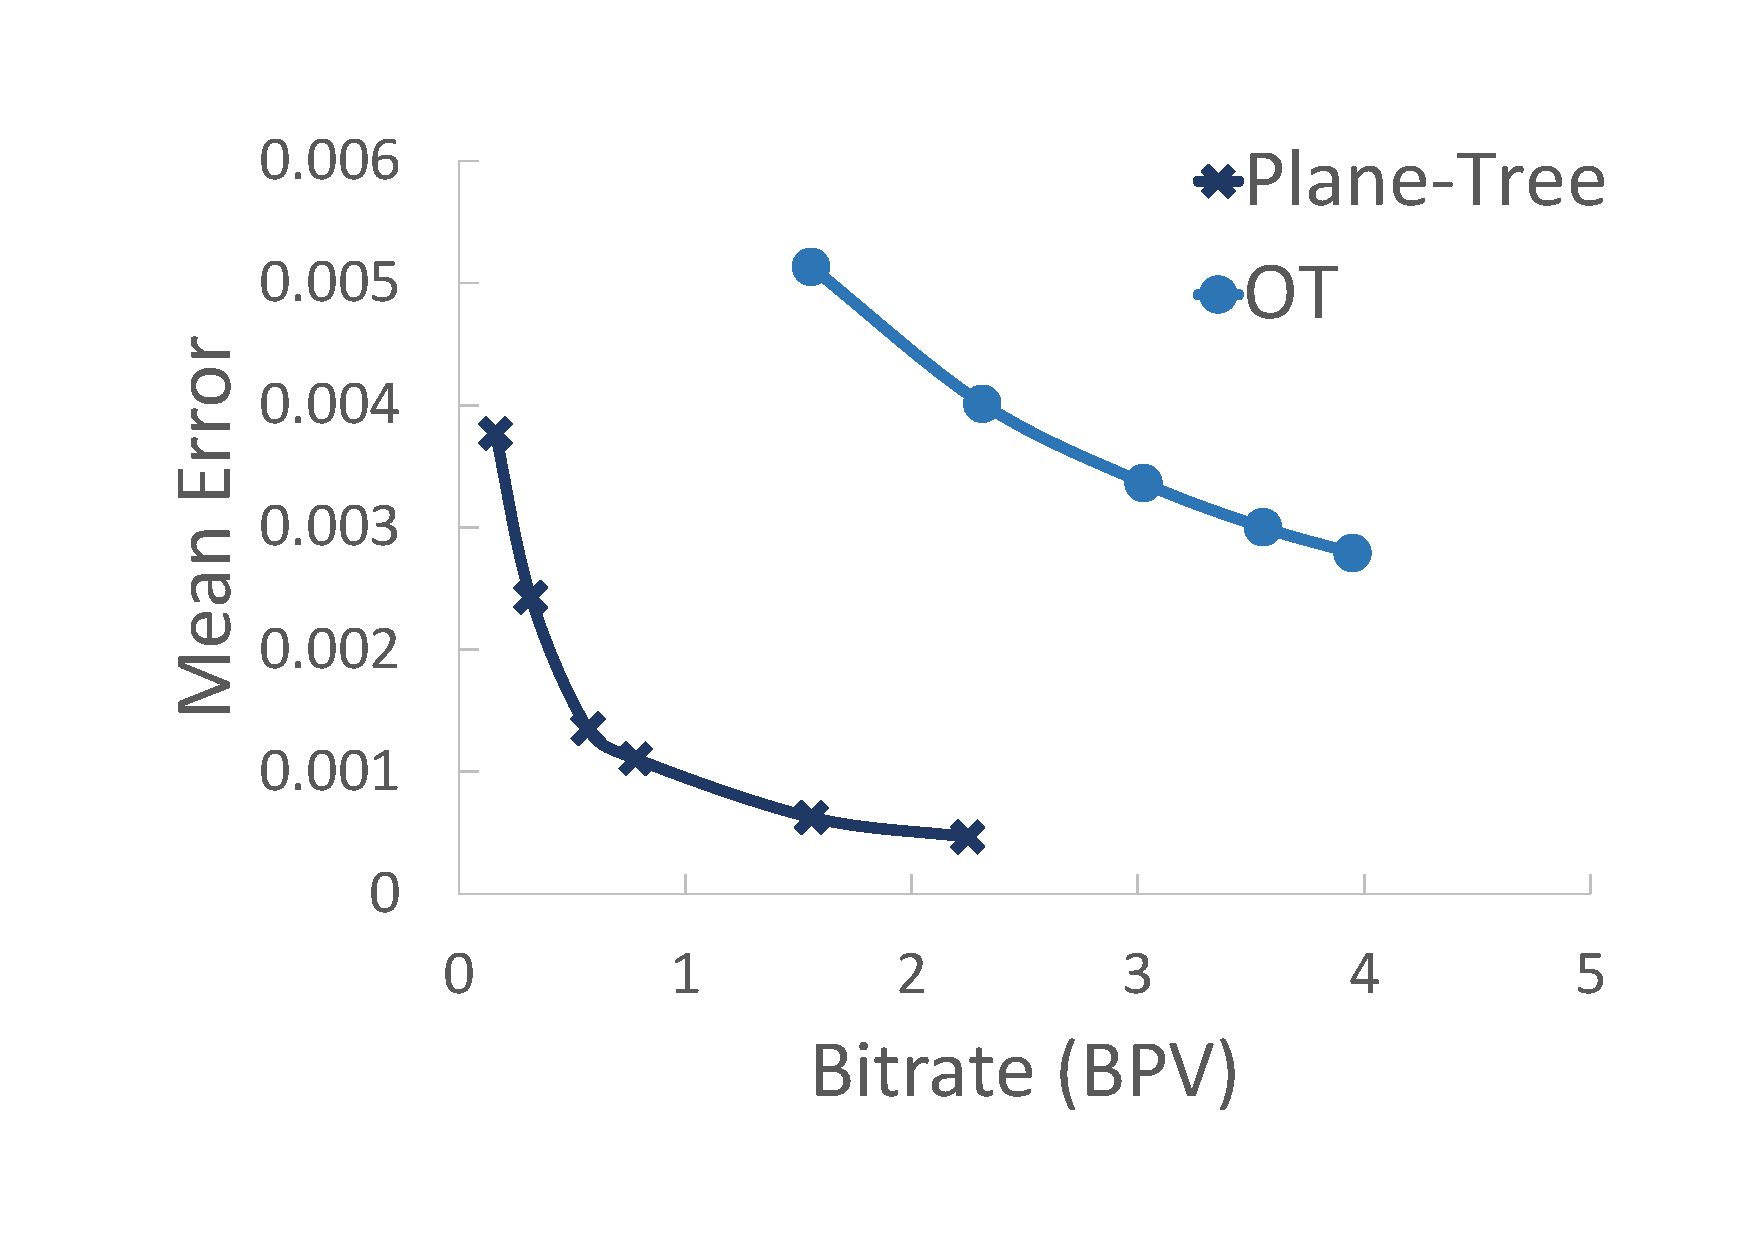
\includegraphics[width=2.5in]{images/results/compression/OTHorse}
                \caption{Horse Model}
                \label{fig:OG_HORSE}
        \end{subfigure}%

       \caption{Rate-distortion graphs comparing the Plane-Tree with the Octree.}
       \label{fig:OTEXPS}
\end{figure}

\subsection{Octree Comparisons}

Figure \ref{fig:OTEXPS} shows rate-distortion graphs comparing the Plane-Tree with the Octree compression method. In these rate-distortion graphs we use the mean error between the decoded and input model as the distortion metric. Results show that for the Bunny and Fandisk experiments (figures \ref{fig:OG_BUNNY} and \ref{fig:OG_FANDISK}) the Plane-Tree has better quality for a given bitrate compared to the Octree. It is also evident that the Octree is unable to reach the level of quality the Plane-Tree reaches. \\

In the Horse model graph in figure \ref{fig:OG_HORSE} there is some overlap in distortion levels. This shows, for a given level of quality the Octree requires around 8 times more storage space compared with the Plane-Tree. \\


\subsection{State of the Art Comparisons}

\begin{figure}[t!] 
        \centering
        \begin{subfigure}[b]{1.8in}
                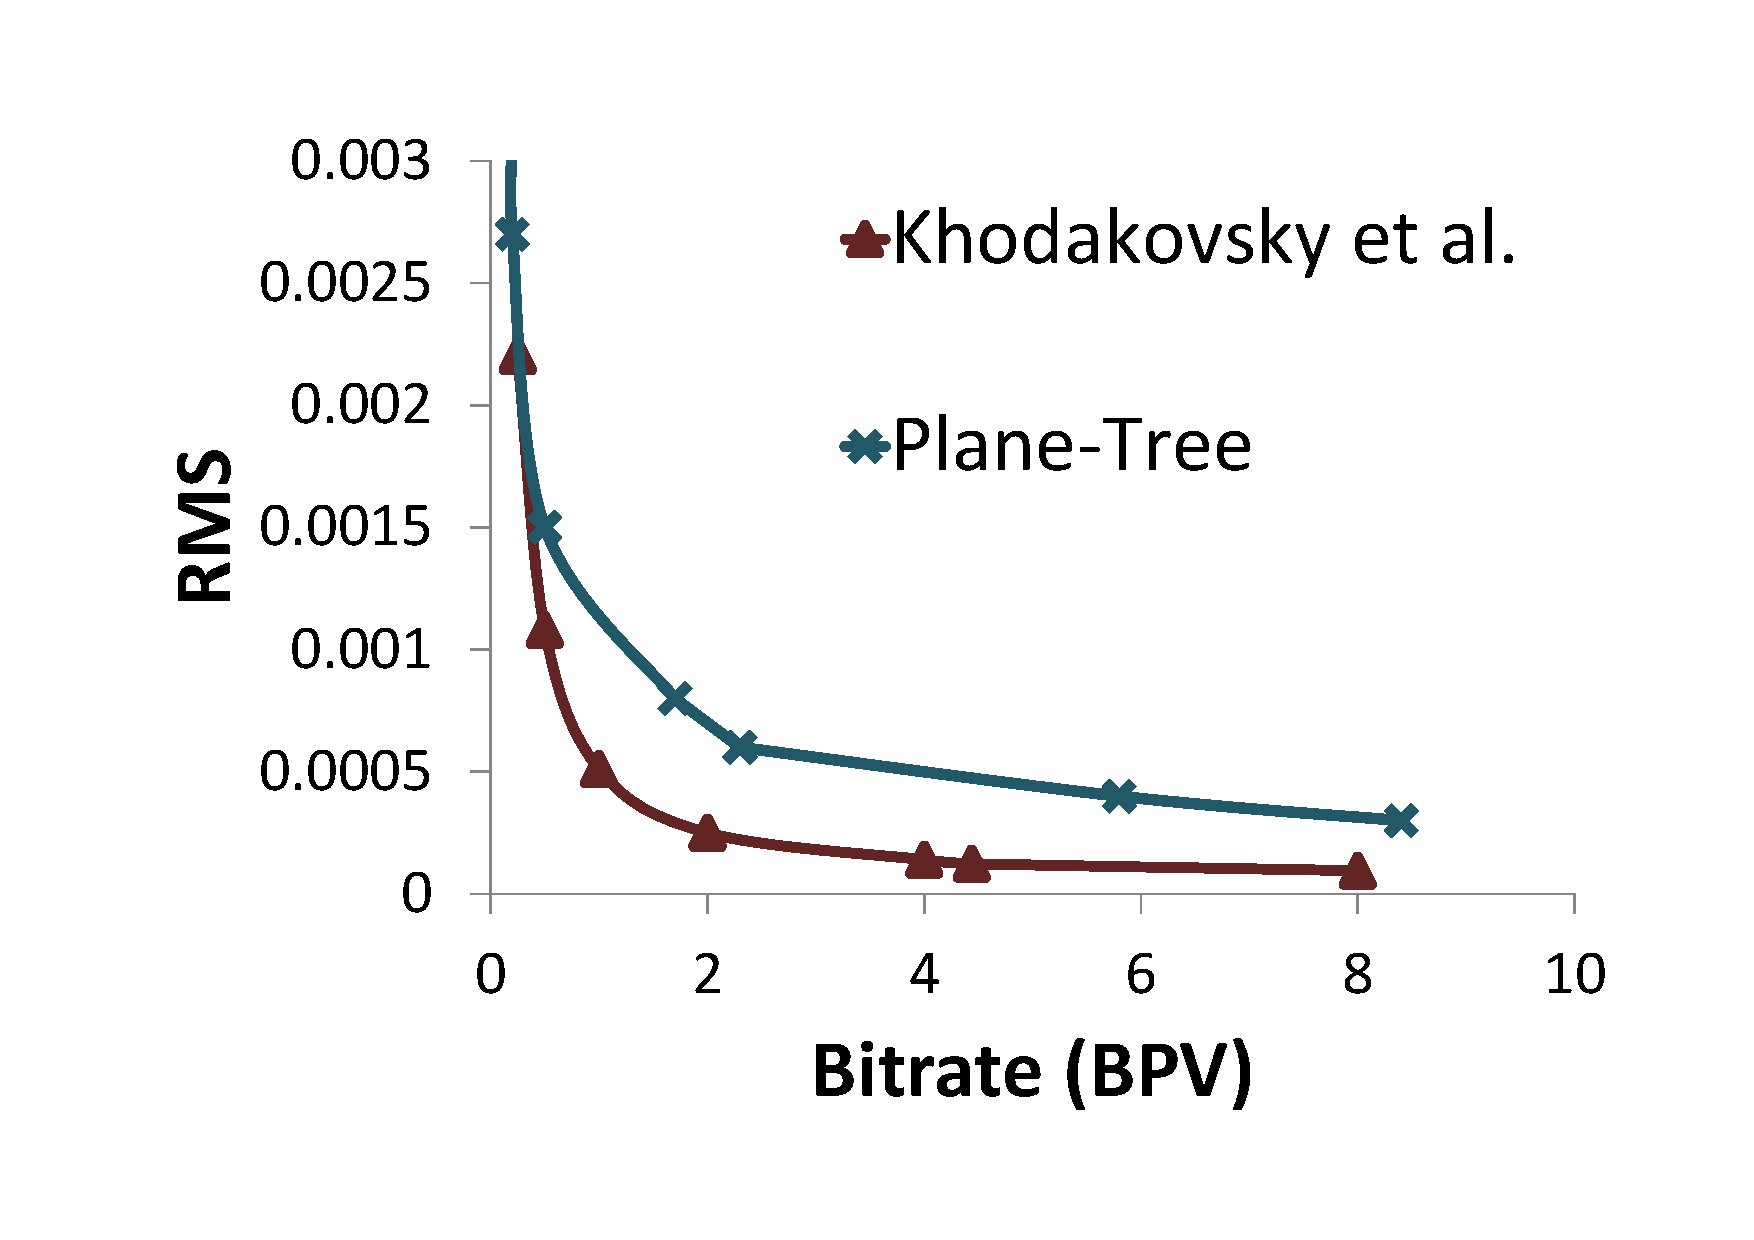
\includegraphics[width=1.8in]{images/results/compression/bunnysota}
                \caption{Bunny Model}
                \label{fig:SA_BUNNY}
        \end{subfigure}%
        \begin{subfigure}[b]{1.8in}
                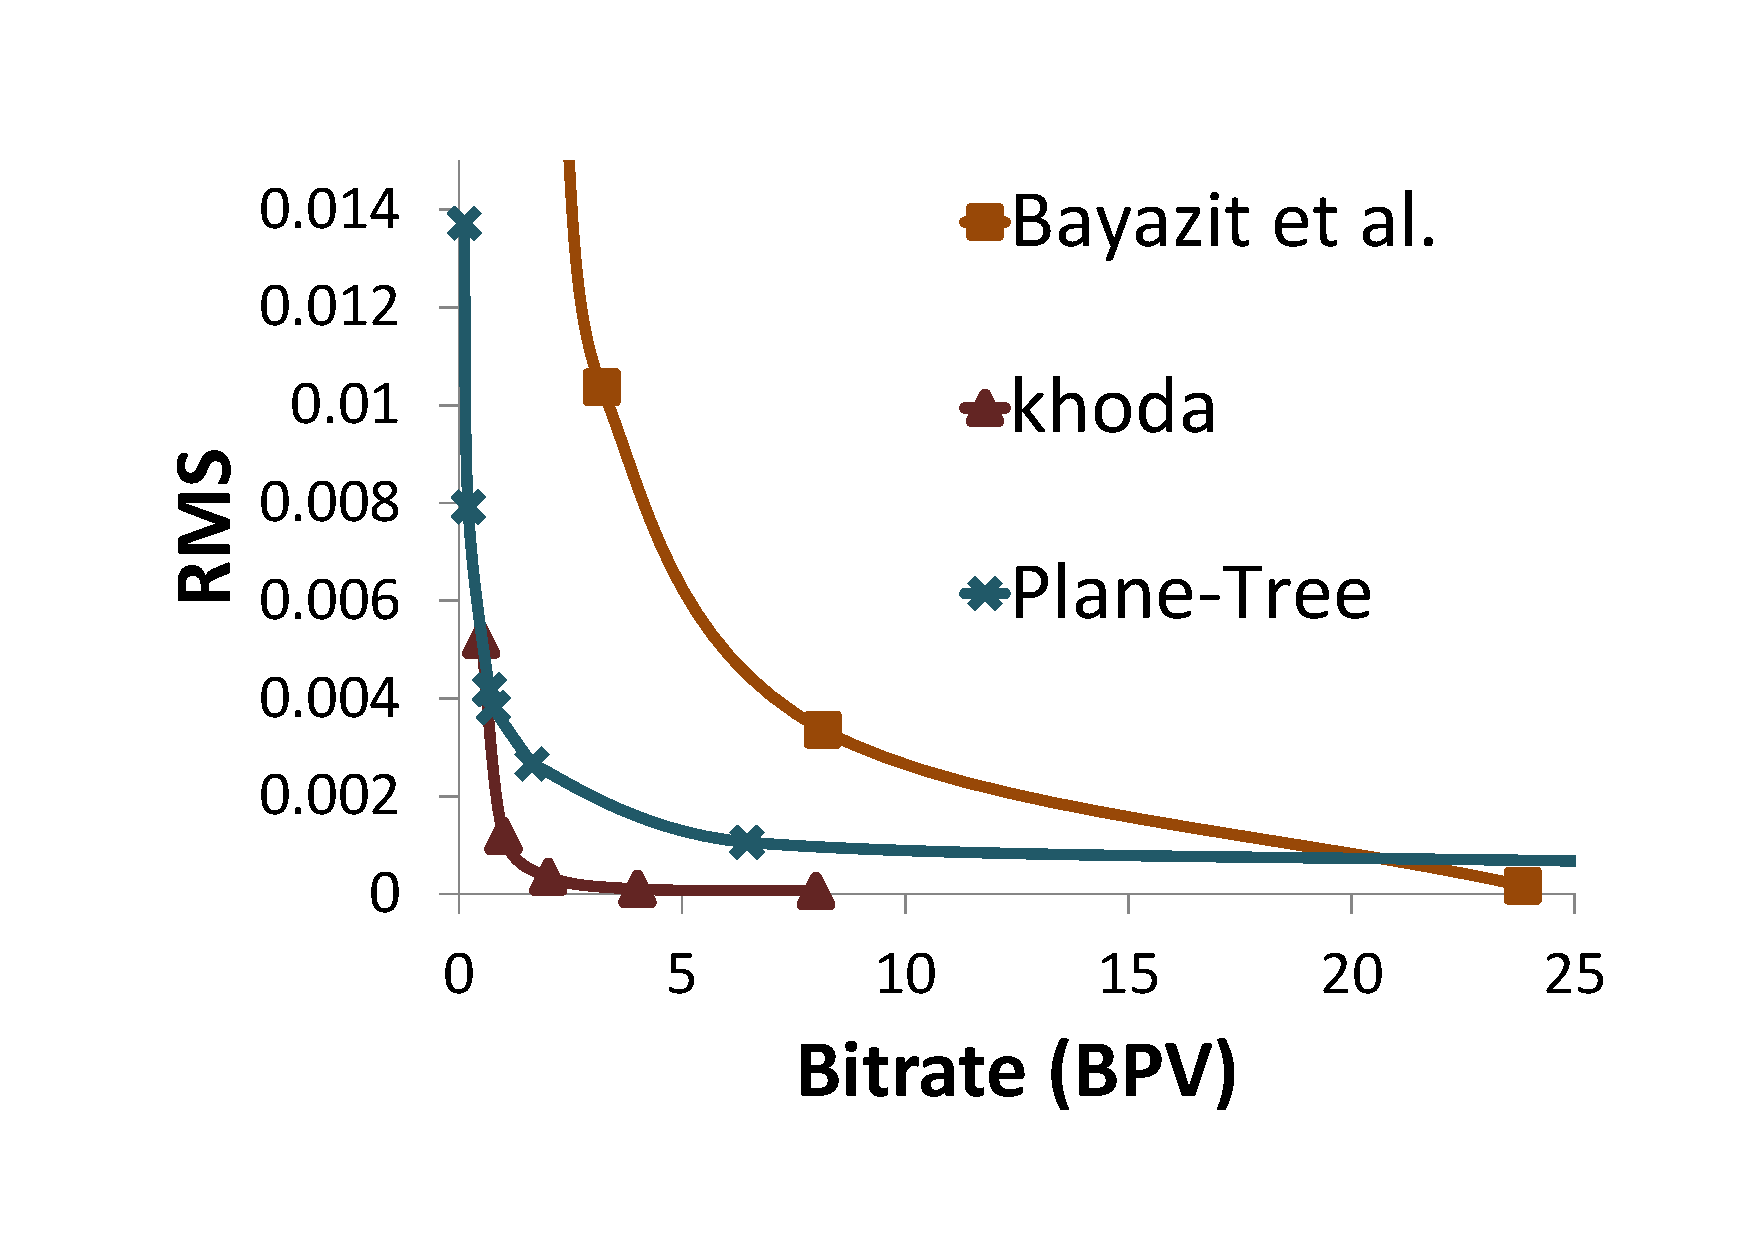
\includegraphics[width=1.8in]{images/results/compression/fandisksota}
                \caption{Fandisk Model}
                \label{fig:SA_FANDISK}
        \end{subfigure}
        
        \begin{subfigure}[b]{1.8in}
                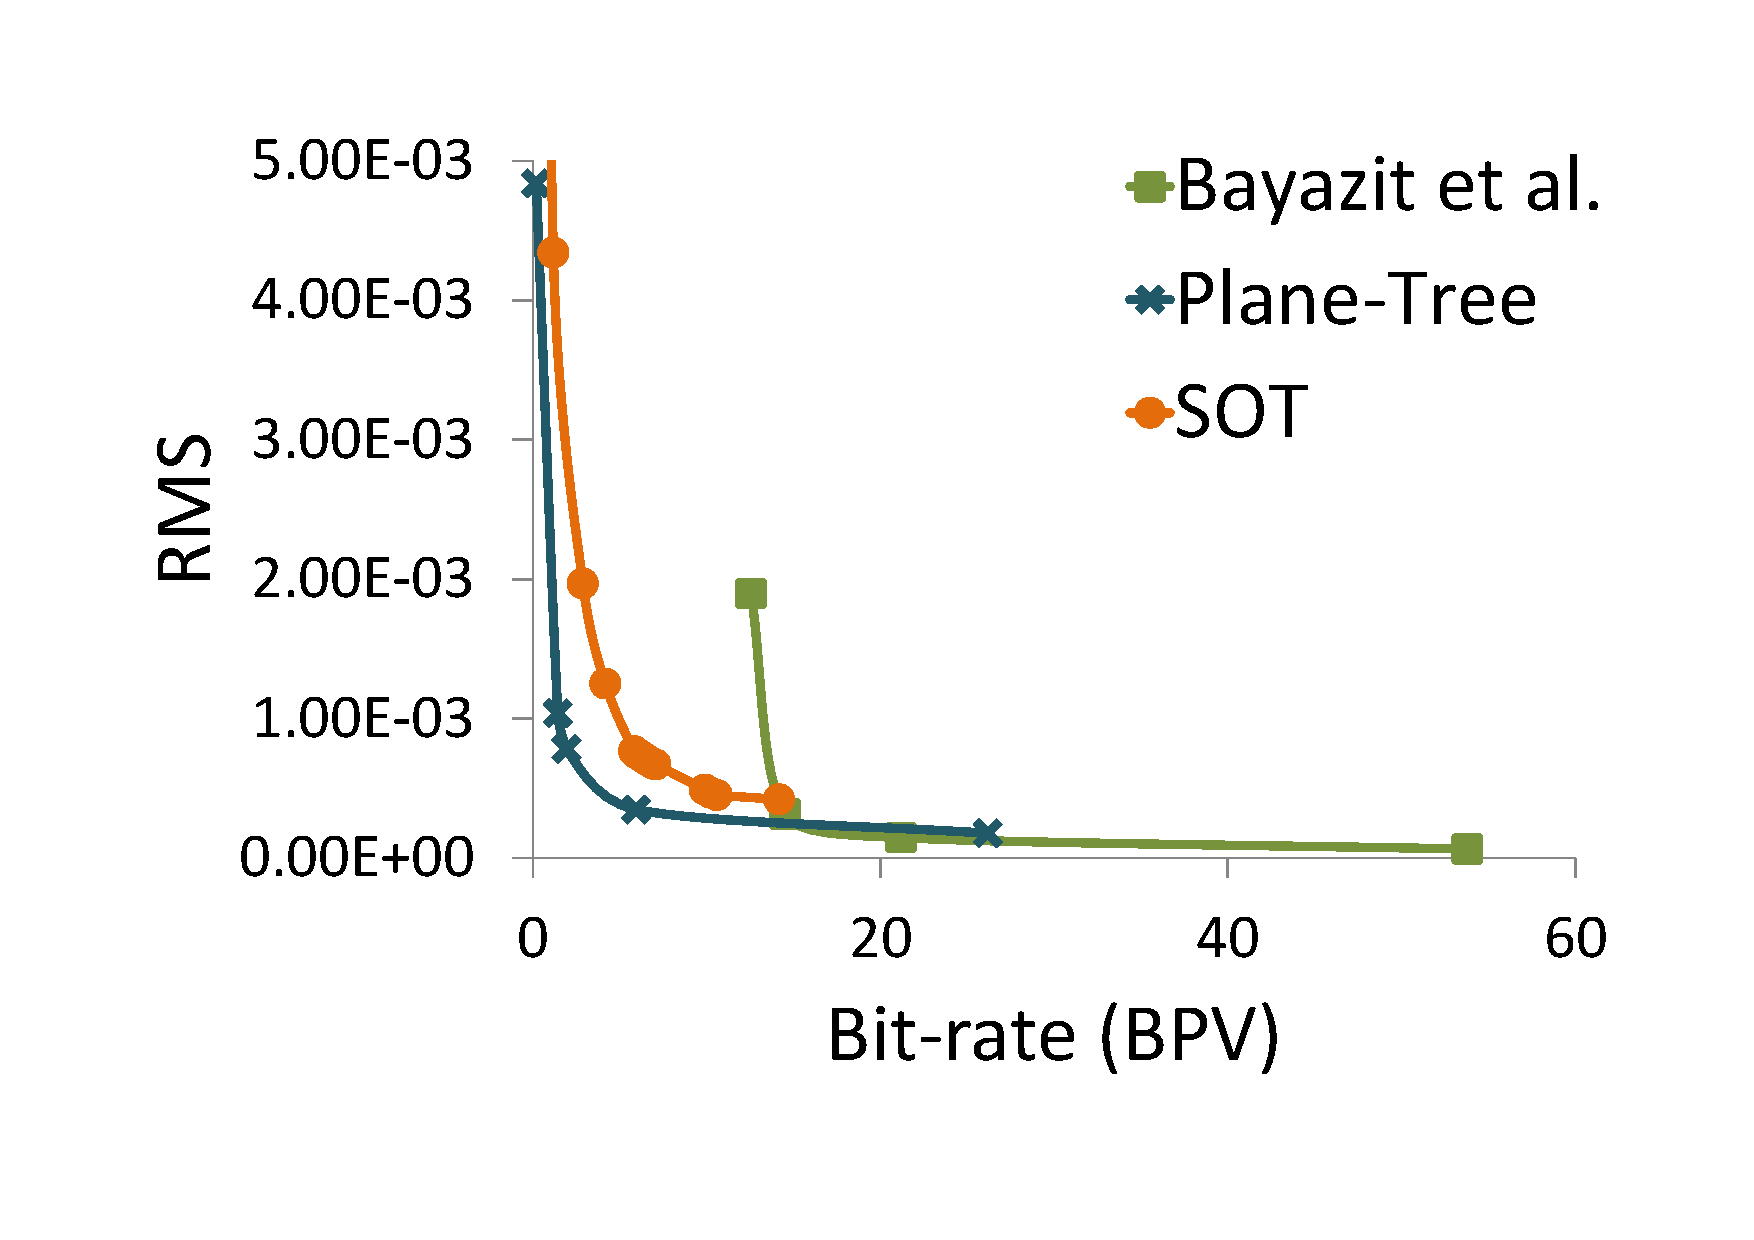
\includegraphics[width=1.8in]{images/results/compression/horsesota}
                \caption{Horse Model}
                \label{fig:SA_HORSE}
        \end{subfigure}%
        \begin{subfigure}[b]{1.8in}
                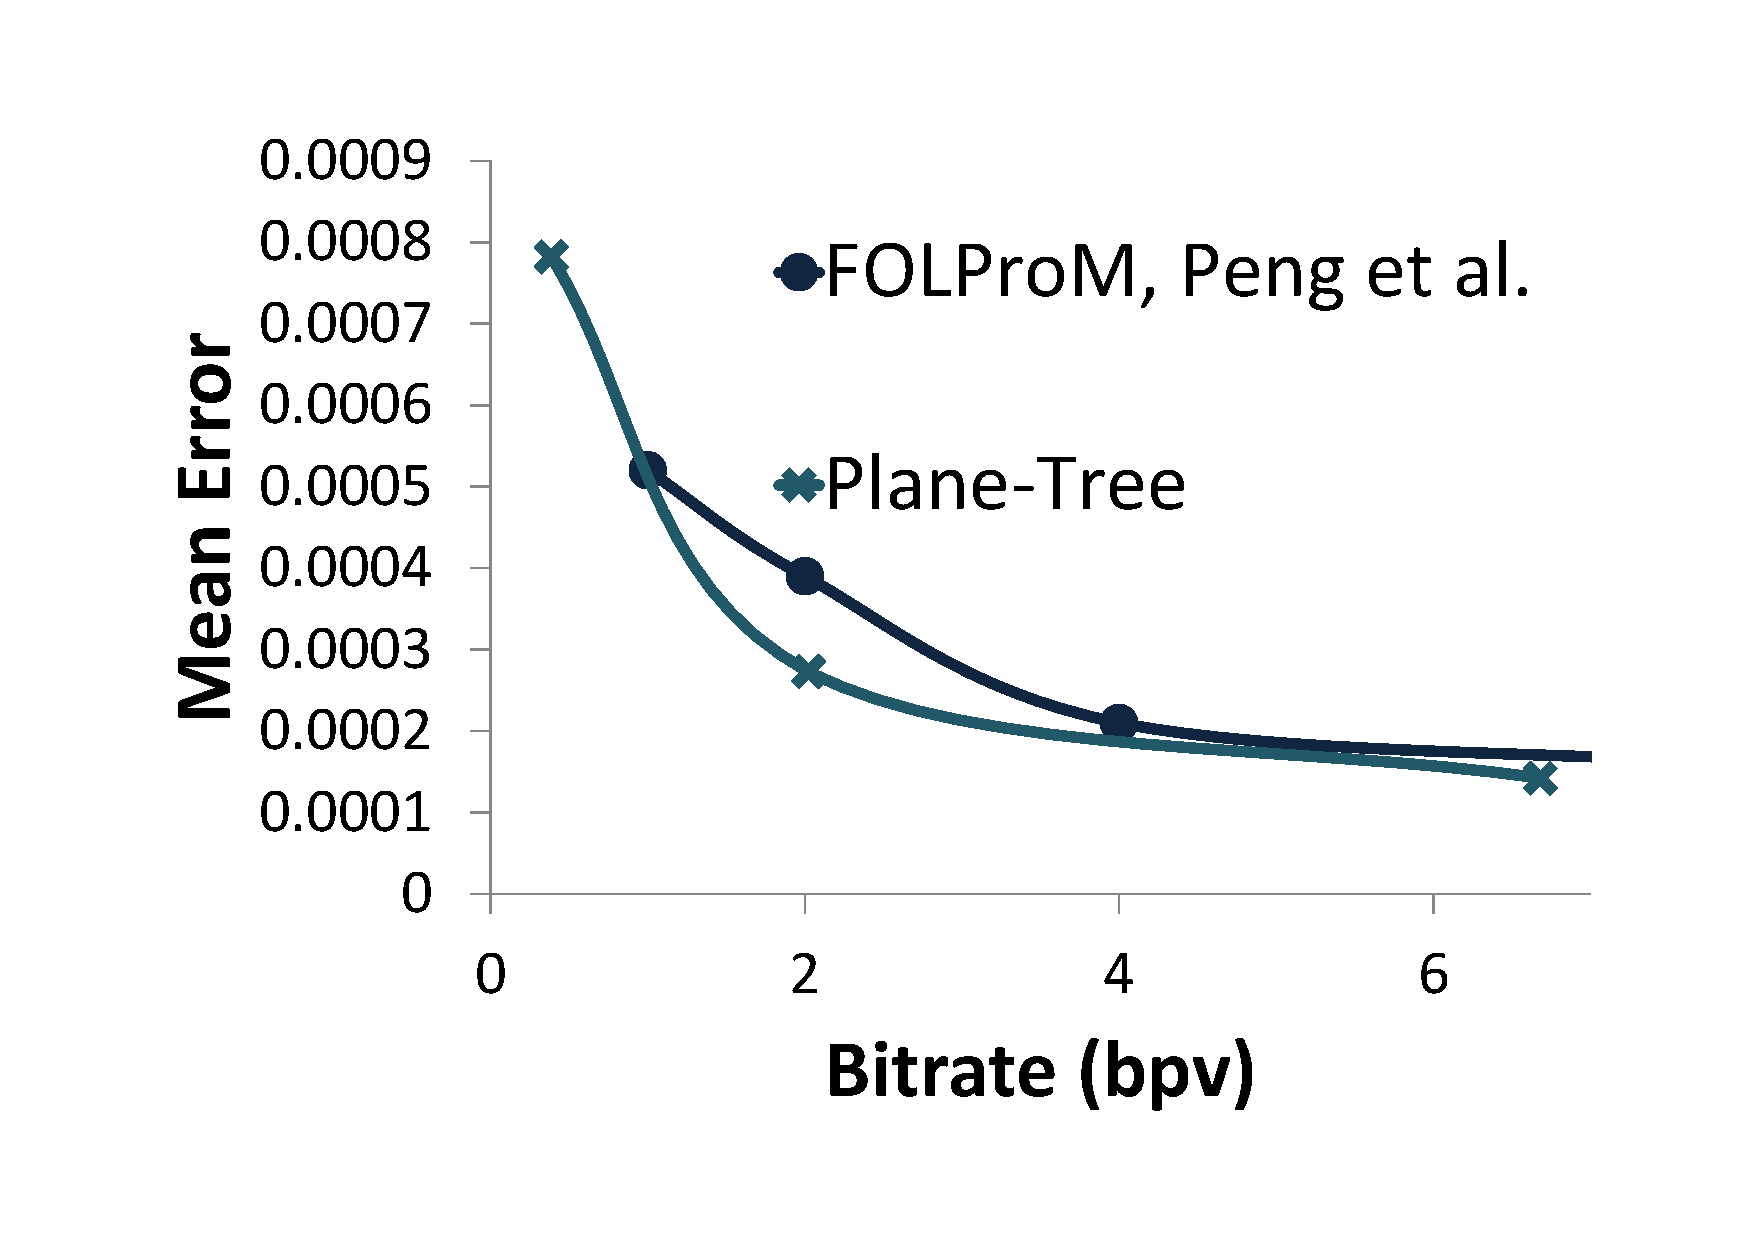
\includegraphics[width=1.8in]{images/results/compression/rabbitsota}
                \caption{Rabbit Model}
                \label{fig:SA_RABBIT}
        \end{subfigure}
       \caption{Rate-Distortion graphs comparing the Plane-Tree to different state of the art codecs.}
       \label{fig:SOTAEXPS}
\end{figure}

In figures \ref{fig:SA_BUNNY}, \ref{fig:SA_FANDISK} and \ref{fig:SA_HORSE} we compare the Plane-Tree with the state of the art transform methods by Bayazit et al \cite{Bayazit103DMesh} and Khodakovsky et al \cite{Khodakovsky00Progressive}. Figure \ref{fig:SA_BUNNY} shows the Plane-Tree has similar distortion compared with the method by Khodakovsky at low-bitrates, whilst being competitive with it up to much higher bitrates. \\

Figure \ref{fig:SA_FANDISK} shows similar results compared with Khodakovsky's method, it also shows the Plane-Tree outperforms the spectral compression method by Bayazit et al at both low and mid level bitrates. Figure \ref{fig:SA_HORSE} shows how the much simpler Plane-Tree method outperforms the transform based method of Bayazit et al. Whilst our method remains competitive at higher bitrates, it outperforms the method by Bayazit at lower bitrates. \\

Finally the Plane-Tree is compared with the state of the art low-bitrate compression system FOLProM \cite{Peng10Feature} using the mean error metric. It can be seen that at low-bitrates (below 2 bits per vertex), the Plane-Tree method outperforms this state of the art low-bitrate compression system. \\

\subsection{Qualitative Results}



\begin{figure*}[t!] 
        \centering
 		\begin{subfigure}[b]{1.9in}
                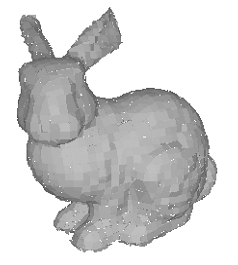
\includegraphics[width=1.6in]{images/results/compression/bunnyb}
                \caption{2.03 bpv\\8827 bytes}
                \label{fig:FIG_BUNNYB}
        \end{subfigure}%
        \begin{subfigure}[b]{1.9in}
                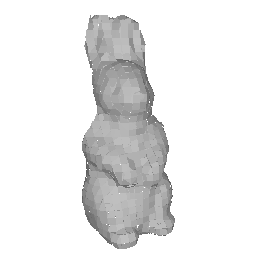
\includegraphics[width=1.6in]{images/results/compression/rabbitb}
                \caption{0.47\\3898 bytes}
                \label{fig:FIG_RABBITB}
        \end{subfigure}%
        \begin{subfigure}[b]{1.9in}
                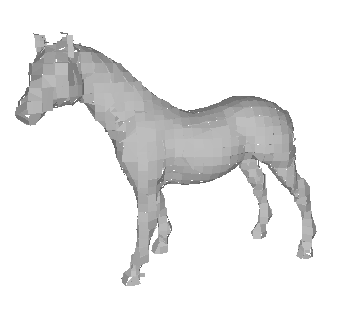
\includegraphics[width=1.6in]{images/results/compression/horseb}
                \caption{1.55 bpv\\3842 bytes}
                \label{fig:FIG_HORSEB}
        \end{subfigure}

        \begin{subfigure}[b]{1.9in}
                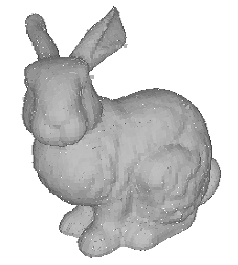
\includegraphics[width=1.6in]{images/results/compression/bunnyd}
                \caption{7.74 bpv\\33701 bytes}
                \label{fig:FIG_BUNNYD}
        \end{subfigure}%
        \begin{subfigure}[b]{1.9in}
                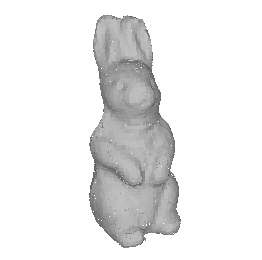
\includegraphics[width=1.6in]{images/results/compression/rabbitd}
                \caption{1.97\\16492 bytes}
                \label{fig:FIG_RABBITD}
        \end{subfigure}%
        \begin{subfigure}[b]{1.9in}
                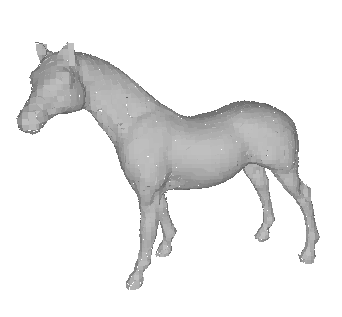
\includegraphics[width=1.6in]{images/results/compression/horsed}
                \caption{5.95 bpv\\14758 bytes}
                \label{fig:FIG_HORSED}
        \end{subfigure}
        
        \begin{subfigure}[b]{1.9in}
                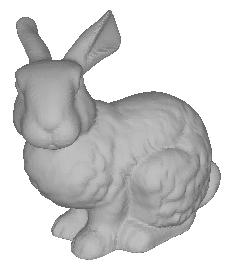
\includegraphics[width=1.6in]{images/results/compression/bunnyorig}
                \caption{original: 518.78 bpv\\2,258,902 bytes}
                \label{fig:FIG_BUNNYO}
        \end{subfigure}%
        \begin{subfigure}[b]{1.9in}
                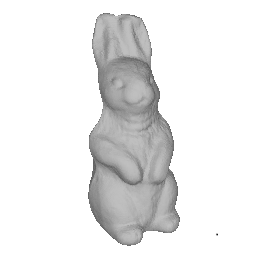
\includegraphics[width=1.6in]{images/results/compression/rabbitorig}
                \caption{original: 530.14\\4,442,413 bytes}
                \label{fig:FIG_RABBITO}
        \end{subfigure}%
        \begin{subfigure}[b]{1.9in}
                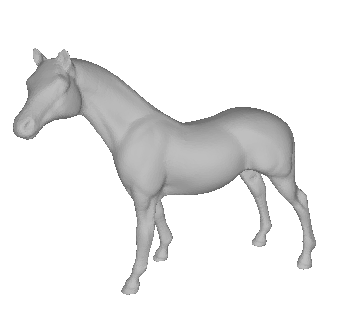
\includegraphics[width=1.6in]{images/results/compression/horseorig}
                \caption{original: 519.92 bpv\\1,290,120 bytes}
                \label{fig:FIG_HORSEO}
        \end{subfigure}
       
       \caption{Models coded with our coder at thresholds of 8.0 and 1.0 with a maximum tree depth of 6 along with the original models.}
       \label{fig:FIGS}
\end{figure*}

In figure \ref{fig:FIGS} we present qualitative results for the Plane-Tree. The third row shows the bunny, rabbit and horse models along with the number of bytes and bpv required to store them uncompressed. The first row shows each model compressed by the Plane-Tree with a threshold of 8.0. Despite these being crude approximations of the originals, the models are still distinguishable with around 1000 $\times$ less storage space required. \\

In the second row, each model was compressed with the Plane-Tree at a threshold of 1.0. In these experiments there is little detail missing compared with the physical model. When looking at the bunny's legs, the same ripples are present. In the rabbit model, the outlines inside the ears and on the eyes are still present. On the horse model, the creases on the body and shoulder of the horse are still present. Here, the bunny is compressed to around 70 $\times$ less storage space, the rabbit at around 265 $\times$ less and the horse around 90 $\times$ less storage space. \\




here we compare the volumetric plane-tree to the ot, the other methods are designed for mesh compression and since the ot is one of the most common representations used for 3d reconstruction we compare with it. we also have an implementation of ilqt extended to 3d called the ilot (interpolating leaf oct-tree) we compare with. Results show that for low bit-rates the ilot outperforms the ot. However as higher quality is required, OT outperforms this. The plane-tree which was the original envisionment of iqlt for 3D data is shown to improve upon the OT and ILOT at both low and high bit-rates. \\

\begin{figure*}[t]
\centering
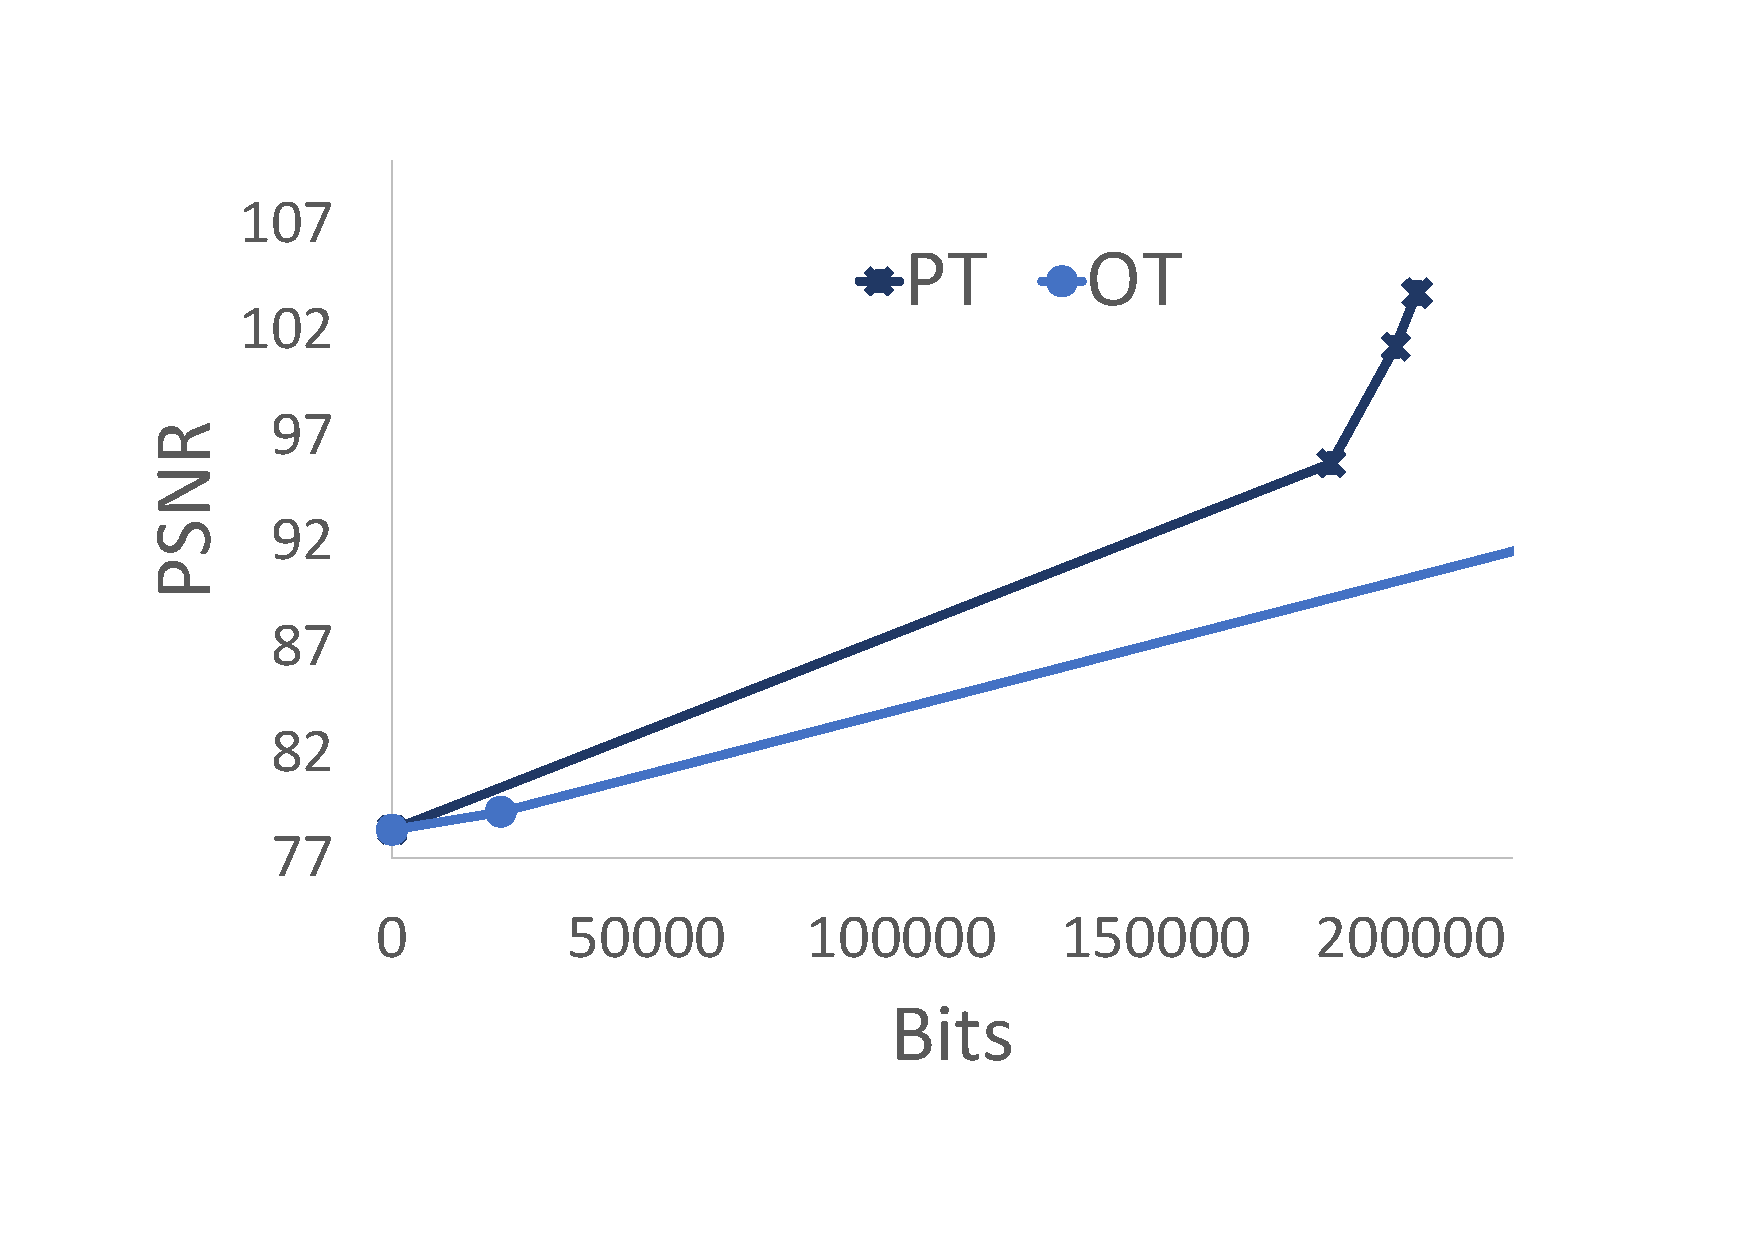
\includegraphics[width=6.0in]{images/results/compression/psnr1}
\caption{PSNR vs Bitrate comparing the ILOT, OT and PT compression methods.}
\label{fig:PSNR1}
\end{figure*}

By reducing the size of 3D reconstructions processing speed and storage will be advanced. This is advantageous in 3D reconstruction as we may want to transmit reconstructions over a network (from a robot to a base station for example). By using an advanced compression scheme we can transmit this data faster. 


\section{Conclusion}
